%Template para TCC CIC UFRGS
%Author: Lucas Schnorr (Adaptado para overleaf por Rubens dos Santos)

% exemplo genérico de uso da classe iiufrgs.cls
% $Id: iiufrgs.tex,v 1.1.1.1 2005/01/18 23:54:42 avila Exp $
% 
% This is an example file and is hereby explicitly put in the
% public domain.
% 
\documentclass[ecp,tc,english]{iiufrgs}
% Para usar o modelo, deve-se informar o programa e o tipo de documento.
% Programas :
% * cic       -- Graduação em Ciência da Computação
% * ecp       -- Graduação em Ciência da Computação
% * ppgc      -- Programa de Pós Graduação em Computação
% * pgmigro   -- Programa de Pós Graduação em Microeletrônica
% 
% Tipos de Documento:
% * tc                -- Trabalhos de Conclusão (apenas cic e ecp)
% * diss ou mestrado  -- Dissertações de Mestrado (ppgc e pgmicro)
% * tese ou doutorado -- Teses de Doutorado (ppgc e pgmicro)
% * ti                -- Trabalho Individual (ppgc e pgmicro)
% 
% Outras Opções:
% * english    -- para textos em inglês
% * openright  -- Força início de capítulos em páginas ímpares (padrão da
% biblioteca)
% * oneside    -- Desliga frente-e-verso
% * nominatalocal -- Lê os dados da nominata do arquivo nominatalocal.def


% Use unicode
\usepackage[utf8]{inputenc}   % pacote para acentuação
\DeclareUnicodeCharacter{200B}{} % ignora o espaço de largura zero que vem em textos colados

% Necessário para incluir figuras
\usepackage{graphicx}         % pacote para importar figuras

\usepackage{times}            % pacote para usar fonte Adobe Times
% \usepackage{palatino}
% \usepackage{mathptmx}       % p/ usar fonte Adobe Times nas fórmulas

\usepackage{amsmath,amssymb}  % pacotes para ambientes e símbolos matemáticos

\usepackage[alf,abnt-emphasize=bf]{abntex2cite}	% pacote para usar citações abnt
\newcommand{\citesp}[1]{\citeauthor{#1}, \citeyear{#1}} % citação sem parênteses (fontes das tabelas)

% --- PACOTES ADICIONADOS PARA O DESENHO DAS MATRIZES ---
\usepackage{placeins}         % \FloatBarrier: figuras de um grupo não passam para o próximo
% 2026-11-11: folgas maiores para figuras grandes ficarem na mesma página do texto, em vez de
%   irem sozinhas para uma página (padrão: topfraction 0,7, textfraction 0,2, floatpagefraction 0,5)
\renewcommand{\topfraction}{0.9}
\renewcommand{\bottomfraction}{0.8}
\renewcommand{\textfraction}{0.07}
\renewcommand{\floatpagefraction}{0.8}
\setcounter{topnumber}{3}
\setcounter{totalnumber}{4}
\usepackage{booktabs}         % tabelas com \toprule, \midrule e \bottomrule
\usepackage{multirow}         % células mescladas nas tabelas
\usepackage[normalem]{ulem}     % texto riscado (\sout) nas revisões do capítulo
\definecolor{RED}{rgb}{1,0,0} % a classe põe títulos de capítulo em maiúsculas: \textcolor{red} vira \textcolor{RED}
% Larguras do sumario fixas. O tocstyle (tocindentauto) recalcula essas larguras
% a cada passada e so estabiliza na 5a; fixando, o Overleaf converge em 3.
% Se aparecer figura/tabela/secao com numeracao mais larga (ex.: Figure 4.10) e o
% sumario ou as listas ficarem desalinhados, apague este bloco, compile ate
% estabilizar e recopie os valores de \tocstyle@set@width do 0main.aux.
\makeatletter
\AtBeginDocument{%
  \gdef\tocstyle@maxunumwidth@lof@{27.0pt}%
  \gdef\tocstyle@maxnumwidth@lof@1{27.0pt}%
  \gdef\tocstyle@maxskipwidth@lof@1{18.0pt}%
  \gdef\tocstyle@maxunumwidth@lot@{23.66396pt}%
  \gdef\tocstyle@maxnumwidth@lot@1{23.66396pt}%
  \gdef\tocstyle@maxskipwidth@lot@1{18.0pt}%
  \gdef\tocstyle@maxunumwidth@toc@{39.0pt}%
  \gdef\tocstyle@maxskipwidth@toc@0{0.0pt}%
  \gdef\tocstyle@maxnumwidth@toc@1{23.66396pt}%
  \gdef\tocstyle@maxskipwidth@toc@1{18.0pt}%
  \gdef\tocstyle@maxnumwidth@toc@2{30.0pt}%
  \gdef\tocstyle@maxskipwidth@toc@2{41.66396pt}%
  \gdef\tocstyle@maxnumwidth@toc@3{39.0pt}%
  \gdef\tocstyle@maxskipwidth@toc@3{71.66396pt}%
  \renewcommand*{\tocstyle@post@starttoc}[1]{\endgroup}% nao regrava as larguras no .aux
}
\makeatother


% 
% Informações gerais
% 
\title{Hardware Accelerator for Matrix Inversion in Decentralized Massive MIMO LMMSE Equalization Under Colored Noise}

\author{de Vargas}{Juliana Rodrigues}
% alguns documentos podem ter varios autores:
% \author{Flaumann}{Frida Gutenberg}
% \author{Flaumann}{Klaus Gutenberg}

% orientador e co-orientador são opcionais (não diga isso pra eles :))
\advisor[Prof.~Dr.]{Lamport}{Leslie}
\coadvisor[Prof.~Dr.]{Knuth}{Donald Ervin}

% a data deve ser a da defesa; se nao especificada, são gerados
% mes e ano correntes
% \date{maio}{2001}

% o local de realização do trabalho pode ser especificado (ex. para TCs)
% com o comando \location:
% \location{Itaquaquecetuba}{SP}

% itens individuais da nominata podem ser redefinidos com os comandos
% abaixo:
% \renewcommand{\nominataReit}{Prof\textsuperscript{a}.~Wrana Maria Panizzi}
% \renewcommand{\nominataReitname}{Reitora}
% \renewcommand{\nominataPRE}{Prof.~Jos{\'e} Carlos Ferraz Hennemann}
% \renewcommand{\nominataPREname}{Pr{\'o}-Reitor de Ensino}
% \renewcommand{\nominataPRAPG}{Prof\textsuperscript{a}.~Joc{\'e}lia Grazia}
% \renewcommand{\nominataPRAPGname}{Pr{\'o}-Reitora Adjunta de P{\'o}s-Gradua{\c{c}}{\~a}o}
% \renewcommand{\nominataDir}{Prof.~Philippe Olivier Alexandre Navaux}
% \renewcommand{\nominataDirname}{Diretor do Instituto de Inform{\'a}tica}
% \renewcommand{\nominataCoord}{Prof.~Carlos Alberto Heuser}
% \renewcommand{\nominataCoordname}{Coordenador do PPGC}
% \renewcommand{\nominataBibchefe}{Beatriz Regina Bastos Haro}
% \renewcommand{\nominataBibchefename}{Bibliotec{\'a}ria-chefe do Instituto de Inform{\'a}tica}
% \renewcommand{\nominataChefeINA}{Prof.~Jos{\'e} Valdeni de Lima}
% \renewcommand{\nominataChefeINAname}{Chefe do \deptINA}
% \renewcommand{\nominataChefeINT}{Prof.~Leila Ribeiro}
% \renewcommand{\nominataChefeINTname}{Chefe do \deptINT}

% A seguir são apresentados comandos específicos para alguns
% tipos de documentos.

% Relatório de Pesquisa [rp]:
% \rp{123}             % numero do rp
% \financ{CNPq, CAPES} % orgaos financiadores

% Trabalho Individual [ti]:
% \ti{123}     % numero do TI
% \ti[II]{456} % no caso de ser o segundo TI

% Monografias de Especialização [espec]:
% \espec{Redes e Sistemas Distribuídos}      % nome do curso
% \coord[Profa.~Dra.]{Weber}{Taisy da Silva} % coordenador do curso
% \dept{INA}                                 % departamento relacionado

% 
% palavras-chave
% iniciar todas com letras minúsculas, exceto no caso de abreviaturas
% 
\keyword{formatação eletrônica de documentos}
\keyword{\LaTeX}
\keyword{ABNT}
\keyword{UFRGS}

%\settowidth{\seclen}{1.10~}

% 
% inicio do documento
% 
% deixa o LaTeX esticar um pouco os espaços antes de estourar a margem direita
\setlength{\emergencystretch}{1.5em}
\begin{document}

% folha de rosto
% às vezes é necessário redefinir algum comando logo antes de produzir
% a folha de rosto:
% \renewcommand{\coordname}{Coordenadora do Curso}
\maketitle

% dedicatoria
% \clearpage
% \begin{flushright}
%     \mbox{}\vfill
%     {\sffamily\itshape
%       ``If I have seen farther than others,\\
%       it is because I stood on the shoulders of giants.''\\}
%     --- \textsc{Sir~Isaac Newton}
% \end{flushright}

% agradecimentos
%\chapter*{Agradecimentos}
%Agradeço ao \LaTeX\ por não ter vírus de macro\ldots



% resumo na língua do documento
\begin{abstract}
    Este documento é um exemplo de como formatar documentos para o
    Instituto de Informática da UFRGS usando as classes \LaTeX\
    disponibilizadas pelo UTUG\@. Ao mesmo tempo, pode servir de consulta
    para comandos mais genéricos. \emph{O texto do resumo não deve
      conter mais do que 500 palavras.}
\end{abstract}

% resumo na outra língua
% como parametros devem ser passados o titulo e as palavras-chave
% na outra língua, separadas por vírgulas
\begin{englishabstract}{Using \LaTeX\ to Prepare Documents at II/UFRGS}{Electronic document preparation. \LaTeX. ABNT. UFRGS}
    This document is an example on how to prepare documents at II/UFRGS
    using the \LaTeX\ classes provided by the UTUG\@. At the same time, it
    may serve as a guide for general-purpose commands. \emph{The text in
      the abstract should not contain more than 500~words.}
\end{englishabstract}

% lista de figuras
\listoffigures

% lista de tabelas
\listoftables

% lista de abreviaturas e siglas
% o parametro deve ser a abreviatura mais longa
\begin{listofabbrv}{QuaDRiGa}
    \item[3GPP] 3rd Generation Partnership Project
    \item[5G] Quinta geração de redes móveis
    \item[AoA] Angle of Arrival
    \item[AoD] Angle of Departure
    \item[AWGN] Additive White Gaussian Noise
    \item[BCD] Block Coordinate Descent
    \item[BS] Base Station
    \item[DM-RS] Demodulation Reference Signal
    \item[DU] Distributed Unit
    \item[FR1] Frequency Range 1
    \item[FR2] Frequency Range 2
    \item[HST] High Speed Train
    \item[InF] Indoor Factory
    \item[InH] Indoor Hotspot
    \item[IoTh] \textcolor{red}{Interference over Thermal}
    \item[ITU] International Telecommunication Union
    \item[LMMSE] Linear Minimum Mean Square Error
    \item[LoS] Line of Sight
    \item[MIMO] Multiple-Input Multiple-Output
    \item[MMSE] Minimum Mean Square Error
    \item[NLoS] Non-Line of Sight
    \item[NR] New Radio
    \item[O2I] Outdoor-to-Indoor
    \item[OFDM] Orthogonal Frequency Division Multiplexing
    \item[PRB] Physical Resource Block
    \item[PUSCH] Physical Uplink Shared Channel
    \item[QAM] Quadrature Amplitude Modulation
    \item[QPSK] Quadrature Phase Shift Keying
    \item[QuaDRiGa] Quasi-Deterministic Radio Channel Generator
    \item[RB] Resource Block
    \item[RE] Resource Element
    \item[RMa] Rural Macro-cell
    \item[SCS] Subcarrier Spacing
    \item[SER] Symbol Error Rate
    \item[SNR] Signal-to-Noise Ratio
    \item[TR] Technical Report
    \item[TS] Technical Specification
    \item[UE] User Equipment
    \item[ULA] Uniform Linear Array
    \item[UMa] Urban Macro-cell
    \item[UMi] Urban Micro-cell
    \item[UPA] Uniform Planar Array
    \item[ZF] Zero-Forcing
\end{listofabbrv}

% idem para a lista de símbolos
% \begin{listofsymbols}{$\alpha\beta\pi\omega$}
%     \item[$\sum{\frac{a}{b}}$] Somatório do produtório
%     \item[$\alpha\beta\pi\omega$] Fator de inconstância do resultado
% \end{listofsymbols}

% sumario
\tableofcontents

% aqui comeca o texto propriamente dito



% e aqui vai a parte principal
% 
% \chapter{Estado da arte}
% \chapter{Mais estado da arte}
% \chapter{A minha contribuição}
% \chapter{Prova de que a minha contribuição é válida}
% \chapter{Conclusão}

\chapter{Introduction}\label{chap:introducao}
% Funnel structure — start broad, end at the specific research gap.
%
% 1. Technological/academic/scientific context
%    - 5G high data rates; 6G even higher demands
%    - MIMO and Massive MIMO as key enabling technologies
%    - High computational cost of Massive MIMO signal processing
%
% 2. Narrowing toward the core problem
%    - Linear equalizers (LMMSE) achieve near-ML spectral efficiency
%    - Closed-form solution requires matrix inversion: \mathcal{O}(N^3) complexity
%    - Under colored noise (e.g., antenna coupling), \mathbf{R}_n^{-1} cannot be
%      avoided or trivially decomposed as in AWGN
%    - Real-time detection requirement creates a processing bottleneck
%
% 3. Research gap and objective
%    - Decentralized architectures reduce per-cluster matrix size, but
%      inversion cost remains relevant
%    - Zhao et al. (2025) propose BCD-MMSE, the first decentralized LMMSE
%      equalizer under colored noise; its per-DU coherence-block inversion
%      (Eq. 30) has no hardware implementation
%    - This work proposes an FPGA module for that inversion step,
%      evaluated on BER, LUT usage, and power consumption

The evolution toward fifth-generation (5G) and sixth-generation (6G) wireless
systems demands ever-increasing spectral efficiency and data throughput, driving
the adoption of Massive Multi-User Multiple-Input Multiple-Output (MU-MIMO) as
a key enabling technology~\cite{decentralized2017}. By equipping base stations
with hundreds of antenna elements serving tens of users simultaneously, Massive
MU-MIMO achieves fine-grained spatial multiplexing that small-scale MIMO systems
cannot provide. Among the available uplink detection strategies, Linear Minimum
Mean-Square Error (LMMSE) equalization is widely adopted for its near-optimal
performance~\cite{zhao2025jsac}. Its closed-form solution, however, requires a
matrix inversion whose complexity grows cubically with the number of antennas,
and for a base station with 256 antennas operating at 80~MHz bandwidth with
12-bit converters, the raw fronthaul data rate approaches 1~Tbps, far beyond
the capacity of existing interconnect standards such as the Common Public Radio
Interface (CPRI)~\cite{li2019cd}.

Decentralized Baseband Processing (DBP) architectures address both bottlenecks
by partitioning the base-station antenna array into clusters of $M_c$ antennas, each served by a local
Distributed Unit (DU) that performs baseband processing independently. This
reduces per-cluster matrix dimensions and eliminates the need to transfer raw
antenna data to a centralized processor~\cite{jeon2019}. Existing decentralized
LMMSE methods, however, almost universally assume that receiver noise follows an ideal
Additive White Gaussian Noise (AWGN) model with a diagonal covariance matrix,
an assumption that typically does not hold in practice, where interference from neighboring
cells produces colored noise with a non-diagonal covariance
structure~\cite{zhao2025jsac}. Under colored noise, the standard
inversion-avoidance techniques used by AWGN-based methods lose their convergence
guarantees~\cite{wang2023bdnsepa}, and all known decentralized LMMSE solutions
for this regime require an explicit matrix inversion
 
The Block Coordinate Descent
MMSE (BCD-MMSE) algorithm was recently proposed~\cite{zhao2025jsac} as the first decentralized LMMSE equalizer to operate
under colored noise. In BCD-MMSE, each DU performs a local $M_c \times M_c$
Hermitian matrix inversion once per coherence block, reusing the result across
all received symbols. Despite its algorithmic completeness, no hardware
implementation of this inversion has been reported: the work
of~\cite{zhao2025jsac} provides neither hardware resource use, nor power, nor latency
figures for any target platform. Field-Programmable Gate Arrays (FPGAs) are
a promising target for this operation, offering higher energy efficiency and
lower latency than GPU-based solutions at the power budgets required by
distributed base-station nodes~\cite{jeon2019,li2019cd}.

This work proposes and evaluates an FPGA accelerator for the $M_c \times M_c$
Hermitian matrix inversion required by each DU in the BCD-MMSE algorithm. The
accelerator is based on Cholesky decomposition, an exact inversion method
applicable under a non-diagonal noise covariance. The contributions are
evaluated in terms of detection quality (Bit Error Rate - BER), resource usage
(LUT count and DSP blocks), and power consumption.


% =====================================================================
\chapter{Trabalhos Relacionados}\label{chap:relatedwork}
% =====================================================================

%\input{chapters/TRABALHOS_RELACIONADOS/trabalhos_decentralizado.tex/}


%\section{Related Work}
Related works found in the literature can be divided into: (a) works that implement Cholesky-based inversion in FPGA or ASIC in the context of MIMO technology and (b) works that implement decentralized equalization in FPGA.

\section{Cholesky-Based Inversion in MIMO Hardware}
The TL-BD-INSA detector of ~\cite{wang2021tlbdinsa}  implements Cholesky-based inversion
of Hermitian block-diagonal sub-matrices on a Virtex-7 XC7VX980T FPGA
and a TSMC 45~nm ASIC. The FPGA implementation targets a $128 \times 8$ MIMO configuration with 64-QAM. The
inversion module uses a triangular systolic array for the Cholesky
factorization, followed by parallel forward and backward substitution
units, one per user equipment. This architecture is the closest available
hardware reference for the $M_c \times M_c$ inversion required by
BCD-MMSE, differing only in that TL-BD-INSA operates under AWGN and
inverts block-diagonal sub-matrices of the Gram matrix, whereas BCD-MMSE
inverts the full local noise-weighted matrix under colored noise.

Table~\ref{tab:hw_cholesky} reports the implementation metrics for the
complete TL-BD-INSA detector pipeline, which includes matched filtering,
Gram matrix computation, the Cholesky inversion module, and symbol
estimation~\cite{wang2021tlbdinsa}. These figures therefore represent
an upper bound on the resources attributable to the inversion step alone;
the paper does not provide a per-module area or resource breakdown.

\begin{table}[h]
\centering
\caption{TL-BD-INSA full detector pipeline hardware results
($128 \times 8$, 64-QAM). FPGA: Virtex-7 XC7VX980T.
ASIC: TSMC 45~nm(~\cite{wang2021tlbdinsa}).}
\label{tab:hw_cholesky}
\begin{tabular}{lcc}
\hline
\textbf{Metric} & \textbf{FPGA} & \textbf{ASIC} \\
\hline
Gate count / LUT slices     & 13,640 LUT  & 572 kGE       \\
Flip-flop slices            & 19,460 FF   & ---           \\
DSP48 units                 & 277         & ---           \\
Clock frequency [MHz]       & 310         & 1,000         \\
Throughput                  & 57.3 Mbps   & 185 Mbps      \\
Power [W]                   & ---         & 0.144         \\
Energy efficiency           & 1,731 bps/slice & 1.28 Gbps/W \\
\hline
\end{tabular}
\end{table}

\section{Decentralized Detection on FPGA}
The FD-LAMA detector of~\cite{li2019fdlama}, implemented on a
Virtex-7 XC7VX690T using High-Level Synthesis (HLS) for a $128 \times 8$
system with QPSK and i.i.d. Rayleigh fading, achieves 22.2~Mb/s
throughput at 429~MHz with 11,673 LUTs and 213 DSP48 blocks for
$C = 1$ cluster. Resource utilization scales roughly linearly with $C$,
while throughput degrades only slightly, reaching 17.8~Mb/s at
$C = 4$~\cite{li2019fdlama}. This work assumes AWGN and does not
include a matrix inversion module: FD-LAMA avoids explicit inversion
entirely, operating only on local Gram matrix-vector products within
each cluster.

The decentralized Newton-method detector of~\cite{kulkarni2021newton},
implemented on a Virtex-7 XC7VX690T for a $128 \times 8$ system with
$C = 4$ clusters in a ring topology, is architecturally equivalent to
the BCD-MMSE daisy-chain in its inter-DU communication pattern. It
achieves 253~Mbps throughput at 340~MHz, consuming 100,733 LUTs,
1,280 DSP48 blocks, and 7.248~W on-chip power for 16-QAM with
$T = 3$ iterations~\cite{kulkarni2021newton}. The ring topology
maintains constant interconnect bandwidth as the MIMO configuration
scales, a property shared by the BCD-MMSE daisy-chain. As with all
other decentralized hardware works, this implementation assumes AWGN
and provides no inversion metrics specific to the colored-noise regime.
\section{Gap Synthesis}

Algorithmic papers also explicitly identify FPGA or ASIC
implementation as future work: \cite{jeon2019} states that decentralized
solutions are expected to be deployed on FPGA or ASIC clusters for higher
computing efficiency and lower transfer latency, and~\cite{li2019cd} notes
that multi-FPGA and multi-ASIC designs are left for future work to reduce
power relative to GPU baselines.

None of the surveyed hardware works simultaneously addresses the three
conditions that define the gap motivating this work: (1)~colored noise
with a non-diagonal local covariance $\hat{\mathbf{R}}_{cc}$;
(2)~decentralized LMMSE equalization under the BCD-MMSE framework; and
(3)~FPGA implementation with measured resource metrics. The algorithmic
solution exists in~\cite{zhao2025jsac}, which proves optimality within the decentralized constraint and
near-centralized BER performance for BCD-MMSE but provides no LUT count,
power, or latency figures for any target platform. This work fills that
gap by providing the first hardware analysis of the $M_c \times M_c$
Hermitian Cholesky inversion at the core of the BCD-MMSE update.

\chapter{Fundamentação Teórica}


% =====================================================================
\section{Sistemas MIMO}\label{sec:sistemas-MIMO}
% =====================================================================
\subsection{Uplink}\label{subsec:uplink}
\textcolor{red}{Este trabalho considera o \textit{uplink} de um sistema MIMO (\textit{Multiple-Input Multiple-Output}) massivo, em que $K$ Equipamentos de Usuário (UEs, \textit{User Equipments}) alvo, cada um com uma antena, transmitem dados para uma Estação Base (BS, \textit{Base Station}) com $M$ antenas, sendo $M \gg K$ \cite{zhao2025jsac}. Os UEs são atendidos ao mesmo tempo, nos mesmos recursos de tempo e frequência \cite{zhao2025jsac}.}

\textcolor{red}{O sistema segue o 5G NR (\textit{New Radio}), a tecnologia de acesso sem fio da quinta geração de redes móveis (5G) \cite[p.~2]{lin-lee-5g}. O NR é especificado pelo 3GPP (\textit{3rd Generation Partnership Project}) em um conjunto de normas técnicas, como a TS 38.211, que define os canais físicos e a modulação \cite{3gpp-ts38211}, e a TS 38.104, que define a transmissão e a recepção da BS \cite{3gpp-ts38104}. O NR divide o espectro em duas faixas de frequência: FR1 (\textit{Frequency Range} 1), de 410 MHz a 7125 MHz, e FR2, de 24250 MHz a 52600 MHz \cite[Tab.~5.1-1]{3gpp-ts38104}. No \textit{uplink}, os dados dos UEs são transmitidos no canal físico compartilhado de \textit{uplink} (PUSCH, \textit{Physical Uplink Shared Channel}) \cite[Sec.~6.3.1]{3gpp-ts38211}.}

\subsection{Símbolos e constelação}\label{subsec:simbolos}
\textcolor{red}{Cada UE transmite símbolos de uma constelação de modulação, como a 16-QAM (\textit{Quadrature Amplitude Modulation}) \cite{zhao2025jsac}. A energia média por símbolo é $E_s$ \cite{zhao2025jsac}.}

% FONTE (2026-11-11): tse-viswanath (books/Fundamentals of Wireless Communication.pdf), páginas
%   impressas: p. 56, Eq. 3.24 (QPSK, 4 pontos); p. 60, Tab. 3.1 (QPSK 2 e 16-QAM 4 bits/s/Hz, "bits
%   per complex symbol time"; erro de bit 1/(2SNR) e 5/(2SNR)); p. 386, Seç. 9.1.2 ("The average error
%   probability is governed by the minimum distance"; QAM com R bits: D_min ~ sqrt(SNR)/2^(R/2),
%   Eq. 9.12); p. 57 (Fig. 3.3: mesma distância mínima com mais pontos pede mais potência).
%   Uso só qualitativo: as contas do livro são para uma antena, canal Rayleigh e SNR alta.
\textcolor{red}{Neste trabalho, são usadas a 16-QAM e a QPSK (\textit{Quadrature Phase-Shift Keying}). A QPSK tem 4 pontos e leva 2 bits por símbolo, e a 16-QAM leva 4 bits por símbolo \cite[p.~56 e 60]{tse-viswanath}. A probabilidade de erro depende da distância mínima entre os pontos da constelação \cite[p.~386]{tse-viswanath}. Com a mesma potência, quanto mais pontos a constelação tem, mais perto eles ficam uns dos outros \cite[p.~57 e 386]{tse-viswanath}. Assim, para a mesma probabilidade de erro, a 16-QAM precisa de mais SNR que a QPSK \cite[p.~60]{tse-viswanath}.}

\textcolor{red}{No NR, esses símbolos são transmitidos com OFDM (\textit{Orthogonal Frequency Division Multiplexing}). O espaçamento entre subportadoras (SCS, \textit{Subcarrier Spacing}) depende da numerologia $\mu$, com $\Delta f = 2^{\mu}\cdot 15$ kHz \cite[Tab.~4.2-1]{3gpp-ts38211}. Por exemplo, $\mu=1$ corresponde a 30 kHz, e $\mu=3$ corresponde a 120 kHz.}

\textcolor{red}{No tempo, as transmissões são organizadas em quadros de 10 ms, e cada quadro tem dez subquadros de 1 ms \cite[Sec.~4.3.1]{3gpp-ts38211}. O slot é a divisão do subquadro usada na transmissão. Com prefixo cíclico normal, cada slot tem 14 símbolos OFDM, e cada subquadro tem $2^{\mu}$ slots \cite[Tab.~4.3.2-1]{3gpp-ts38211}. Assim, um slot dura 0,5 ms com $\mu=1$ e 0,125 ms com $\mu=3$.}

\textcolor{red}{O UE só transmite o PUSCH quando a BS lhe concede recursos para isso. Essa concessão indica o slot e os recursos de frequência do PUSCH \cite[p.~293]{lin-lee-5g}. Assim, um slot só leva o PUSCH de um UE quando esse UE tem dados para enviar e foi escalonado. O \textit{uplink} e o \textit{downlink} também precisam dividir o espectro. Na duplexação por divisão no tempo (TDD, \textit{Time Division Duplex}), os dois usam a mesma banda de frequência, em tempos diferentes \cite[p.~104]{lin-lee-5g}. Na duplexação por divisão na frequência (FDD, \textit{Frequency Division Duplex}), os dois usam bandas diferentes ao mesmo tempo \cite[p.~104]{lin-lee-5g}. O TDD é cada vez mais comum nas bandas de frequência mais altas \cite[p.~10]{lin-lee-5g}. Com TDD, só os slots de \textit{uplink} podem levar o PUSCH.}
% FONTE: Lin e Lee (orgs.), 5G and Beyond: p. 293 (cap. 9, Sec. 5.2, PUSCH: "the UE receives an uplink
%   grant ... which grants resource in a given slot"; também configured grant tipos 1 e 2);
%   p. 104 (cap. 4, FDD e TDD: "in TDD operation, the downlink and uplink transmissions perform in the
%   same frequency bands, but different time"); p. 10 (cap. 1: "TDD becomes increasingly common for
%   higher-frequency bands with unpaired spectra"). Bandas n78 e n257 são TDD: TS 38.104 Tabs. 5.2-1 e 5.2-2.
% "Só os slots de uplink podem levar o PUSCH": consequência da definição de TDD (sem citação própria).

\textcolor{red}{A grade de recursos combina subportadoras, na frequência, e símbolos OFDM, no tempo. Cada elemento dessa grade é um elemento de recurso (RE, \textit{Resource Element}), que corresponde a uma subportadora em um símbolo OFDM \cite[Sec.~4.4.3]{3gpp-ts38211}. Um bloco de recursos (RB, \textit{Resource Block}) tem 12 subportadoras consecutivas na frequência \cite[Sec.~4.4.4.1]{3gpp-ts38211}. Os blocos de recursos físicos (PRBs, \textit{Physical Resource Blocks}) são os RBs usados dentro da parte da banda configurada para a transmissão \cite[Sec.~4.4.4.4]{3gpp-ts38211}.}

\textcolor{red}{O número de PRBs da transmissão é $N_{\text{PRB}}$. A parte da banda configurada pode ter de 1 a 275 RBs \cite[p.~367]{lin-lee-5g}. Esse limite vem da grade de recursos: a norma numera as suas subportadoras de 0 a 3299 \cite[Sec.~4.4.2]{3gpp-ts38211}. São, portanto, até 3300 subportadoras. Como cada RB tem 12 subportadoras, isso equivale a $3300/12 = 275$ RBs. As larguras de banda da norma ficam um pouco abaixo desse limite. O maior número de PRBs é 273 com SCS de 30~kHz e banda de 100~MHz, e 264 com SCS de 120~kHz e banda de 400~MHz \cite[Tabs.~5.3.2-1 e 5.3.2-2]{3gpp-ts38104}. Com 275 PRBs, as subportadoras ocupariam $3300 \times 30~\text{kHz} = 99$~MHz e $3300 \times 120~\text{kHz} = 396$~MHz, quase toda a banda. Como o receptor processa cada PRB, $N_{\text{PRB}} = 275$ é o pior caso do 5G NR \cite{zhao2025jsac}.}
% FONTE: 1 a 275 RBs: Lin e Lee (orgs.), 5G and Beyond, cap. de X. Lin et al. (BWP), p. 367 do livro
%   ("the bandwidth of a BWP spans from 1 RB to 275 RBs"). 0-3299: TS 38.211 v18.6.0 Sec. 4.4.2 (p. 14-15),
%   valores do txDirectCurrentLocation dentro da grade. 273 e 264: TS 38.104 v16.4.0 Tabs. 5.3.2-1 e 5.3.2-2.
%   275 como pior caso: paper.md:640 (N_PRB = 275, N_u = 3300 = 275 x 12, "worst case in 5G NR").
% CONTA: 273 x 12 x 30 kHz = 98,28 MHz em 100 MHz; 264 x 12 x 120 kHz = 380,16 MHz em 400 MHz.


\sout{Resource Element (RE) é a menor unidade básica de transmissão, correspondendo a uma subportadora no domínio da frequência e um símbolo OFDM no domínio do tempo.  Slot é a unidade básica de tempo para o agendamento de transmissões na rede, representando um bloco temporal contínuo. No padrão 5G NR, cada PRB possui 12 subportadores consecutivas na frequência, e cada slot possui 14 símbolos.} 

\subsection{Relação sinal-ruído}\label{subsec:snr}
% SEPARAÇÃO (2026-11-04): definição trazida de METODOLOGIA/simulacao.tex.
\textcolor{red}{A relação sinal-ruído (SNR, \textit{Signal-to-Noise Ratio}) compara a energia média por símbolo com a potência do ruído térmico em cada antena, $\sigma^2$ (Seção~\ref{subsec:ruido-colorido}). Ela é definida como \cite{zhao2025jsac}}
\begin{equation}
\mathrm{SNR}=10\log_{10}\left(\frac{E_s}{\sigma^2}\right).
\label{eq:snr}
\end{equation}
% FONTE: paper.md:577.

\subsection{Modelo de canal}
\label{sec:modelo-canal}
% CONTEÚDO  O que o canal representa; modelos determinísticos e
%           estocásticos; desvanecimento; bloco de coerência; arranjos de
%           antenas; modelo 3GPP, QuaDRiGa e cenários.
% TEXTO     0.channel-modelling.tex (inteiro);
%           1-noise-and-constraints.tex, "Multipath, desvanecimento..." e
%           "Bloco de Coerência" (vazias);
%           constraints/rascunho_bloco_canal.tex (partes 1 e 2; ajustar o tom).
% ESTADO    parcial
A avaliação de um sistema de MIMO massivo precisa de um modelo que represente o canal com as principais características de um arranjo com muitas antenas. Esse modelo deve considerar a geometria do arranjo de antenas, a correlação espacial entre as respostas de canal de diferentes antenas e as características físicas do ambiente, como a localização e orientação das \sout{Estações Base (BSs) e dos Equipamentos de Usuário (UEs.)} \textcolor{red}{BSs e dos UEs}. 

\subsubsection{Tipos de modelo de canal}
Existem dois tipos principais de modelo de canal: determinísticos ou estocásticos. O modelo determinístico produz sempre o mesmo resultado sob as mesmas condições, pois depende de um ambiente específico com parâmetros fixos, como a localização dos transmissores, receptores, espalhadores e refletores de sinal. Exemplos desse modelo são o ray–tracing e medições reais de canal em campo. Nesse modelo há desvantagem para a reprodução de resultados, que exige o acesso aos dados de medição específicos do canal ou modelos 3D de prédios, que nem sempre estão disponíveis. 

Modelos estocásticos são independentes de um ambiente em particular e generalizam o comportamento do canal a partir de propriedades estatísticas selecionadas. Eles podem ser divididos em três categorias:

\begin{itemize}
  \item Baseados em correlação: Nos modelos baseados em correlação as respostas do canal seguem uma distribuição gaussiana com média zero, definidas por meio de matrizes de correlação. Um exemplo é o correlated Rayleigh fading model, que considera um desvanecimento plano em frequência, ou seja, que todos os componentes multi-path chegam à antena com o mesmo delay. Esse modelo é suficiente para uma análise dentro de um bloco de coerência \sout{(PRB)} \textcolor{red}{(um PRB, na frequência, durante $T_c$, no tempo)}, em que o canal é considerado constante.
  \item Paramétricos: Esses modelos definem distribuições estatísticas para o número de espalhadores,  atrasos, potências e ângulos de chegada e saída (AoA/AoD). Eles não consideram a geometria do ambiente, por isso não abrangem a análise da evolução temporal do canal que acontece com a movimentação dos \sout{Equipamentos de Usuário} \textcolor{red}{UEs}.
  \item Baseados em geometria: Esses modelos equilibram as características dos modelos estocásticos e determinísticos. Eles definem uma distribuição da localização física dos espalhadores de sinal ao redor dos transmissores e receptores. Os caminhos de propagação do canal são modelados a partir da localização dos espalhadores de uma maneira quase-determinística (quasi-deterministic). Um modelo quase-determinístico define um processo regido por leis fixas mas com uma margem de aleatoriedade dada por ruído e/ou variabilidade. 
\end{itemize} 

\subsubsection{Multipath, desvanecimento...}
\subsubsection{Bloco de Coerência}\label{subsec:bloco-coerencia}
% O setup de simulação se apoia aqui: W é reaproveitado para vários símbolos.
O tempo de coerência \(T_c\) corresponde ao intervalo durante o qual o canal pode ser considerado aproximadamente constante. Seu valor é calculado a partir do deslocamento Doppler máximo \(f_D\), pela expressão \(T_c=1/(8f_D)\) \cite{tse-viswanath}. Durante cada bloco de coerência, o canal e a matriz de covariância do ruído são considerados constantes, permitindo reutilizar a matriz de equalização \(\mathbf W\) ao longo desse intervalo \cite{zhao2025jsac}.

% ANTIGO:
% As condições de teste seguem os cenários de propagação definidos no Anexo G da norma 3GPP TS 38.104 \cite{3gpp-ts38104}. Para os cálculos, são adotados \sout{espaçamentos entre subportadoras (SCS)} \textcolor{red}{SCS} de 30 kHz em FR1 e 120 kHz em FR2 \cite[Tabs.~5.3.5-1 e 5.3.5-2]{3gpp-ts38104}. Considerando os 14 símbolos OFDM por slot \cite[Tab.~4.3.2-1]{3gpp-ts38211}, a Tabela~\ref{tab:tempo-coerencia} apresenta o tempo de coerência e o número de símbolos OFDM completos contidos nesse intervalo para cada condição de teste. A classificação de mobilidade típica baseia-se nos cenários de uso do 5G descritos pela ITU \cite[pp.~11, 14]{itu-m2083}.
\textcolor{red}{As condições de teste seguem os cenários de propagação do Anexo G da norma 3GPP TS 38.104 \cite{3gpp-ts38104}. São adotados SCS de 30 kHz em FR1 e 120 kHz em FR2 \cite[Tabs.~5.3.5-1 e 5.3.5-2]{3gpp-ts38104}, com 14 símbolos OFDM por slot \cite[Tab.~4.3.2-1]{3gpp-ts38211}. O tempo de coerência e o número de símbolos OFDM nesse intervalo, para cada condição de teste, estão na Tabela~\ref{tab:n-maximo} (Seção~\ref{subsubsec:disponibilidade-amostras}).}



% ANTIGO (tabela retirada: T_c e símbolos OFDM repetidos na Tabela tab:n-maximo; velocidades foram para tab:condicoes_teste):
% \begin{table}[htbp]
% \caption{\textcolor{red}{Tempo de coerência de cada condição de teste.}}
% \label{tab:tempo-coerencia}
% \centering
% \footnotesize
% \renewcommand{\arraystretch}{1.2}
% \begin{tabular}{|l|p{4.2cm}|r|r|r|r|r|}
% \hline
% Condição de teste & \raggedright Mobilidade típica & $f_D$ (Hz) & $v$ (km/h) & SCS (kHz) & $T_c$ (ms) & Símb. OFDM \tabularnewline
% \hline
% TDLA30-5 (FR1) & \raggedright Baixa: \textit{hotspot}, \textit{indoor} & 5 & 1,5 & 30 & 25,0000 & 700 \tabularnewline
% TDLA30-10 (FR1) & \raggedright Baixa: \textit{hotspot}, \textit{indoor} & 10 & 3,1 & 30 & 12,5000 & 350 \tabularnewline
% TDLA30-75 (FR2) & \raggedright Baixa: \textit{hotspot}, \textit{indoor} & 75 & 2,9 & 120 & 1,6667 & 186 \tabularnewline
% TDLA30-300 (FR2) & \raggedright Média a alta: área ampla, carros & 300 & 11,6 & 120 & 0,4167 & 46 \tabularnewline
% TDLC300-100 (FR1) & \raggedright Média a alta: área ampla, carros & 100 & 30,8 & 30 & 1,2500 & 35 \tabularnewline
% TDLB100-400 (FR1) & \raggedright Média a alta: área ampla, carros & 400 & 123,3 & 30 & 0,3125 & 8 \tabularnewline
% HST350 (FR1) & \raggedright Alta: trem de alta velocidade & 2334 & 350 & 30 & 0,0536 & 1 \tabularnewline
% HST500 (FR1) & \raggedright Alta: trem de alta velocidade & 3334 & 500 & 30 & 0,0375 & 1 \tabularnewline
% \hline
% \end{tabular}
% \end{table}
% FONTE: f_D: TS 38.104 v16.4.0, Tab. G.2.2-1 e G.2.2-2 (p. 241), G.3-1 e G.3-2 (p. 252, SCS 30 kHz);
%        T_c = 1/(4 D_s): Tse e Viswanath, Eq. (2.44), p. 31; D_s = 2 f_c v/c e T_c = c/(8 f_c v): p. 70;
%        SCS: TS 38.104 Tab. 5.3.5-1 (n78) e 5.3.5-2 (n257); 14 símbolos/slot: TS 38.211 Tab. 4.3.2-1.
%        v (TDL): v = f_D c / f_c, Tse e Viswanath p. 70; f_c: TS 38.104 Tab. 5.2-1 (n78) e 5.2-2 (n257).
%        v (HST): TS 38.104 Tab. G.3-1 e G.3-2. NOTA: pela fórmula, 2334 Hz a 3,5 GHz daria ~720 km/h;
%        a norma deriva o f_d de HST para outras bandas e avisa que, em frequências menores, a velocidade
%        suportada é maior (Sec. G.3, p. 250).
%        Mobilidade: ITU-R M.2083-0, p. 4 (carros e trens), p. 11 (hotspot: baixa; área ampla: média a alta), p. 14 (até 500 km/h,
%        trens), p. 15. A associação condição -> categoria é deste trabalho (coluna do CSV).
%        Valores: software/Restrições - Parâmetros.csv, linhas 15-24.

\subsubsection{Arranjo de canal} 

A escolha dos arranjos de antena (ou seja, suas distribuições no espaço) dependem do caso de uso, da frequência dos portadores e da área de cobertura. Os arranjos podem ser organizados em geometrias lineares (Uniform Linear Array - ULA), planares (Uniform Planar Array - UPA) ou em geometrias cilíndricas. Modelos lineares e planares separam os UEs baseados na elevação ou posição azimutal, enquanto os cilíndricos conseguem trabalhar nos dois domínios ao mesmo tempo. Para cenários urbanos, o arranjo cilíndrico é mais adequado, pois permite a representação dos UEs em diferentes localizações e andares de prédios. 

\subsubsection{Modelo 3GPP e Simulador QuaDRiGa}

Linha de Visada (Line of Sight - LoS) é o trajeto livre de obstáculos que permite a visão direta entre dois pontos. Não é realista representar os caminhos de propagação apenas como linha de visada. A 3GPP definiu para sistemas MIMO um modelo estocástico baseado em geometria que representa um misto de caminhos de propagação NLos e LoS. Esse modelo une um layout determinístico do sistema MIMO (ocalização das BS e UE, orientação das antenas, dependência angular da intensidade das ondas de rádio transmitidas ou recebidas, frequência de subportadoras) e um conjunto de parâmetros aleatórios de larga escala gerados por distribuições estatísticas obtidas a partir de medições de canal. O simulador de canal de código aberto QuaDRiGa (Quasi-Deterministic Radio Channel Generator) implementa o modelo 3GPP 3D MIMO, e é o simulador utilizado neste trabalho. 



\subsubsection{Cenário de propagação}
% A frase "este trabalho usa o cenário UMa NLOS" vai para o setup.
Um cenário de propagação descreve um conjunto de parâmetros estatísticos para um tipo de ambiente. Dentre os modelos de cenário, o trabalho utiliza o 3GPP NR (\sout{TR 39.901} \textcolor{red}{TR 38.901}), \textcolor{red}{[que modela os parâmetros para o New Radio, que é uma frequencia maior, pior caso]}. Os ambientes do modelo \sout{3G-- 38.901} \textcolor{red}{3GPP TR 38.901} podem ter as seguintes características: 

\begin{itemize}
  \item \sout{Uma} \textcolor{red}{UMa} (\textit{Urban Macro-cell}): cidade densa, com antenas acima dos telhados. 
  \item \sout{Umi} \textcolor{red}{UMi} (\textit{Urban Micro-cell}): cidade densa, com uma antena pequena abaixo dos telhados, no nível da rua. 
  \item RMa (\textit{Rural Macro-cell}): área rural, com células grandes. 
  \item InH (\sout{\textit{Indoor Office}} \textcolor{red}{\textit{Indoor Hotspot}}): dentro de prédios, como escritórios.
  \item InF (\textit{Indoor Factory}): dentro de galpões de fábrica. 
\end{itemize}


Além disso, cada ambiente pode ter variações: 

\begin{itemize}
  \item LOS/NLOS: com ou sem visada direta entre antena e usuário. 
  \item O2I (\textit{Outdoor-to-Indoor}): antena do lado de fora e usuário dentro de prédio.         
\end{itemize}


Cada cenário do modelo é definido por um arquivo de configuração. A tabela \ref{tab:cenarios_38901} resume os cenários do modelo. Este trabalho usa o cenário \texttt{3GPP\_\allowbreak{}38.901\_\allowbreak{}UMa\_\allowbreak{}NLOS}, que representa uma macrocélula urbana (\textit{Urban Macro} - UMa) sem linha de visada (NLos) entre a BS e os UEs. 


\begin{table}[htbp]
\caption{Cenários do modelo 3GPP 38.901 no QuaDRiGa.}
\label{tab:cenarios_38901}
\centering
\footnotesize
\renewcommand{\arraystretch}{1.2}
\begin{tabular}{|p{3.6cm}|p{4.4cm}|p{5.2cm}|}
\hline
\raggedright Cenário & \raggedright Lugar & \raggedright Dados do manual \tabularnewline
\hline
\raggedright \texttt{3GPP\_\allowbreak{}38.901\_\allowbreak{}UMa} & \raggedright Cidade densa, antena no alto do prédio & \raggedright Célula de até $\sim$1 km, BS a 25 m, usuário de 1,5 a 22,5 m \tabularnewline
\hline
\raggedright \texttt{3GPP\_\allowbreak{}38.901\_\allowbreak{}UMi} & \raggedright Cidade densa, antena na rua, abaixo dos telhados & \raggedright Célula de até $\sim$200 m, BS a 10 m \tabularnewline
\hline
\raggedright \texttt{3GPP\_\allowbreak{}38.901\_\allowbreak{}RMa} & \raggedright Área rural & \raggedright Célula de até $\sim$10 km, BS de 10 a 150 m \tabularnewline
\hline
\raggedright \texttt{3GPP\_\allowbreak{}38.901\_\allowbreak{}Indoor} & \raggedright Escritório, como Wi-Fi ou femtocélula & \raggedright BS a 3 m, usuário a 1 m. Tem dois tipos, \textit{mixed office} e \textit{open office}, que só mudam a probabilidade de LOS. \tabularnewline
\hline
\raggedright \texttt{3GPP\_\allowbreak{}38.901\_\allowbreak{}InF} & \raggedright Galpão de fábrica com máquinas, linhas de montagem e prateleiras & \raggedright Versões NLOS por densidade de obstáculos (D: denso, S: esparso) e altura da BS (H: alta, L: baixa): DH, DL, SH e SL \tabularnewline
\hline
\end{tabular}
\legend{Fonte: manual do QuaDRiGa.} % TODO citar QuaDRiGa (Seção 2.5, Tabela 21, p. 108)
\end{table}

\subsubsection{Parâmetros do simulador}
Para além dos parâmetros fixos pelo cenário de simulação, uma série de parâmetros deve ser definida. Este trabalho utiliza os parâmetros definidos em \cite{zhao2025jsac}.  

% ---------------------------------------------------------------------
\subsection{Equalização}\label{subsec:equalization}
% ---------------------------------------------------------------------


\subsubsection{Detector de máxima verossimilhança}
\subsubsection{Zero-forcing}
\subsubsection{Covariância}
\subsubsection{Filtro de Wiener}
\subsubsection{Equalizador LMMSE}
\subsubsection{Detecção e taxa de erro de símbolo}\label{subsubsec:ser}
\textcolor{red}{Depois da equalização, cada entrada do vetor estimado $\hat{\mathbf{s}}$ é levada ao ponto mais próximo da constelação \cite{zhao2025jsac}. Essa é a regra do vizinho mais próximo \cite[p.~503]{tse-viswanath}. A detecção erra quando o ponto escolhido é diferente do símbolo transmitido. A taxa de erro de símbolo (SER, \textit{Symbol Error Rate}) é a probabilidade desse erro \cite[p.~503]{tse-viswanath}. Ela cai quando a SNR aumenta, e o desempenho de um equalizador é mostrado pela curva de SER em função da SNR \cite{zhao2025jsac}. Para comparar dois esquemas, é comum usar a diferença de SNR necessária para atingir a mesma probabilidade de erro, que é a distância horizontal entre as duas curvas \cite[p.~55]{tse-viswanath}.}
% FONTE (2026-11-05): zhao2025jsac, paper.md:79 ("the detector quantizes each entry of
%   s_MMSE to the nearest [constellation point]") e Fig. 6 ("SER performance versus SNR");
%   tse-viswanath (books/Fundamentals of Wireless Communication.pdf), Apêndice A.2, p. 503
%   ("choosing the nearest neighboring transmit symbol. The probability of making an
%   error ..."); Seção 3.1, p. 55, nota 4 ("compare schemes based on the difference in the
%   required SNR to attain the same error probability ... horizontal gap between the error
%   probability versus SNR curves"). Código: dbp_sim/m8_metric.py (vizinho mais próximo).
%   A nota da p. 55 também sustenta a métrica de perda (METODOLOGIA/formato.tex).


% =====================================================================
\section{Equalização descentralizada sob ruído colorido}\label{sec:dbp-ruido}
% =====================================================================
% ---------------------------------------------------------------------
% Destaque colorido de um elemento de matriz: \destaque{cor}{conteúdo}
\providecommand{\destaque}[2]{{\setlength{\fboxsep}{1.5pt}\colorbox{#1}{$#2$}}}
\subsection{Ruído}\label{subsec:ruido-colorido}
% ---------------------------------------------------------------------
% ANTIGO:
% O equalizador LMMSE \textcolor{red}{(\textit{Linear Minimum Mean Square Error}) \cite{zhao2025jsac}} [] depende da matriz de covariância do ruído, que descreve suas características estatísticas e a relação entre os sinais observados nas diferentes antenas da \sout{estação base} \textcolor{red}{BS}. Quando o ruído é apenas térmico (AWGN) e por consequência, espacialmente branco, essa matriz é proporcional à identidade. Entretanto, a presença da interferência de usuários não-alvo adiciona correlação espacial do ruído entre as antenas. Esta seção apresenta o modelo de ruído considerado neste trabalho e deriva sua matriz de covariância.
\textcolor{red}{O equalizador LMMSE (\textit{Linear Minimum Mean Square Error}) depende da matriz de covariância do ruído \cite{zhao2025jsac}. Essa matriz descreve a potência do ruído em cada antena da BS e a relação entre as antenas. Quando o ruído é só térmico (AWGN), ela é proporcional à identidade. Os sinais dos UEs não-alvo também chegam às antenas da BS e tornam o ruído correlacionado entre elas. Neste trabalho, a soma dessa interferência com o ruído térmico é chamada de ruído colorido.}

\subsubsection{Ruído branco (AWGN)}
No modelo AWGN (Additive White Gaussian Noise), considera-se que o ruído é gaussiano, aditivo e espacialmente branco. Sua matriz de covariância é dada por:

\[
\mathbf R_n=\sigma^2\mathbf I_M,
\]

em que $\sigma^2$ representa a potência do ruído térmico por antena e $\mathbf I_M$ é a matriz identidade de dimensão $M\times M$. Como a matriz possui apenas elementos não nulos na diagonal, assume-se que os ruídos térmicos observados nas diferentes antenas são independentes. Nesse cenário, o equalizador LMMSE pode ser escrito como \cite{jeon2019}:

\[
\mathbf W_{\mathrm{LMMSE}}=
\left(
\mathbf H^H\mathbf H+
\rho\mathbf I_K
\right)^{-1}\mathbf H^H,
\]

em que  $\rho =  \dfrac{\sigma^2}{E_s}$, $E_s$ representa a energia média dos símbolos transmitidos e $K$ é o número de usuários alvo.

% ANTIGO:
% Entretanto, em cenários com interferência, o ruído térmico não é a única contribuição presente no sinal recebido. Os sinais transmitidos por usuários que não são alvos da detecção também chegam às antenas da \sout{estação base} \textcolor{red}{BS}. Como essas contribuições podem apresentar correção espacial, o ruído resultante deixa de ser branco. Neste trabalho, a combinação de interferência e ruído térmico é denominada ruído colorido.


\subsubsection{Assinatura espacial e Interferência}
% ANTIGO:
% O sinal transmitido por um \sout{equipamento de usuário} \textcolor{red}{UE} chega as M antenas da \sout{estação base} \textcolor{red}{BS}, multiplicado em cada antena pelo ganho do canal de propagação. Para um únco transmissor, o sinal recebido é:
\textcolor{red}{O sinal de um UE chega às $M$ antenas da BS multiplicado pelo ganho do canal em cada antena. Para um único transmissor, o sinal recebido é:}

\[
\mathbf y=\mathbf h s+\mathbf n,
\]

% ANTIGO:
% em que em que $\mathbf h\in\mathbb C^{M\times1}$ reúne os ganhos do canal entre o transmissor e as antenas da \sout{estação base} \textcolor{red}{BS}. Esse vetor é denomidado assinatura espacial do sinal, porque descreve como o sinal de um usuário se distribui pelo conjunto de antenas.
\textcolor{red}{em que $\mathbf h\in\mathbb C^{M\times1}$ reúne esses ganhos. Esse vetor é denominado assinatura espacial, porque descreve como o sinal do UE se distribui pelas antenas.}

% ANTIGO:
% Os UEs não-alvo da \sout{estação base} \textcolor{red}{BS} também tem a sua assinatura espacial e o sinal de cada $r$ usuário interferente chega a todas as antenas, com ganhos distintos entre elas. Assim, a mesma interferência ocorre simultaneamente em todas as antenas, o que a torna correlacionada entre elas. O ruído térmico, por outro lado, é gerado de forma independente em cada antena.
\textcolor{red}{Cada um dos $r$ UEs não-alvo também tem sua assinatura espacial. Assim, a mesma interferência chega a todas as antenas, com ganhos diferentes, e fica correlacionada entre elas. Já o ruído térmico é independente em cada antena.}

Pode-se definir o modelo de sinal recebido no cenário de interferência como:

\[
\mathbf y=
\mathbf H\mathbf s+\mathbf n=
\mathbf H\mathbf s+
\overline{\mathbf H}\,\overline{\mathbf s}
+\overline{\mathbf n},
\]

em que $\mathbf H\in\mathbb C^{M\times K}$ é a matriz de canal dos $K$ usuários-alvo, $\mathbf s\in\mathbb C^{K\times1}$ é o vetor de símbolos transmitidos por esses usuários, $\overline{\mathbf H}\in\mathbb C^{M\times r}$ representa os canais dos usuários interferentes e $\overline{\mathbf s}\in\mathbb C^{r\times1}$ reúne seus símbolos transmitidos. O vetor $\overline{\mathbf n}\in\mathbb C^{M\times1}$ representa o ruído térmico nas antenas receptoras.

\[
\overline{\mathbf H}=
\underbrace{\begin{bmatrix}
\bar h_{11} & \cdots & \bar h_{1r}\\
\vdots & \ddots & \vdots\\
\bar h_{M1} & \cdots & \bar h_{Mr}
\end{bmatrix}}_{M\times r},
\qquad
\overline{\mathbf s}=
\underbrace{\begin{bmatrix}\bar s_1\\ \vdots\\ \bar s_r\end{bmatrix}}_{r\times 1},
\qquad
\overline{\mathbf n}=
\underbrace{\begin{bmatrix}\bar n_1\\ \vdots\\ \bar n_M\end{bmatrix}}_{M\times 1}.
\]

Para construir o modelo do ruído colorido, considera-se que os usuários interferentes transmitem de forma independente com potência média $\beta$, de modo que:

\[
\mathbb E[\overline{\mathbf s}\,\overline{\mathbf s}^{H}]
=\beta\mathbf I_r=
\underbrace{\begin{bmatrix}
\destaque{orange!40}{\beta} & \cdots & 0\\
\vdots & \ddots & \vdots\\
0 & \cdots & \destaque{orange!40}{\beta}
\end{bmatrix}}_{r\times r}.
\]

Os elementos em destaque na diagonal são a potência $\beta$ de cada interferente. Os zeros fora da diagonal indicam que os interferentes são independentes entre si.


% ANTIGO:
% Assume-se também que o ruído térmico é espacialmente branco, com média nula e matriz de covariância:
%
% \[
% \mathbb E[\overline{\mathbf n}\,\overline{\mathbf n}^{H}]
% =\sigma^2\mathbf I_M=
% \underbrace{\begin{bmatrix}
% \destaque{yellow!40}{\sigma^2} & \cdots & 0\\
% \vdots & \ddots & \vdots\\
% 0 & \cdots & \destaque{yellow!40}{\sigma^2}
% \end{bmatrix}}_{M\times M}.
% \]
%
% Os elementos em destaque na diagonal são a potência $\sigma^2$ do ruído térmico em cada antena. Os zeros fora da diagonal indicam que o ruído de uma antena não depende do ruído das outras.
%
% Além disso, os símbolos dos interferentes e o ruído térmico são considerados mutuamente independentes e de média nula. A matriz de canal $\overline{\mathbf H}$ é tratada como constante durante o intervalo de coerência considerado.
\textcolor{red}{O ruído térmico tem média nula e covariância $\sigma^2\mathbf I_M$, como no modelo AWGN. Os símbolos dos interferentes e o ruído térmico são independentes entre si e de média nula. A matriz $\overline{\mathbf H}$ é constante durante o intervalo de coerência.}


\subsubsection{Matriz de covariância do ruído}
% ANTIGO:
% O ruído colorido é definido pela soma das contribuições dos usuários interferentes e do ruído térmico:
%
% \[
% \mathbf n=
% \overline{\mathbf H}\,\overline{\mathbf s}
% +\overline{\mathbf n}.
% \]
%
% Sua matriz de covariância é dada por:
%
% \[
% \mathbf R_n
% \triangleq
% \mathbb E[\mathbf n\mathbf n^H].
% \]
%
% Como as duas parcelas são independentes e possuem média nula, a covariância da soma é igual à soma de suas covariâncias. Portanto,
\textcolor{red}{O ruído colorido é $\mathbf n=\overline{\mathbf H}\,\overline{\mathbf s}+\overline{\mathbf n}$, e sua matriz de covariância é $\mathbf R_n\triangleq\mathbb E[\mathbf n\mathbf n^H]$. Como as duas parcelas são independentes e de média nula, a covariância da soma é a soma das covariâncias:}

\[
\mathbf R_n=
\operatorname{Cov}
\left(\overline{\mathbf H}\,\overline{\mathbf s}\right)
+
\operatorname{Cov}(\overline{\mathbf n}).
\]

A primeira parcela pode ser obtida pela propriedade da covariância sob uma transformação linear. Para uma matriz determinística $\mathbf A$ e um vetor aleatório $\mathbf z$, vale:

\[
\operatorname{Cov}(\mathbf A\mathbf z)=
\mathbf A\operatorname{Cov}(\mathbf z)\mathbf A^H.
\]

Aplicando essa propriedade à contribuição dos interferentes, obtém-se:

\[
\begin{aligned}
\operatorname{Cov}
\left(\overline{\mathbf H}\,\overline{\mathbf s}\right)
&=
\overline{\mathbf H}
\mathbb E[\overline{\mathbf s}\,\overline{\mathbf s}^H]
\overline{\mathbf H}^H\\
&=
\beta\overline{\mathbf H}\,\overline{\mathbf H}^H.
\end{aligned}
\]

Como a covariância do ruído térmico é $\sigma^2\mathbf I_M$, a matriz de covariância do ruído colorido resulta em:

\[
\boxed{
\mathbf R_n=
\beta\overline{\mathbf H}\,\overline{\mathbf H}^H
+\sigma^2\mathbf I_M
}
\]

\[
\underbrace{\overline{\mathbf H}}_{M\times r}\,
\underbrace{\beta\mathbf I_r}_{r\times r}\,
\underbrace{\overline{\mathbf H}^H}_{r\times M}
+
\underbrace{\sigma^2\mathbf I_M}_{M\times M}
=
\underbrace{\begin{bmatrix}
r_{11} & \destaque{green!30}{r_{12}} & \cdots & \destaque{green!30}{r_{1M}}\\
\destaque{green!30}{r_{21}} & r_{22} & \cdots & \destaque{green!30}{r_{2M}}\\
\vdots & \vdots & \ddots & \vdots\\
\destaque{green!30}{r_{M1}} & \destaque{green!30}{r_{M2}} & \cdots & r_{MM}
\end{bmatrix}}_{\mathbf R_n\ (M\times M)}
\]

% ANTIGO:
% A matriz $\mathbf R_n$ possui dimensão $M\times M$ e reúne duas contribuições distintas. O termo $\sigma^2\mathbf I_M$ representa o ruído térmico, cuja covariância é nula entre antenas distintas. Já o termo $\beta\overline{\mathbf H}\,\overline{\mathbf H}^H$ representa a covariância da interferência recebida. Como cada sinal interferente pode ser observado simultaneamente por várias antenas, essa parcela pode apresentar elementos não nulos fora da diagonal, indicando correlação espacial. Na matriz acima, esses são os elementos em destaque: cada um indica o quanto o ruído de duas antenas distintas está correlacionado. Os elementos da diagonal, sem destaque, são a potência do ruído em cada antena.
%
% Assim, a matriz $\mathbf R_n$ descreve tanto a potência do ruído em cada antena quanto as relações estatísticas entre as diferentes componentes do vetor de ruído. Essa informação é necessária para modelar adequadamente a interferência no equalizador LMMSE. Sob a hipótese de símbolos-alvo independentes, com covariância $E_s\mathbf I_K$ e independentes do ruído, a matriz de covariância do sinal recebido fica:
%
% \[
% \mathbf R_y=
% E_s\mathbf H\mathbf H^H+\mathbf R_n,
% \]
%
% ou, equivalentemente,
%
% \[
% \mathbf R_y=
% E_s\mathbf H\mathbf H^H+
% \beta\overline{\mathbf H}\,\overline{\mathbf H}^H
% +\sigma^2\mathbf I_M.
% \]
\textcolor{red}{O termo $\sigma^2\mathbf I_M$ só contribui para a diagonal. Já o termo $\beta\overline{\mathbf H}\,\overline{\mathbf H}^H$, da interferência, pode ter elementos não nulos fora da diagonal. Na matriz acima, esses são os elementos em destaque: cada um indica o quanto o ruído de duas antenas está correlacionado. Os elementos da diagonal são a potência do ruído em cada antena.}

\textcolor{red}{O equalizador LMMSE usa essa matriz para levar a interferência em conta. Se os símbolos-alvo são independentes, com covariância $E_s\mathbf I_K$, e independentes do ruído, a matriz de covariância do sinal recebido é:}

\[
\mathbf R_y=
E_s\mathbf H\mathbf H^H+\mathbf R_n=
E_s\mathbf H\mathbf H^H+
\beta\overline{\mathbf H}\,\overline{\mathbf H}^H
+\sigma^2\mathbf I_M.
\]



\subsubsection{Interferência sobre ruído térmico (\texorpdfstring{\textcolor{red}{IoTh}}{IoTh})}
A \textcolor{red}{IoTh} mede a intensidade da interferência em relação ao ruído térmico. Ela é definida como \cite{zhao2025jsac}:

\begin{equation}
\textcolor{red}{\mathrm{IoTh}}=10\log_{10}\left(\frac{\beta+N_0}{\sigma^2}\right),\label{eq:iot}
\end{equation}

em que $N_0$ é a potência do ruído térmico, ou seja, $N_0=\sigma^2$, assim como na SNR medida por $E_s/N_0$ em \cite{zhao2021-globecom}.

A potência $\beta$ dos UEs não-alvo controla a intensidade da interferência. Quando a \textcolor{red}{IoTh} é baixa, $\mathbf R_n$ se aproxima de $\sigma^2\mathbf I_M$ e o ruído é praticamente branco. À medida que a \textcolor{red}{IoTh} cresce, a parcela $\beta\overline{\mathbf H}\,\overline{\mathbf H}^H$ domina e a correlação entre as antenas se torna mais forte.

\subsubsection{Estimação da matriz de covariância}\label{subsubsec:estimacao-R}
% aqui eh o lugar para explicar RCC
% explicar tambem a quantidade de pilotos e etc
% ANTIGO:
% A matriz $\mathbf R_n$ é uma grandeza teórica, definida por uma esperança, o que exigiria infinitas realizações do ruído, além de depender dos canais $\overline{\mathbf H}$ dos usuários interferentes e de sua potência de transmissão $\beta$ que o receptor não conhece. Por isso, $\mathbf R_n$ precisa ser estimada a partir de observações de amostras do ruído observadas pelo receptor.
\textcolor{red}{A matriz $\mathbf R_n$ é definida por uma esperança e depende de $\overline{\mathbf H}$ e de $\beta$, que o receptor não conhece. Por isso, o receptor estima $\mathbf R_n$ a partir de amostras do ruído.}

A estimativa amostral é dada por:

\[
\widehat{\mathbf R}_n=
\frac{1}{N}
\sum_{i=1}^{N}
\mathbf n^i(\mathbf n^i)^H,
\]

% ANTIGO:
% em que $N$ é o número de amostras disponíveis e $\mathbf n^i\in\mathbb C^{M\times1}$ representa a $i$-ésima amostra de ruído colorido. Cada amostra corresponde a uma observação do ruído nas $M$ antenas da \sout{estação base} \textcolor{red}{BS}.
\textcolor{red}{em que $N$ é o número de amostras e $\mathbf n^i\in\mathbb C^{M\times1}$ é a $i$-ésima amostra de ruído colorido, observada nas $M$ antenas da BS.}


% ANTIGO:
% As amostras de ruído são obtidas durante a transmissão de símbolos piloto. Como o sinal transmitido pelos usuários-alvo é conhecido pelo receptor nessa etapa, sua contribuíção pode ser removida do sinal recebido. O resíduo contém a interferência dos usuários não-alvo somada ao ruído térmico, constituindo a amostra de ruído colorido utilizada na estimação.
\textcolor{red}{As amostras vêm dos símbolos piloto. Nesses símbolos, o receptor conhece o sinal dos UEs alvo e pode removê-lo do sinal recebido. O que sobra é a interferência mais o ruído térmico, ou seja, uma amostra de ruído colorido.}

O produto externo de uma amostra por sua transposta conjugada, $\mathbf n^i(\mathbf n^i)^H$, produz uma matriz de dimensão $M\times M$. Cada elemento dessa matriz corresponde ao produto entre o ruído observado em duas antenas na mesma amostra:

\[
\left[\mathbf n^i(\mathbf n^i)^H\right]_{ab}=
n_a^i(n_b^i)^*.
\]

\[
\underbrace{\begin{bmatrix} n_1^i\\ n_2^i\\ \vdots\\ n_M^i\end{bmatrix}}_{M\times 1}
\underbrace{\begin{bmatrix} (n_1^i)^* & (n_2^i)^* & \cdots & (n_M^i)^*\end{bmatrix}}_{1\times M}
=
\underbrace{\begin{bmatrix}
\destaque{yellow!40}{n_1^i(n_1^i)^*} & n_1^i(n_2^i)^* & \cdots & n_1^i(n_M^i)^*\\
n_2^i(n_1^i)^* & \destaque{yellow!40}{n_2^i(n_2^i)^*} & \cdots & n_2^i(n_M^i)^*\\
\vdots & \vdots & \ddots & \vdots\\
n_M^i(n_1^i)^* & n_M^i(n_2^i)^* & \cdots & \destaque{yellow!40}{n_M^i(n_M^i)^*}
\end{bmatrix}}_{M\times M}
\]

Quando $a=b$, o produto corresponde à potência observada na antena considerada. Esses são os elementos em destaque na diagonal da matriz acima. Quando $a\neq b$, o produto relaciona os sinais de ruído observados em duas antenas distintas.

% ANTIGO:
% A média desses produtos ao longo das $N$ amostras fornece uma estimativa dos elementos correspondentes de $\mathbf R_n$. Dessa forma, cada amostra contribui para a estimação da potência do ruído em cada antena e das relações estatísticas entre pares de antenas. Uma única observação não é suficiente para caracterizar essas propriedades estatísticas; a estimativa torna-se mais representativa à medida que são incorporadas novas amostras. Ou seja, a qualidade da estimativa depende do número de amostras utilizadas.
%
% A quantidade de amostras, no entanto, é limitada pelos recursos disponíveis para a coleta. No sistema considerado, as amostras são obtidas a partir de elementos de recurso de pilotos, cuja disponibilidade depende da configuração do sinal e do intervalo durante o qual a covariância pode ser considerada constante.
\textcolor{red}{A média desses produtos ao longo das $N$ amostras estima cada elemento de $\mathbf R_n$. Uma única amostra não basta, e a estimativa melhora à medida que $N$ cresce.}


\subsubsection{Availability of noise samples within the coherence time}\label{subsubsec:disponibilidade-amostras}
All samples used in noise estimation must represent the same covariance matrix. Therefore, the sampling interval is limited by the variation in time and frequency of the channels that determine the interference. The variation in time is defined by the coherence time. The variation in frequency is defined by the PRB. It is considered that the channels of the interfering users remain constant within the PRB \cite{zhao2025jsac}. The estimate $R_{cc}$, therefore, is unique per PRB within each coherence time.


In 5G NR, the Demodulation Reference Signal (DM-RS) is the reference signal transmitted by the UE to allow the receiver to estimate channel conditions. The DM-RS is transmitted alongside the PUSCH (Section~\ref{subsec:uplink}) within the same PRBs \cite[Sec.~6.4.1.1.3]{3gpp-ts38211}. Each UE transmits its own DM-RS within the same OFDM symbols, and the receiver must distinguish the DM-RS of each one. The double-symbol DM-RS occupies two consecutive OFDM symbols at each position within the slot and allows for the differentiation of up to 12 UEs \cite[Tab.~6.4.1.1.3-5]{3gpp-ts38211}. To achieve this, each UE employs different subcarriers or sequences of $+1$ and $-1$ values \cite[Tab.~6.4.1.1.3-2]{3gpp-ts38211}. For instance, when two UEs utilize the same subcarriers, one may transmit $(+1, +1)$ across two adjacent REs while the other transmits $(+1, -1)$; the sum and difference of the received REs then allow for the isolation of each UE.

Noise samples are obtained from the REs occupied by the DM-RS. \textcolor{red}{Como o DM-RS só é transmitido junto com o PUSCH, só há amostras nos slots em que os UEs alvo transmitem o PUSCH (Seção~\ref{subsec:simbolos}).} The number of samples therefore depends on how many DM-RS REs are present within the interval over which the covariance remains constant. With a maximum of two positions per slot, the double-symbol DM-RS occupies 4 OFDM symbols \cite[Tab.~6.4.1.1.3-4]{3gpp-ts38211}. Since each PRB contains 12 subcarriers (Section~\ref{subsec:simbolos}), a maximum of 4 $\times$ 12 = 48 DM-RS REs per slot are available within each PRB. Figure~\ref{fig:prb-dmrs} illustrates these REs within a PRB. Consequently, the quantity of samples collected within an interval $T_c$ depends on the number of OFDM symbols contained within that interval.

% Figura: um PRB em um slot, com os 4 símbolos de DM-RS (2, 3, 10, 11): 48 REs.
%   Separada da Figura fig:dmrs-n em 2026-11-04 (antes era a parte (a)).
%   Cores: azul da escala do mapa (#cde2fb claro, #0d366b escuro); sem verde; sem negrito.
\definecolor{dmrsfill}{HTML}{CDE2FB}
\definecolor{winblue}{HTML}{0D366B}
\definecolor{inksec}{HTML}{52514E}
\begin{figure}[htbp]
\caption{Resource elements of one PRB in one slot, with the DM-RS symbols.}
\label{fig:prb-dmrs}
\vspace{4pt} % a classe zera o espaço entre a caption e a figura
\centering
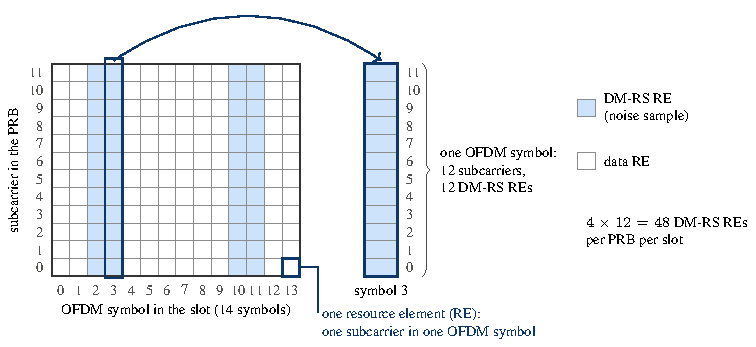
\includegraphics{Images/FLUXO/prb_dmrs.pdf}
\vspace{4pt}
\legend{Source: the author, with the DM-RS positions of \citesp{3gpp-ts38211}. \textcolor{red}{Double-symbol DM-RS}, mapping type~A, symbols 2, 3, 10 and 11.}
\end{figure}


A sample represents the noise covariance for a given data symbol only if both fall within the same interval of duration $T_c$. As a result, the number of available samples may vary from one data symbol to another. For any given symbol, the number of samples corresponds to the maximum count of DM-RS REs found within an interval of duration $T_c$ that encompasses that symbol. The number of samples available for all symbols in the slot is the smallest of these values. Figure~\ref{fig:dmrs-n} shows an example with the DM-RS located at symbols 2, 3, 10, and 11 of each slot. Under the TDLB100-400 condition, symbols 5 through 8 represent the worst-case scenario, with 24 samples. Therefore, the number of samples available for all symbols is 24. Table~\ref{tab:n-maximo} presents this value for each test condition.

\begin{table}[htbp]
\caption{Number of DM-RS REs per PRB available to every data symbol of the slot, in each test condition.}
\label{tab:n-maximo}
\vspace{4pt} % a classe zera o espaço entre a caption e a tabela
\centering
\footnotesize
\renewcommand{\arraystretch}{1.2}
\setlength{\aboverulesep}{0pt}
\setlength{\belowrulesep}{0pt}
\begin{tabular}{|c|c|c|c|c|}
\toprule
\multirow{2}{*}{\textbf{Test condition}} & \textbf{Frequency} & \multirow{2}{*}{{\boldmath $T_c$} \textbf{(ms)}} & \textbf{OFDM symbols} & \textbf{DM-RS REs} \\
 & \textbf{range} & & \textbf{in} {\boldmath $T_c$} & \textbf{available} \\
\midrule
TDLA30-5    & \multirow{2}{*}{FR1} & 25.0000 & 700 & 2400 \\
TDLA30-10   &                      & 12.5000 & 350 & 1200 \\
\cline{2-2}
TDLA30-75   & \multirow{2}{*}{FR2} & 1.6667  & 186 & 648 \\
TDLA30-300  &                      & 0.4167  & 46  & 168 \\
\cline{2-2}
TDLC300-100 & \multirow{4}{*}{FR1} & 1.2500  & 35  & 132 \\
TDLB100-400 &                      & 0.3125  & 8   & 24 \\
HST350      &                      & 0.0536  & \multirow{2}{*}{1} & \multirow{2}{*}{0} \\
HST500      &                      & 0.0375  &     &  \\
\bottomrule
\end{tabular}
\vspace{4pt}
\legend{Source: the author, from \citesp{3gpp-ts38104}; \citesp{3gpp-ts38211}; \citesp{tse-viswanath}. \textcolor{red}{Double-symbol DM-RS} in symbols 2, 3, 10 and 11, with every slot carrying PUSCH.}
\end{table}

The best range of a data symbol may include DM-RS that arrive after that symbol. In Figure ~\ref{fig:dmrs-n}(b), the best range of symbol 13 goes up to symbol 3 of the next slot. To use these samples, the receiver needs to store symbol 13 for 4 more symbols.
% Figura: de onde vem o N de uma condição de teste (2026-11-04).
%   (a) pior caso (símbolo 6) e (b) melhor caso (símbolo 13): as 8 posições de um
%       intervalo de T_c = 8 símbolos (TDLB100-400) que contêm o símbolo.
%   A antiga parte (a), o PRB em um slot, virou a Figura fig:prb-dmrs (fig-prb-dmrs.tex).
%   Contagens geradas em Python (DM-RS em {2,3,10,11}, slots contínuos, L = 8).
%   Cores repetidas de fig-prb-dmrs.tex, para a figura não depender da ordem.
\definecolor{dmrsfill}{HTML}{CDE2FB}
\definecolor{winblue}{HTML}{0D366B}
\definecolor{inksec}{HTML}{52514E}
\begin{figure}[htbp]
\caption{Intervals of duration $T_c$ that contain a data symbol, and their DM-RS REs per PRB, in the TDLB100-400 condition.}
\label{fig:dmrs-n}
\vspace{4pt} % a classe zera o espaço entre a caption e a figura
\centering
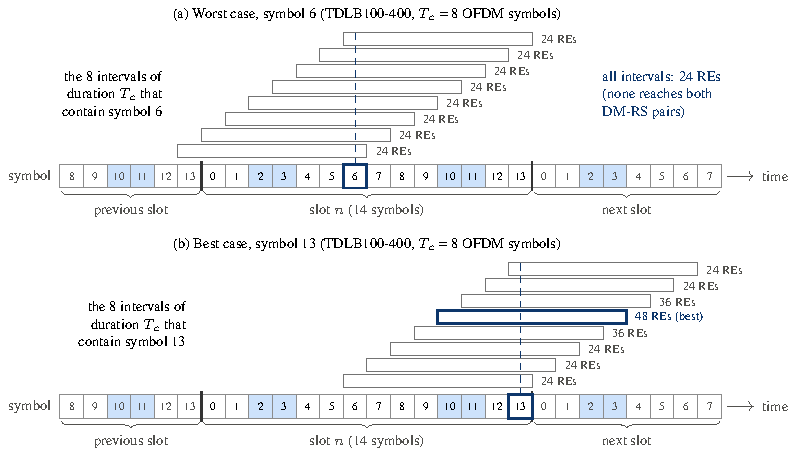
\includegraphics{Images/FLUXO/dmrs_n.pdf}
\vspace{4pt}
\legend{Source: the author, with the DM-RS positions of \citesp{3gpp-ts38211}. \textcolor{red}{Double-symbol DM-RS}, mapping type~A, symbols 2, 3, 10 and 11; continuous uplink. In (a) and (b), each bar is one position of an interval of duration $T_c$ that contains the marked symbol. Symbol 6 is the worst case of the slot, and symbol 13 is a best case.}
\end{figure}



\subsubsection{Condicionamento da estimativa}\label{subsubsec:condicionamento-R}
% ANTIGO:
% O posto de uma matriz é o número máximo de linhas ou colunas linearmente independentes que essa matriz possui.  Cada parcela $\mathbf{n}^i(\mathbf{n}^i)^H$ é uma matriz de posto unitário, uma vez que todas as suas colunas são múltiplas do mesmo vetor $\mathbf{n}^i$. Consequentemente, o posto da soma de (N) desses produtos é limitado por (N):
\textcolor{red}{O posto de uma matriz é o número máximo de linhas ou colunas linearmente independentes. Cada parcela $\mathbf{n}^i(\mathbf{n}^i)^H$ tem posto 1, porque todas as suas colunas são múltiplas de $\mathbf{n}^i$. Então, o posto da soma de $N$ parcelas é no máximo $N$:}

\[
\operatorname{rank}(\widehat{\mathbf R}_n) \leq \min(M,N)
\]

% ANTIGO:
% Assim, quando (N<M), a estimativa amostral da matriz completa $(M\times M)$ é necessariamente singular. Uma matriz singular não é inversível. Essa propriedade precisa ser considerada em operações que exigem a inversão da matriz de covariância.
%
% \cite{zhao2025jsac} adota a condição $N\gg K$, para obter uma estimativa suficientemente precisa. Em suas simulações, utiliza (N=192) amostras por realização do canal. Um trabalho anterior dos mesmos autores também apresenta 96 e 192 como valores típicos para essa quantidade de amostras (Zhao et al., 2021).
\textcolor{red}{Assim, quando $N<M$, $\widehat{\mathbf R}_n$ é singular e não tem inversa.}

\textcolor{red}{O artigo base adota $N\gg K$ para obter uma estimativa precisa e usa $N=192$ amostras por realização do canal \cite{zhao2025jsac}. Um trabalho anterior dos mesmos autores cita 96 e 192 como valores típicos \cite{zhao2021-globecom}.}

% SEPARAÇÃO (2026-11-04): explicação do Ledoit-Wolf trazida de METODOLOGIA/simulacao.tex.
\textcolor{red}{Uma forma de tornar a estimativa inversível é o encolhimento (\textit{shrinkage}) de Ledoit e Wolf. Ele troca $\hat{\mathbf R}_n$ por uma média ponderada entre $\hat{\mathbf R}_n$ e um múltiplo da identidade \cite{ledoit-wolf}:}
\begin{equation}
\hat{\mathbf R}_{\text{LW}}=(1-\textcolor{red}{\alpha})\,\hat{\mathbf R}_n+\textcolor{red}{\alpha}\,\mu\,\mathbf I_M,
\qquad
\mu=\frac{\operatorname{tr}(\hat{\mathbf R}_n)}{M}.
\label{eq:ledoit-wolf}
\end{equation}
\textcolor{red}{O peso $\alpha$, entre 0 e 1, é calculado a partir das próprias amostras, de forma a minimizar o erro quadrático esperado entre a estimativa e a covariância verdadeira \cite{ledoit-wolf}. Como $\hat{\mathbf R}_n$ não tem autovalores negativos, todo autovalor de $\hat{\mathbf R}_{\text{LW}}$ é pelo menos $\alpha\mu$. Quando $\alpha > 0$, a matriz resultante é inversível.}
% FONTE: Ledoit e Wolf (2004), alvo mu I com mu = tr/M e alpha estimado das amostras
%   (TODO: conferir número da equação/página). Simulador: m5_noise.shrink.
% NOSSO (conta): autovalores de (1-alpha)R + alpha mu I = (1-alpha) lambda_i + alpha mu >= alpha mu.
% FORA (sem fonte): a alternativa da carga diagonal com epsilon fixo.






% ---------------------------------------------------------------------
\subsection{Processamento descentralizado}\label{subsec:dbp}
% ---------------------------------------------------------------------

Na arquitetura descentralizada, as $M$ antenas da \sout{estação base} \textcolor{red}{BS} são particionadas em $C$ clusters, cada um associado a uma DU \textcolor{red}{(\textit{Distributed Unit}), uma unidade de processamento local \cite{zhao2025jsac}}. O vetor de ruído pode, então, ser organizado em componentes locais:

\[
\mathbf n=
\begin{bmatrix}
\mathbf n_1\\
\mathbf n_2\\
\vdots\\
\mathbf n_C
\end{bmatrix}.
\]

Essa partição induz uma estrutura em blocos na matriz de covariância $\mathbf R_n$. Os blocos diagonais $\mathbf R_{cc}$ descrevem a covariância do ruído observado pelas antenas do cluster $c$, enquanto os blocos fora da diagonal, $\mathbf R_{mn}$, representam as correlações entre antenas pertencentes a clusters distintos.

Cada DU dispõe localmente das amostras de ruído de suas próprias antenas. Assim, a DU $c$ pode estimar seu bloco diagonal sem trocar dados com as demais unidades:

\[
\hat{\mathbf R}_{cc}=
\frac{1}{N}
\sum_{i=1}^{N}
\mathbf n_c^i(\mathbf n_c^i)^H.
\]

Os blocos fora da diagonal, por outro lado, dependem de amostras provenientes de duas ou mais DUs. Sua estimação direta exige a troca de informações entre as unidades, aumentando o tráfego de comunicação.

Essa limitação estabelece uma relação entre as propriedades estatísticas do ruído e a estratégia de equalização descentralizada. 

% ---------------------------------------------------------------------
\subsection{Equalizador BCD-MMSE}\label{subsec:bcd}
% ---------------------------------------------------------------------



O equalizador BCD-MMSE \textcolor{red}{(\textit{Block Coordinate Descent}--\textit{Minimum Mean Square Error}) \cite{zhao2025jsac}}, por sua vez, emprega atualizações distribuídas para tratar o acoplamento entre os blocos do sistema, mantendo a necessidade de definir quais informações devem ser compartilhadas entre as unidades.

No BCD-MMSE considerado neste trabalho, a estimativa local $\hat{\mathbf R}_{cc}$ participa da inicialização do equalizador e da construção da matriz utilizada nas atualizações da DU. Em particular, a matriz local a ser invertida é definida por:

\[
\mathbf G_c=
E_s\mathbf H_c\mathbf H_c^H+
\hat{\mathbf R}_{cc},
\]

em que $\mathbf H_c$ representa a parcela da matriz de canal associada ao cluster $c$. Dessa forma, a estimação e o condicionamento da covariância local afetam diretamente a viabilidade das operações matriciais necessárias à equalização.

% SEPARAÇÃO (2026-11-04): propriedades do algoritmo trazidas do rascunho (Partes 1.3 e 1.4)
%   e de METODOLOGIA/simulacao.tex.
\textcolor{red}{A DU $c$ usa $\hat{\mathbf R}_{cc}$ de duas formas. Na inicialização, usa a inversa $\hat{\mathbf R}_{cc}^{-1}$, pois o BCD-MMSE começa pela aproximação bloco-diagonal \cite{zhao2025jsac}. Nas iterações, usa $\mathbf G_c$, que soma $\hat{\mathbf R}_{cc}$ ao termo do canal \cite{zhao2025jsac}. Assim, $\mathbf G_c$ usa $\hat{\mathbf R}_{cc}$, e não a sua inversa. Além disso, $\mathbf G_c$ não depende da iteração \cite{zhao2025jsac}. Ela é formada e invertida uma vez, e a inversa é usada em todas as iterações.}
% FONTE: Algoritmo 3, paper.md:415 (W^0 pela Eq. 7); Eq. 7, paper.md:136-142 (R_cc^-1);
%   Eq. 30, paper.md:504 (G_c sem índice de iteração).

\textcolor{red}{O número $N$ de amostras também tem um custo de armazenamento e de comunicação. Cada DU guarda as $N$ amostras de ruído das suas antenas \cite{zhao2025jsac}. Trocar essas amostras entre as DUs exigiria transferir dados de tamanho $M \times N$ \cite{zhao2025jsac}. No BCD-MMSE, a banda de comunicação em cada iteração também depende de $N$ \cite{zhao2025jsac}. Como a estimativa só muda a cada bloco de coerência, esse custo é pago uma vez a cada $N_{\text{coh}}$ símbolos \cite{zhao2025jsac}.}
% FONTE: paper.md:493 (N_c em C^{M_c x N} na DU c); :130 (M x N); :471 (banda por
%   iteração depende de N); :561 e :571 (termos divididos por N_coh).


\subsubsection{Complexidade}\label{subsubsec:bcd-complexidade}
\textcolor{red}{No artigo base, o pré-processamento de cada DU tem complexidade $\mathcal{O}(M_c^3 + N M_c^2)$, e cada iteração do BCD-MMSE tem complexidade $\mathcal{O}(NMK + M M_c K)$ no total \cite{zhao2025jsac}. A Tabela~\ref{tab:bcd-complexidade} mostra o número de multiplicações complexas de cada parte do algoritmo em uma DU, por PRB e por $T_c$. Várias partes dependem de $N$, que muda com a condição de teste (Tabela~\ref{tab:condicoes_teste}). Neste trabalho, só a inversa de $\mathbf G_c$ é calculada em ponto fixo (Seção~\ref{sec:simulador}).}

\begin{table}[htbp]
\caption{\textcolor{red}{Multiplicações complexas por PRB e por $T_c$ em cada DU.}}
\label{tab:bcd-complexidade}
\vspace{4pt} % a classe zera o espaço entre a caption e a tabela
\centering
\footnotesize
\renewcommand{\arraystretch}{1.2}
\setlength{\aboverulesep}{0pt}
\setlength{\belowrulesep}{0pt}
\begin{tabular}{|l|l|}
\toprule
\textbf{Parte} & \textbf{Multiplicações complexas} \\
\midrule
Estimar $\hat{\mathbf R}_{cc}$ e aplicar Ledoit-Wolf & $N M_c^2 + N M_c + M_c^2$ \\
\hline
Inicialização, com a inversa de $\hat{\mathbf R}_{cc}$ & $M_c^3 + M_c^2 K + M_c K^2 + 2K^2 M_c + N K M_c$ \\
\hline
Formar $\mathbf G_c$ & $M_c^2 K$ \\
\hline
Inverter $\mathbf G_c$ & $M_c^3$ \\
\hline
Cada iteração & $2NKM_c + 3K^2 M_c + K M_c^2$ \\
\hline
Inverter a matriz $K \times K$ (só na DU $C$) & $K^3$ \\
\hline
Filtro, por símbolo de dados & $12 K M_c$ \\
\bottomrule
\end{tabular}
\end{table}
% FONTE: software/Restrições - Parâmetros.csv, linhas 56-65 (modelo B).
%        Estimar R_cc: paper.md:554 (O(M_c^3 + N M_c^2) por DU). Inicialização (R_cc^-1, X_c, H_c^H X_c,
%        W_c^0, A^0, b^0): paper.md:136-142 (Eq. 7) e :410-418. G_c: paper.md:504. Iteração (Eqs. 28-30):
%        paper.md:556 (O(NMK + M M_c K) no total), :443-449, :504. Filtro: paper.md:430-434.
% 2026-11-09: tirados os valores numéricos (vários N) e a coluna dos módulos de inversão (só G_c
%        é invertida em ponto fixo). A inversão de R_cc (M_c^3) entrou na linha da inicialização.


% =====================================================================
\section{Inversão de Matrizes}\label{sec:inversao}
% =====================================================================
% ---------------------------------------------------------------------
\subsection{Inversao de Matrizes}\label{subsec:inversao}
% ---------------------------------------------------------------------

\subsubsection{Decomposicao de Cholesky}


% ---------------------------------------------------------------------
% SEPARAÇÃO (2026-11-04): conceitos trazidos do rascunho (Parte 1.5) e de
%   METODOLOGIA/requisitos-tempo.tex (vazão, latência e II).
% ---------------------------------------------------------------------
\subsubsection{\textcolor{red}{Representação em ponto fixo}}\label{subsubsec:ponto-fixo}
\textcolor{red}{Em hardware, os números costumam ser representados em ponto fixo. No Vitis HLS, o tipo \texttt{ap\_fixed}$\langle W, I\rangle$ tem $W$ bits no total, dos quais $I$ são da parte inteira \cite[p.~73--74]{kastner-hls}. A parte fracionária tem $F = W - I$ bits. Neste trabalho, o formato é escrito como $\langle W, I\rangle$.}

\textcolor{red}{Quando um valor não cabe na parte inteira, ocorre um estouro (\textit{overflow}). Uma forma comum de tratá-lo é descartar os bits mais significativos, o que se chama \textit{wrapping} \cite[p.~70]{kastner-hls}. Em complemento de dois, isso pode até trocar o sinal do número \cite[p.~71]{kastner-hls}. Quando um valor não cabe na parte fracionária, ele precisa ser arredondado \cite[p.~71]{kastner-hls}. Descartar os bits extras arredonda em direção a $-\infty$. Outras formas arredondam em direção a $+\infty$, em direção a zero, para longe de zero, ou para o valor mais próximo, com o empate indo para o valor par \cite[p.~71]{kastner-hls}.}

\textcolor{red}{O tipo \texttt{ap\_fixed} tem 7 modos de quantização e 5 modos de estouro, o que dá 35 combinações. A Tabela~\ref{tab:modos-apfixed} descreve cada um.} % TODO FONTE: UG1399.

\begin{table}[htbp]
\caption{\textcolor{red}{Modos de quantização e de estouro do tipo \texttt{ap\_fixed}.}}
\label{tab:modos-apfixed}
\centering
\footnotesize
\begin{tabular}{p{2.6cm}p{11cm}}
\toprule
Modo & Comportamento \\
\midrule
\multicolumn{2}{l}{\textit{Quantização (afeta os bits fracionários)}} \\
\texttt{AP\_TRN}       & Descarta os bits menos significativos. Arredonda em direção a $-\infty$. \\
\texttt{AP\_TRN\_ZERO} & Arredonda em direção a zero. Para números positivos, é igual ao \texttt{AP\_TRN}. \\
\texttt{AP\_RND}       & Arredonda para o valor mais próximo. No empate, arredonda em direção a $+\infty$. \\
\texttt{AP\_RND\_ZERO} & Arredonda para o valor mais próximo. No empate, arredonda em direção a zero. \\
\texttt{AP\_RND\_MIN\_INF} & Arredonda para o valor mais próximo. No empate, arredonda em direção a $-\infty$. \\
\texttt{AP\_RND\_INF}  & Arredonda para o valor mais próximo. No empate, afasta-se de zero. \\
\texttt{AP\_RND\_CONV} & Arredonda para o valor mais próximo. No empate, vai para o valor par. \\
\midrule
\multicolumn{2}{l}{\textit{Estouro (afeta os bits inteiros)}} \\
\texttt{AP\_SAT}       & Satura no maior ou no menor valor representável. \\
\texttt{AP\_SAT\_ZERO} & Em caso de estouro, o resultado vira zero. \\
\texttt{AP\_SAT\_SYM}  & Satura de forma simétrica: os limites positivo e negativo têm o mesmo módulo. \\
\texttt{AP\_WRAP}      & Descarta os bits mais significativos que não cabem (estouro em complemento de dois). \\
\texttt{AP\_WRAP\_SM}  & Faz o mesmo descarte, mas em sinal e magnitude. \\
\bottomrule
\end{tabular}
\legend{\textcolor{red}{Fonte: TODO (UG1399).}}
\end{table}
% ORIGEM: Análise bits.md, corrigido (AP_TRN_ZERO). Frases de custo de hardware dos
%   modos ficaram fora (sem fonte). Kastner et al. só tratam os conceitos, não os nomes
%   dos modos; para os nomes, a UG1399.

\subsubsection{\textcolor{red}{Latência, intervalo e vazão}}\label{subsubsec:latencia-intervalo}
\textcolor{red}{Em síntese de alto nível, uma tarefa é uma chamada de função. A latência da tarefa é o tempo entre o início e o fim de uma tarefa. O intervalo da tarefa é o tempo entre o início de uma tarefa e o início da seguinte \cite[p.~20]{kastner-hls}. Em um circuito com \textit{pipeline}, uma nova tarefa pode começar antes de a anterior terminar. Assim, o intervalo pode ser menor que a latência \cite[p.~21]{kastner-hls}. O intervalo entre dois dados que entram no \textit{pipeline} é chamado de intervalo de iniciação (II, \textit{Initiation Interval}) \cite[p.~21]{kastner-hls}.}

\textcolor{red}{No começo, o \textit{pipeline} está vazio, e só os primeiros estágios trabalham. O tempo até todos os estágios ficarem ocupados é o tempo de enchimento. No fim, o \textit{pipeline} também precisa esvaziar. Esse custo fixo pesa mais quando há poucas iterações \cite[pp.~114 e 146]{kastner-hls}.}

\textcolor{red}{Em uma sequência de tarefas, a primeira termina depois da latência $L$, e cada uma das seguintes, um intervalo $I$ depois da anterior. Assim, $n$ tarefas terminam em}
\begin{equation}\label{eq:fim-tarefas}
\textcolor{red}{t_n = L + (n-1)\, I.}
\end{equation}
% MOVIDO (2026-11-06) de METODOLOGIA/arquiteturas-hardware.tex (subseção "Pipeline e tempo de
%   enchimento"). Enchimento: redação própria; o livro não tem frase literal. Passagens:
%   p. 114 ("Once the pipeline is full, all four subfunctions are executing concurrently"),
%   p. 146 (esvaziamento; custo fixo em laços curtos). A Eq. sai das definições de latência
%   e intervalo (p. 20-21) e do exemplo da p. 45 (4 + (11-1)·1 = 14 ciclos).

\textcolor{red}{Muitas ferramentas chamam o intervalo de vazão (\textit{throughput}). Um intervalo maior quer dizer menos tarefas por unidade de tempo, ou seja, uma vazão menor \cite[p.~22]{kastner-hls}. Neste trabalho, a vazão é medida pelo intervalo entre inversões, e a latência é o tempo de uma inversão.}
% FONTE: Kastner et al. 2018 (books/Parallel Programming for FPGAs.pdf): p. 20
%   (task latency/interval), Fig. 1.7 p. 21 (pipelined: interval 1 < latency 10),
%   p. 21 (initiation interval), p. 22 (ferramentas chamam o intervalo de throughput).
% A CONFERIR: páginas contadas pelo PDF (páginas impressas iguais às do PDF neste livro).


\subsubsection{\textcolor{red}{Pipeline de tarefas}}\label{subsubsec:pipeline-tarefas}
\textcolor{red}{Uma tarefa pode ser dividida em etapas. No \textit{pipeline} de tarefas, as etapas trabalham ao mesmo tempo, cada uma em um dado diferente. Assim, a tarefa seguinte começa quando a anterior termina a primeira etapa. Em HLS, isso é feito com a diretiva \texttt{dataflow}, e cada etapa vira um processo separado. O intervalo do conjunto nunca é menor que o intervalo da etapa mais lenta \cite[pp.~113--115]{kastner-hls}.}
% FONTE: Kastner p. 113 ("different stages of the algorithm are operating on different data
%   sets. This optimization, called task pipelining is enabled using the dataflow directive"),
%   p. 114 (a segunda tarefa começa depois que a primeira termina a primeira função;
%   "pipeline stages (often called processes)"), p. 115 ("the achieved interval for the
%   overall pipeline can never be smaller than the interval of each individual process").

\subsubsection{\textcolor{red}{Arranjo sistólico}}\label{subsubsec:arranjo-sistolico}
\textcolor{red}{Um arranjo sistólico é um conjunto de elementos de processamento (PEs, \textit{processing elements}) iguais, em que cada PE só troca dados com os vizinhos. Esse tipo de projeto pode surgir quando um laço interno é desenrolado: cada cópia do corpo do laço vira um PE \cite[p.~180]{kastner-hls}.}
% FONTE: Kastner p. 180 (cópias do corpo do laço interno = "sorting cell"; cada célula só
%   se comunica com as vizinhas; "systolic arrays ... can naturally arise when we unroll inner
%   loops"); p. 153 (Processing Element, PE); glossário ("array of processing elements ...
%   only communicates with its local neighbors").

\textcolor{red}{A Figura~\ref{fig:sistolico-classico} mostra um arranjo sistólico em grade que calcula a matriz de Gram de $\mathbf H$. Como essa matriz é hermitiana, só o triângulo inferior é calculado. A cada ciclo, o arranjo lê uma linha de $\mathbf H$. Os dados entram por cima e pela esquerda e passam para o PE de baixo e para o da direita. Cada PE multiplica as duas entradas e acumula o produto. Depois de ler todas as linhas, cada PE guarda um elemento da matriz \cite[p.~2979]{wang2021tlbdinsa}.}
% FONTE: Wang et al. 2021 (referencias/hardware implementation/An_Efficient_Detector_for_
%   Massive_MIMO_Based_on_Improved_Matrix_Partition.pdf), p. 2979, Fig. 14 e texto: "Considering
%   A is Hermitian ... an M x M lower triangular systolic array (LTSA) ... reads the elements of
%   one-row matrix H at a time, and outputs the solution of the Gram matrix after N clock
%   cycles. Each processing element (PE) performs the multiply-accumulate (MAC)". Direção dos
%   dados (para baixo e para a direita) lida da Fig. 14.

\begin{figure}[!ht]
\caption{\textcolor{red}{Lower triangular systolic array that computes a Gram matrix.}}
\label{fig:sistolico-classico}
\vspace{4pt}
\centering
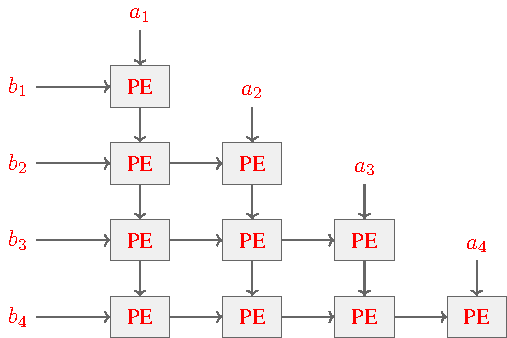
\includegraphics{Images/FLUXO/inversao_cholesky.pdf}
\vspace{4pt}
\legend{\textcolor{red}{Source: adapted from \citesp{wang2021tlbdinsa}, p.~2979. $a_j$ and $b_i$: elements of one row of $\mathbf H$, one row per cycle. Each PE multiplies $a_j$ by $b_i$, adds the product to its accumulator, and passes $a_j$ down and $b_i$ to the right.}}
\end{figure}

\chapter{Methodology}\label{chap:metodologia}
This chapter describes the tools used and the tests performed for this work. The uplink transmission of a massive MIMO system with decentralized processing (Section~\ref{subsec:uplink}) was simulated to analyze the effect of the approximation used in the inversion module of the BCD-MMSE algorithm. Based on this analysis, the fixed-point formats for the inversion module, implemented on an FPGA, are selected. The chapter begins by presenting the simulation workflow (Section~\ref{sec:simulador}) and the hardware tools (Section~\ref{sec:setup-hardware}). It then covers test configurations and conditions (Section~\ref{sec:configuracoes}), timing constraints for the inversion process (Section~\ref{sec:requisitos-tempo}), the selection of the numerical format (Section~\ref{sec:formato}), the hardware architectures, the matrices used to test them and the power estimation (Section~\ref{sec:testes-hardware}), and the organization of the results (Section~\ref{sec:organizacao-resultados}).



% =====================================================================
\section{\texorpdfstring{Simulation workflow}{Simulation workflow}}\label{sec:simulador}
% =====================================================================
The simulation workflow~\ref{fig:fluxo_simulacao} employs three tools: the QuaDRiGa channel generator, a Python simulator developed in this work, and C++ code developed in Vitis HLS, which computes the inverse of $\mathbf{G}_c$ using fixed-point arithmetic. QuaDRiGa generates the channel matrices $\mathbf{H}$ for the target UEs and $\overline{\mathbf{H}}$ for the interfering UEs.

The Python simulator handles the transmission process. It generates symbols for the target UEs and creates colored noise, with a covariance derived from $\overline{\mathbf{H}}$ (Section~\ref{subsec:ruido-colorido}), to construct the received signal using $\mathbf{H}$. Subsequently, it computes the equalizers, performs symbol detection, and measures the SER at various SNR levels. The BCD-MMSE algorithm is simulated in two ways: using the inverse of $\mathbf{G}_c$ in 64-bit floating-point format (which serves as a reference) and using the inverse in fixed-point format. In the latter case, whenever the BCD-MMSE algorithm requires $\mathbf{G}_c^{-1}$, the Python simulator invokes the C++ code.

The Python simulator models the same uplink as in \cite{zhao2025jsac}. According to the authors, that paper was the first work on decentralized processing to consider colored noise \cite{zhao2025jsac}. Therefore, the simulation parameters follow that work, except where the text indicates otherwise.



% Fluxo conferido no código:
%   QuaDRiGa: software/simulador/quadriga/export_quadriga_channels.m (semente: linha 83)
%   laço e equalizadores: dbp_sim/m1_driver.py:149-211; dbp_sim/m7_equalizers.py
%     (lmmse, zero_forcing, bdac_mmse, bcd_mmse_path); Ledoit-Wolf: dbp_sim/m5_noise.py:162-168
%   inversa em ponto fixo: dbp_sim/hls_inverse.py (usada nos resultados de SER,
%     varredura_formatos.py, bcd_inverse="hls") e dbp_sim/hw_inverse.py (modelo em Python)
% Conteúdo vem de constraints/diagramas/fluxo_simulador.puml; estrutura em caixas do
% rascunho constraints/diagramas/metodologia.svg.
\begin{figure}[!ht]
\caption{Simulation flow: QuaDRiGa channels, Python simulator and fixed-point inverse.}
\label{fig:fluxo_simulacao}
\vspace{4pt} % a classe zera o espaço entre a caption e a figura
\centering
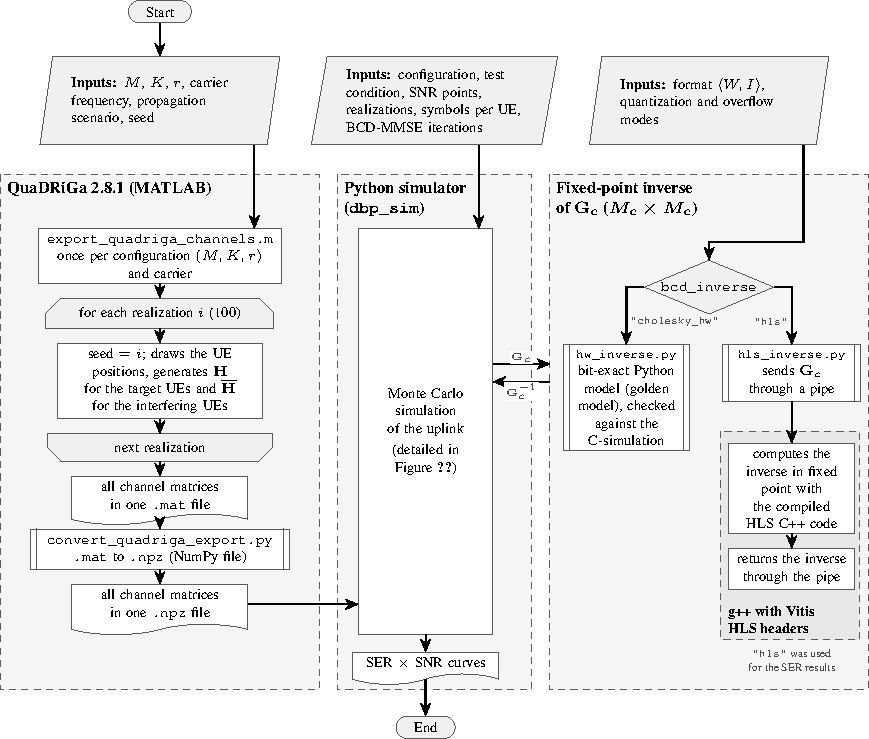
\includegraphics{Images/FLUXO/simulacao_a.pdf}
\vspace{4pt}
\legend{Source: the author.}
\end{figure}

% ---------------------------------------------------------------------
\subsection{\texorpdfstring{Channel generation}{Channel generation}}\label{subsec:simul-canal}
% ---------------------------------------------------------------------
The channels are generated using QuaDRiGa 2.8.1 in MATLAB. They depend on the number of antennas $M$, the number of target UEs $K$, the number of interfering UEs $r$, and the carrier frequency. Consequently, they are generated once for each combination of these values. Other parameters, such as $C$, the modulation scheme, and the IoTh, only affect the processing steps within the Python-based simulator. The simulation employs 100 channel realizations. Each realization consists of a random selection of UE positions, along with the corresponding channels $\mathbf{H}$ and $\overline{\mathbf{H}}$ generated by QuaDRiGa for those specific positions. Every realization uses its own unique random seed.


MATLAB saves the channels for all 100 realizations into a \texttt{.mat} file. A Python script then converts this file into an \texttt{.npz} file, NumPy’s format for storing multiple arrays within a single compressed file. The Python-based simulator reads the matrices $\mathbf{H}$ and $\overline{\mathbf{H}}$ from this file.
% ---------------------------------------------------------------------
\subsection{\texorpdfstring{Python simulator}{Python simulator}}\label{subsubsec:simul-python}
% ---------------------------------------------------------------------
The Python simulator runs two nested loops (Figure~\ref{fig:fluxo_python}). The outer loop iterates through the 100 realizations, while the inner loop iterates through the SNR points. The SNR points range from $-10$ to $10$~dB, with a step of $2$~dB. For each realization, the simulator takes $\mathbf{H}$ and $\overline{\mathbf{H}}$ corresponding to that realization and uses these channels across all SNR points. Each point on the SER curves represents the average over the 100 realizations. This is a Monte Carlo simulation, as in \cite{zhuang2025}: the SER (Section~\ref{subsubsec:ser}) is estimated by the fraction of erroneous symbols across many random draws of the channel, noise, and symbols.

At each SNR point, the simulator constructs the noise covariance matrix based on $\overline{\mathbf{H}}$, the IoTh (interference-over-thermal), and the SNR. It then generates $N$ noise samples, $\mathbf{n}^i$ (Section~\ref{subsubsec:estimacao-R}). It also generates 480 data symbols for each UE, along with the noise associated with these symbols. Based on this, the equalizers are calculated. The channel remains constant within the coherence block (Section~\ref{subsec:bloco-coerencia}); therefore, each equalizer is computed once and applied to all 480 symbols. The BCD-MMSE is compared against two centralized equalizers, the LMMSE and the ZF, which serve as benchmarks. The ZF does not utilize the noise samples $\mathbf{n}^i$. In contrast, both the LMMSE and the BCD-MMSE employ these samples to estimate the noise covariance (Section~\ref{subsubsec:condicionamento-R}). This estimate is always subjected to Ledoit-Wolf shrinkage (Equation~\ref{eq:ledoit-wolf}) before being used, even in cases where the estimate is already invertible.

In the LMMSE, this adjustment is applied to the estimate $\hat{\mathbf{R}}$ corresponding to all $M$ antennas. In the BCD-MMSE, each DU performs the adjustment on its own block, $\hat{\mathbf{R}}_{cc}$, using only the samples from its $M_c$ antennas. Consequently, no DU requires access to the samples from any other DU. The adjusted block forms the matrix $\mathbf{G}_c$ (Section~\ref{subsec:bcd}). In the reference version of the BCD-MMSE, this matrix is inverted using 64-bit floating-point arithmetic; alternatively, it can be inverted using fixed-point arithmetic (Section~\ref{subsubsec:simul-inversa}).



\begin{figure}[!ht]
\caption{Detailed flow of the Python simulator: Monte Carlo loop, equalizers and SER.}
\label{fig:fluxo_python}
\vspace{4pt} % a classe zera o espaço entre a caption e a figura
\centering
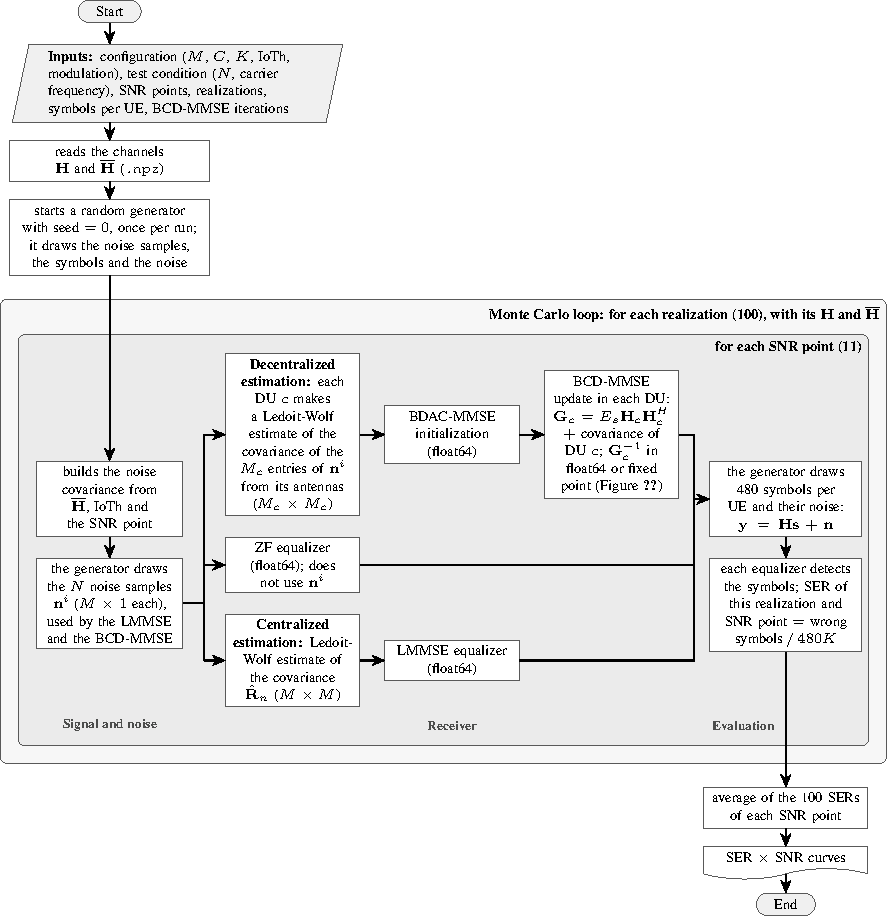
\includegraphics{Images/FLUXO/simulacao_b.pdf}
\vspace{4pt}
\legend{Source: the author.}
\end{figure}

% ---------------------------------------------------------------------
\subsection{\texorpdfstring{Fixed-point inverse}{Fixed-point inverse}}\label{subsubsec:simul-inversa}
% ---------------------------------------------------------------------
The inverse of $\mathbf{G}_c$ in fixed-point arithmetic is derived from the C++ code of the inversion module (Section~\ref{subsec:hw-modulo}). This code is compiled using \texttt{g++} along with the \texttt{ap\_fixed} header files from Vitis HLS 2026.1, with a separate compilation performed for each combination of format $\langle W, I\rangle$, quantization mode, overflow mode (Table~\ref{tab:modos-apfixed}), and size $M_c$. The program remains active throughout the simulation. Other calculations within the simulator, including the inverses used for BDAC initialization and LMMSE, utilize 64-bit floating-point arithmetic.

To verify this program, the same $\mathbf{G}_c$ matrices used in the simulator were inverted both by this program and by the Vitis HLS C-simulation. This process involved 30 matrices for each of the 35 mode combinations, with $M_c$ set to 16 and 32. In every instance, the resulting inverses were bit-identical. Consequently, the Symbol Error Rate (SER) is measured using the exact same inverse as that calculated by the hardware. The simulator also includes a Python-based model of the inversion, which has been verified bit-for-bit against the C++ code; however, the reported SER results are based on the C++ implementation.

% REMOVIDO (2026-11-05): subseção "Flow diagram". A Figura fig:fluxo_simulacao foi para a
%   abertura da seção; a frase da subseção ficou redundante com a abertura.



% =====================================================================
\section{\texorpdfstring{Hardware setup}{Hardware setup}}\label{sec:setup-hardware}
% =====================================================================
% =====================================================================
% SETUP DE HARDWARE (Metodologia) -- rascunho de 2026-11-04
% Ainda não incluído no METODOLOGIA.tex. Para incluir:
%   \section{Hardware Setup}\label{sec:setup-hardware}
%   % =====================================================================
% SETUP DE HARDWARE (Metodologia) -- rascunho de 2026-11-04
% Ainda não incluído no METODOLOGIA.tex. Para incluir:
%   \section{Hardware Setup}\label{sec:setup-hardware}
%   \input{chapters/METODOLOGIA/setup-hardware.tex}
% Fontes do projeto (conferidas em 2026-11-04):
%   hardware/pacote_servidor_formatos/{LEIAME.md, vivado.tcl, potencia.py, rodar.sh}
%   hardware/pacote_servidor_2023/LEIAME.md
%   hardware/testes/{AMOSTRAGEM.md, LEIAME.md}
%   hardware/cholesky_hardware/{hls_config_sintese_24_12*.cfg, tb_potencia.cpp}
%   hardware/cholesky_hardware_diretivas*/LEIAME.md; acompanhamento_experimentos.csv
% Nomes das configurações: mapa LETRAS de software/testes/mapa_cenarios_v4.py
%   (antigos 1-8 = 1A,1E,1B,1F,1C,1G,1D,1H; 9-12 = 2A,2E,2B,2F).
% =====================================================================

% ---------------------------------------------------------------------
\subsection{\texorpdfstring{Tools and target device}{Tools and target device}}\label{subsec:hw-ferramentas}
% ---------------------------------------------------------------------
The inversion module was described in C++ and synthesized in Vitis HLS 2026.1. Vitis HLS generates the module's RTL. Then, the RTL was synthesized, placed, and routed in Vivado 2023.2. The target device is the AMD Alveo U50 board, with the XCU50-FSVH2104-2-E FPGA. This FPGA has 5,952 DSP blocks and 871,680 LUTs. All circuits use a clock frequency of 100 MHz, or a period of 10 ns.

In Vivado, the inversion module is synthesized and implemented alone, as the top-level design, without any other surrounding board logic. The flow performs synthesis, optimization, placement, physical optimization, and routing. The only timing constraint is the clock period, and the paths entering and exiting the module's ports are not constrained. Thus, the resource, timing, and power figures for this work are only for the module and come from the routed design in Vivado 2023.2.

Before the Vivado workflow, each version went through the Vitis HLS C synthesis. A version only went to Vivado if the HLS estimate fit within the FPGA: a maximum of 5,952 DSP blocks and a maximum of 90\% of the LUTs.

% ---------------------------------------------------------------------
\subsection{\texorpdfstring{Inversion module}{Inversion module}}\label{subsec:hw-modulo}
% ---------------------------------------------------------------------
The module receives the $M_c \times M_c$ matrix $\mathbf{G}_c$ and returns its inverse. It calculates the inverse using Cholesky decomposition (Section~\ref{sec:inversao}). Two sizes for $\mathbf{G}_c$, corresponding to the configurations described in Section~\ref{subsec:configuracoes-bs}, have been implemented: $16 \times 16$ and $32 \times 32$. The input, output, and internal values use the \texttt{ap\_fixed} data type, following the formats selected in Section~\ref{sec:formato}.

The module consists of six stages, each implemented as a C++ function (Figure~\ref{fig:modulo-inversao}). These stages are executed sequentially, with each stage passing its output to the next.
\begin{figure}[!ht]
\caption{Steps of the inversion module. Each block is one C++ function of the HLS code.}
\label{fig:modulo-inversao}
\vspace{4pt} % a classe zera o espaço entre a caption e a figura
\centering
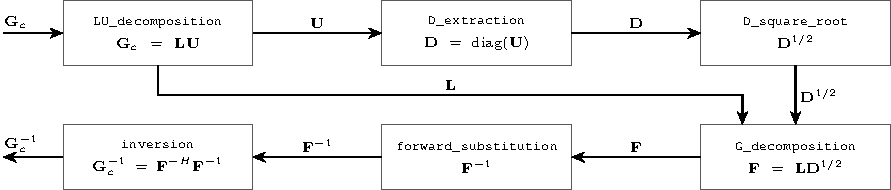
\includegraphics{Images/FLUXO/modulo_inversao.pdf}
\vspace{4pt}
\legend{Source: the author.}
\end{figure}

Additions, multiplications, and divisions utilize \texttt{ap\_fixed} type operators. Complex multiplication and division operations are explicitly implemented in the code, with a specific type defined for each intermediate value; thus, the bit-width of every intermediate value is explicitly set within the code. The addition of two $N$-bit numbers requires $N+1$ bits, while their product requires $2N$ bits \cite[pp.~72--73]{kastner-hls}. When using \texttt{ap\_fixed} types, the result of an operation inherently possesses a sufficient number of bits; overflow only occurs when this result is assigned to a type with a smaller bit-width \cite[p.~74]{kastner-hls}. Consequently, intermediate values employ types with greater bit-widths than the $\langle W, I\rangle$ format (Table~\ref{tab:tipos-intermediarios}), with the result reverting to the specified format only at the output of each stage. Square root calculations are performed using the \texttt{hls::sqrt} function from Vitis HLS, operating directly within the defined format.

\begin{table}[!ht]
\caption{Types of the values in the inversion module, for the format $\langle W, I\rangle$ with $F = W - I$ fractional bits.}
\label{tab:tipos-intermediarios}
\vspace{4pt} % a classe zera o espaço entre a caption e a tabela
\centering
\footnotesize
\renewcommand{\arraystretch}{1.2}
\begin{tabular}{p{7.4cm}cc}
\toprule
\textbf{Value} & \textbf{Integer bits} & \textbf{Fractional bits} \\
\midrule
Input, output and output of each step & $I$ & $F$ \\
Square root (\texttt{hls::sqrt}) & $I$ & $F$ \\
Accumulated sums, numerator and divisor of the complex division, quotient & $2I$ & $2F$ \\
Product of two real numbers & $4I$ & $4F$ \\
Real or imaginary part of a complex product (sum of two products) & $4I + 1$ & $4F$ \\
\bottomrule
\end{tabular}
\vspace{4pt}
\legend{Source: the author. The intermediate values use the same quantization and overflow modes as the format; the square root uses AP\_TRN and AP\_WRAP.}
\end{table}


% ---------------------------------------------------------------------

% Fontes do projeto (conferidas em 2026-11-04):
%   hardware/pacote_servidor_formatos/{LEIAME.md, vivado.tcl, potencia.py, rodar.sh}
%   hardware/pacote_servidor_2023/LEIAME.md
%   hardware/testes/{AMOSTRAGEM.md, LEIAME.md}
%   hardware/cholesky_hardware/{hls_config_sintese_24_12*.cfg, tb_potencia.cpp}
%   hardware/cholesky_hardware_diretivas*/LEIAME.md; acompanhamento_experimentos.csv
% Nomes das configurações: mapa LETRAS de software/testes/mapa_cenarios_v4.py
%   (antigos 1-8 = 1A,1E,1B,1F,1C,1G,1D,1H; 9-12 = 2A,2E,2B,2F).
% =====================================================================

% ---------------------------------------------------------------------
\subsection{\texorpdfstring{Tools and target device}{Tools and target device}}\label{subsec:hw-ferramentas}
% ---------------------------------------------------------------------
The inversion module was described in C++ and synthesized in Vitis HLS 2026.1. Vitis HLS generates the module's RTL. Then, the RTL was synthesized, placed, and routed in Vivado 2023.2. The target device is the AMD Alveo U50 board, with the XCU50-FSVH2104-2-E FPGA. This FPGA has 5,952 DSP blocks and 871,680 LUTs. All circuits use a clock frequency of 100 MHz, or a period of 10 ns.

In Vivado, the inversion module is synthesized and implemented alone, as the top-level design, without any other surrounding board logic. The flow performs synthesis, optimization, placement, physical optimization, and routing. The only timing constraint is the clock period, and the paths entering and exiting the module's ports are not constrained. Thus, the resource, timing, and power figures for this work are only for the module and come from the routed design in Vivado 2023.2.

Before the Vivado workflow, each version went through the Vitis HLS C synthesis. A version only went to Vivado if the HLS estimate fit within the FPGA: a maximum of 5,952 DSP blocks and a maximum of 90\% of the LUTs.

% ---------------------------------------------------------------------
\subsection{\texorpdfstring{Inversion module}{Inversion module}}\label{subsec:hw-modulo}
% ---------------------------------------------------------------------
The module receives the $M_c \times M_c$ matrix $\mathbf{G}_c$ and returns its inverse. It calculates the inverse using Cholesky decomposition (Section~\ref{sec:inversao}). Two sizes for $\mathbf{G}_c$, corresponding to the configurations described in Section~\ref{subsec:configuracoes-bs}, have been implemented: $16 \times 16$ and $32 \times 32$. The input, output, and internal values use the \texttt{ap\_fixed} data type, following the formats selected in Section~\ref{sec:formato}.

The module consists of six stages, each implemented as a C++ function (Figure~\ref{fig:modulo-inversao}). These stages are executed sequentially, with each stage passing its output to the next.
\begin{figure}[!ht]
\caption{Steps of the inversion module. Each block is one C++ function of the HLS code.}
\label{fig:modulo-inversao}
\vspace{4pt} % a classe zera o espaço entre a caption e a figura
\centering
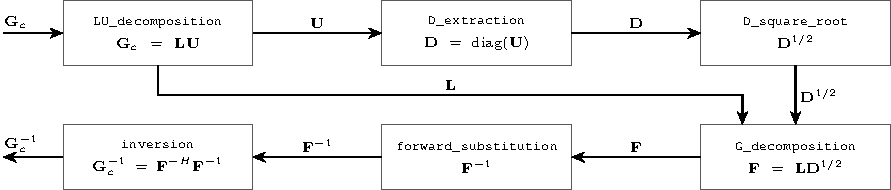
\includegraphics{Images/FLUXO/modulo_inversao.pdf}
\vspace{4pt}
\legend{Source: the author.}
\end{figure}

Additions, multiplications, and divisions utilize \texttt{ap\_fixed} type operators. Complex multiplication and division operations are explicitly implemented in the code, with a specific type defined for each intermediate value; thus, the bit-width of every intermediate value is explicitly set within the code. The addition of two $N$-bit numbers requires $N+1$ bits, while their product requires $2N$ bits \cite[pp.~72--73]{kastner-hls}. When using \texttt{ap\_fixed} types, the result of an operation inherently possesses a sufficient number of bits; overflow only occurs when this result is assigned to a type with a smaller bit-width \cite[p.~74]{kastner-hls}. Consequently, intermediate values employ types with greater bit-widths than the $\langle W, I\rangle$ format (Table~\ref{tab:tipos-intermediarios}), with the result reverting to the specified format only at the output of each stage. Square root calculations are performed using the \texttt{hls::sqrt} function from Vitis HLS, operating directly within the defined format.

\begin{table}[!ht]
\caption{Types of the values in the inversion module, for the format $\langle W, I\rangle$ with $F = W - I$ fractional bits.}
\label{tab:tipos-intermediarios}
\vspace{4pt} % a classe zera o espaço entre a caption e a tabela
\centering
\footnotesize
\renewcommand{\arraystretch}{1.2}
\begin{tabular}{p{7.4cm}cc}
\toprule
\textbf{Value} & \textbf{Integer bits} & \textbf{Fractional bits} \\
\midrule
Input, output and output of each step & $I$ & $F$ \\
Square root (\texttt{hls::sqrt}) & $I$ & $F$ \\
Accumulated sums, numerator and divisor of the complex division, quotient & $2I$ & $2F$ \\
Product of two real numbers & $4I$ & $4F$ \\
Real or imaginary part of a complex product (sum of two products) & $4I + 1$ & $4F$ \\
\bottomrule
\end{tabular}
\vspace{4pt}
\legend{Source: the author. The intermediate values use the same quantization and overflow modes as the format; the square root uses AP\_TRN and AP\_WRAP.}
\end{table}


% ---------------------------------------------------------------------


% =====================================================================
\section{\texorpdfstring{Configurations and test conditions}{Configurations and test conditions}}\label{sec:configuracoes}
% =====================================================================
\subsection{\texorpdfstring{Base station configurations}{Base station configurations}}\label{subsec:configuracoes-bs}
The uplink of the massive MIMO system was investigated using two types of parameters. Hard constraints refer to the physical characteristics of the base station: $M = 128$ or 256 antennas, $C = 8$ or 16 clusters, and the size $M_c = M/C$ of the inversion module. Soft constraints depend on the UEs being served and the level of interference: $K = 8$ or 12 UEs, QPSK or 16-QAM modulation, and an IoTh ratio of 10 dB as a baseline case, or 20 dB representing an extreme, high-interference scenario. These configurations were adapted from \cite{zhao2025jsac}. Table~\ref{tab:paineis} presents these configurations.


Each configuration is identified by a label consisting of a number and a letter. The number denotes the hard constraints: 1 for $M = 128$ and $C = 8$; 2 for $M = 256$ and $C = 8$; and 3 for $M = 256$ and $C = 16$. The letter indicates the soft constraints and remains consistent across all three groups.

\begin{table}[htbp]
\caption{Simulated configurations.}
\label{tab:paineis}
\vspace{4pt} % a classe zera o espaço entre a caption e a tabela
\centering
\footnotesize
\renewcommand{\arraystretch}{1.2}
% sem espaço em volta das linhas do booktabs, para as bordas verticais não terem falhas
\setlength{\aboverulesep}{0pt}
\setlength{\belowrulesep}{0pt}
\begin{tabular}{|c|c|c|c|c|c|c|}
\toprule
\multirow{2}{*}{\textbf{Configuration}} & \multicolumn{3}{c|}{\textbf{Hard constraints}} & \multicolumn{3}{c|}{\textbf{Soft constraints}} \\
\cline{2-7}
 & {\boldmath $M$} & {\boldmath $C$} & {\boldmath $M_c$} & \textbf{IoTh (dB)} & \textbf{Modulation} & {\boldmath $K$} \\
-- & \texttt{M} & \texttt{C} & -- & \texttt{iot\_db} & \texttt{modulation} & \texttt{K} \\
\midrule
1A & \multirow{8}{*}{128} & \multirow{8}{*}{8} & \multirow{8}{*}{16} & \multirow{4}{*}{10} & \multirow{2}{*}{16-QAM} & 8 \\
1B & & & & & & 12 \\
\cline{6-7}
1C & & & & & \multirow{2}{*}{QPSK} & 8 \\
1D & & & & & & 12 \\
\cline{5-7}
1E & & & & \multirow{4}{*}{20} & \multirow{2}{*}{16-QAM} & 8 \\
1F & & & & & & 12 \\
\cline{6-7}
1G & & & & & \multirow{2}{*}{QPSK} & 8 \\
1H & & & & & & 12 \\
\midrule
2A & \multirow{8}{*}{256} & \multirow{8}{*}{8} & \multirow{8}{*}{32} & \multirow{4}{*}{10} & \multirow{2}{*}{16-QAM} & 8 \\
2B & & & & & & 12 \\
\cline{6-7}
2C & & & & & \multirow{2}{*}{QPSK} & 8 \\
2D & & & & & & 12 \\
\cline{5-7}
2E & & & & \multirow{4}{*}{20} & \multirow{2}{*}{16-QAM} & 8 \\
2F & & & & & & 12 \\
\cline{6-7}
2G & & & & & \multirow{2}{*}{QPSK} & 8 \\
2H & & & & & & 12 \\
\midrule
3A & \multirow{8}{*}{256} & \multirow{8}{*}{16} & \multirow{8}{*}{16} & \multirow{4}{*}{10} & \multirow{2}{*}{16-QAM} & 8 \\
3B & & & & & & 12 \\
\cline{6-7}
3C & & & & & \multirow{2}{*}{QPSK} & 8 \\
3D & & & & & & 12 \\
\cline{5-7}
3E & & & & \multirow{4}{*}{20} & \multirow{2}{*}{16-QAM} & 8 \\
3F & & & & & & 12 \\
\cline{6-7}
3G & & & & & \multirow{2}{*}{QPSK} & 8 \\
3H & & & & & & 12 \\
\bottomrule
\end{tabular}

\vspace{4pt}
\legend{Source: 1A, 1B, 1C, 1E, 2A and 3A adapted from \citesp{zhao2025jsac}; the others, the author. $r = 8$ in all configurations. Second header row: field names of \texttt{Panel} in the code.}

\end{table}

% AUTORA (9-results.tex:245) -- parágrafo retirado do texto (tom); o conteúdo ficou em comentário.
% Configurações 1, 9, 13, 3, 2, 5 = painéis (a), (b), (c), (e), (f), (g) da Fig. 8 de Zhao et al.
% O painel (d) não aparece no artigo. Na configuração 3 (painel e), r = 8 foi
% mantido; L577 liga r a K, então r = 12 também seria defensável.




\subsection{Test conditions}\label{subsec:setup_condicoes}
% Criado em 2026-11-04 (reorganização pedida pela autora): junta o que define as condições
%   de teste. Origens: RESULTADOS/setup_simulacao.tex (subsubseção "Test Conditions", texto da
%   autora, e Tabela tab:condicoes_teste); METODOLOGIA/simulacao.tex (parágrafo do N);
%   METODOLOGIA/formato.tex (TDLA30-5 e TDLA30-10 com as mesmas curvas).

The simulated test conditions of Table~\ref{tab:n-maximo} define the carrier frequency and the number of noise samples in the Python simulator, as shown in Table~\ref{tab:condicoes_teste}. The simulation does not include a time axis, and the channel does not account for the Doppler effect, so only these two variables change between test conditions. A frequency of 3.5 GHz was used for FR1 conditions, within the n78 band (3300 to 3800 MHz, TDD), and 28 GHz was used for FR2 conditions, within the n257 band (26500 to 29500 MHz, TDD) \cite[Tabs.~5.2-1 and 5.2-2]{3gpp-ts38104}. In each realization, the channels at both frequencies use the same UE positions. % TODO: 3,5 GHz não tem fonte. Sugestão: citar uma referência que use 3,5 GHz como banda típica do 5G NR (ex.: livro 5G and Beyond), ou dizer só que é uma escolha deste trabalho.


\begin{table}[htbp]
\caption{Carrier frequency and number of noise samples in each test condition.}
\label{tab:condicoes_teste}
\vspace{4pt} % a classe zera o espaço entre a caption e a tabela
\centering
\footnotesize
\renewcommand{\arraystretch}{1.2}
\begin{tabular}{ccccc}
\toprule
\textbf{Test condition} & \textbf{\shortstack{Frequency\\range}} & \textbf{\shortstack{Carrier\\frequency (GHz)}} & \textbf{\shortstack{Noise\\samples {\boldmath $N$}}} & \textcolor{red}{\textbf{\shortstack{UE speed\\(km/h)}}} \\
\texttt{M1\_Driver.} & -- & \texttt{M1\_Driver.} & \texttt{M5\_Noise.} & -- \\
\texttt{test\_conditions} & & \texttt{test\_conditions} & \texttt{n\_noise\_samples} & \\
\midrule
TDLA30-5 & FR1 & 3.5 & 192 & \textcolor{red}{1.5} \\
TDLA30-10 & FR1 & 3.5 & 192 & \textcolor{red}{3.1} \\
TDLA30-75 & FR2 & 28 & 192 & \textcolor{red}{2.9} \\
TDLA30-300 & FR2 & 28 & 168 & \textcolor{red}{11.6} \\
TDLC300-100 & FR1 & 3.5 & 132 & \textcolor{red}{30.8} \\
TDLB100-400 & FR1 & 3.5 & 24 & \textcolor{red}{123.3} \\
\bottomrule
\end{tabular}

\vspace{4pt}
% FONTE (velocidade): v = f_D c / f_c, Tse e Viswanath p. 70; f_D de TS 38.104 Tab. G.2.2-1/G.2.2-2; antes na Tabela tab:tempo-coerencia (retirada).
\legend{Source: \citesp{3gpp-ts38104} and the author. \textcolor{red}{Speed from $v = f_D c/f_c$ \citesp{tse-viswanath}.}}
\end{table}

This work employs a double-symbol DM-RS, located at symbols 2, 3, 10, and 11 of each slot \cite[Tab.~6.4.1.1.3-4]{3gpp-ts38211}, as it enables the differentiation of DM-RS signals among $K = 8$ or 12 UEs (Section~\ref{subsubsec:disponibilidade-amostras}). The value of $N$ for each condition is taken from Table~\ref{tab:n-maximo}, with an upper limit of 192, the value used in \cite{zhao2025jsac}. This $N$ assumes that the receiver waits for samples arriving after the data symbol (Section~\ref{subsec:pipeline}). The HST350 and HST500 conditions were not simulated, as they correspond to $N = 0$.

TDLA30-5 and TDLA30-10 share the same carrier frequency and the same $N$ value. Consequently, they exhibit identical SER curves, and the simulations cover 5 distinct test conditions. The only difference between them lies in the inversion cycle limit (Section~\ref{subsec:restricao-vazao}).

The test conditions are grouped into two mobility profiles based on UE speed (Table~\ref{tab:condicoes_teste}). The low-mobility profile includes TDLA30-5, TDLA30-10, and TDLA30-75, with speeds up to 3.1 km/h. The high-mobility profile comprises TDLA30-300, TDLC300-100, and TDLB100-400, with speeds ranging from 11.6 to 123.3 km/h. The ITU-R uses 3 km/h for indoor and pedestrian users, and 30 and 120 km/h for users in vehicles \cite[Sec.~8.2 and Tab.~5]{itu-m2412}. In each profile, the fastest condition is the most demanding: it has the smallest $T_c$ and the smallest $N$. This condition is TDLA30-75 in the low-mobility profile and TDLB100-400 in the high-mobility profile.

% FONTE ITU: Rep. ITU-R M.2412-0, Sec. 8.2 (p. 16): Indoor Hotspot "stationary and pedestrian",
%   Dense Urban "pedestrian and vehicular", Rural "pedestrian, vehicular and high speed vehicular";
%   Tab. 5a (p. 20): indoor 3 km/h; Tab. 5b (p. 23): indoor 3 km/h, in-car 30 km/h;
%   Tab. 5c (p. 25): indoor 3 km/h, 120 km/h e 500 km/h. Arquivo: books/R-REP-M.2412-2017-PDF-E.pdf.


% =====================================================================
\section{\texorpdfstring{Inversion cycle limit}{Inversion cycle limit}}\label{sec:requisitos-tempo}
% =====================================================================
This section calculates, based on the coherence time, the maximum number of cycles between two inversions under each test condition.

% ---------------------------------------------------------------------
\subsection{\texorpdfstring{Sample collection}{Sample collection}}\label{subsec:pipeline}
% ---------------------------------------------------------------------
The receiver first collects the $N$ noise samples for each PRB. Some of these samples arrive only after the data symbol (Section~\ref{subsubsec:disponibilidade-amostras}). Therefore, this work assumes that the receiver buffers the data symbols until the $N$ samples have been received. Subsequently, it processes the samples and equalizes the buffered data. A new set of samples arrives every interval $T_c$, and the processing must keep pace with this rate.

% ---------------------------------------------------------------------
\subsection{Throughput}\label{subsec:restricao-vazao}
% ---------------------------------------------------------------------
The estimate $\hat{\mathbf R}_{cc}$ is unique per PRB within each interval $T_c$ (Section~\ref{subsubsec:disponibilidade-amostras}). The matrix $\mathbf G_c$ is inverted once and serves all iterations of the BCD-MMSE algorithm (Section~\ref{subsec:bcd}). Thus, each DU performs one inversion of $\mathbf G_c$ per PRB every $T_c$. With $N_{\text{PRB}}$ PRBs, this results in $N_{\text{PRB}}$ inversions per DU every $T_c$. This work uses $N_{\text{PRB}} = 275$, which is the worst-case scenario for 5G NR (Section~\ref{subsec:simbolos}).

To track data collection, the module needs to complete the $N_{\text{PRB}}$ inversions within $T_c$. Let $T_{\text{inv}}$ be the interval between the start of two inversions (Section~\ref{subsubsec:latencia-intervalo}). Then:
\begin{equation}
{T_{\text{inv}} \leq \frac{T_c}{N_{\text{PRB}}}.}
\label{eq:restriction-flow}
\end{equation}
With a clock speed of 100 MHz (Section~\ref{subsec:hw-ferramentas}), this limit is given in cycles, rounded down. Table~\ref{tab:limite-ciclos} shows the limit for each test condition.

\begin{table}[!ht]
\caption{Maximum interval between inversions in each test condition.}
\label{tab:limite-ciclos}
\vspace{4pt} % a classe zera o espaço entre a caption e a tabela
\centering
\footnotesize
\renewcommand{\arraystretch}{1.2}
\begin{tabular}{lccc}
\toprule
\textbf{Test condition} & {\boldmath $T_c$} \textbf{(ms)} & {\boldmath $T_c/N_{\text{PRB}}$} \textbf{(\textmu s)} & \textbf{Limit at 100 MHz (cycles)} \\
\midrule
TDLA30-5    & 25.0000 & 90.9091 & 9090 \\
TDLA30-10   & 12.5000 & 45.4545 & 4545 \\
TDLA30-75   & 1.6667  & 6.0606  & 606 \\
TDLA30-300  & 0.4167  & 1.5152  & 151 \\
TDLC300-100 & 1.2500  & 4.5455  & 454 \\
TDLB100-400 & 0.3125  & 1.1364  & 113 \\
\bottomrule
\end{tabular}
\vspace{4pt}
\legend{Source: the author. $T_c$ from Table~\ref{tab:n-maximo}; $N_{\text{PRB}} = 275$.}
\end{table}

The hardware architectures in this work aim to meet this throughput limit under each test condition. The following are outside the scope: the delay between the arrival of a data symbol and its equalization; the throughput of the links between the DUs; and the other matrix inversions required by the BCD-MMSE algorithm, which the simulator performs using floating-point arithmetic (Section~\ref{subsubsec:simul-inversa}). The delay encompasses both the time spent waiting for samples and the latency of each inversion (i.e., the time elapsed from the start to the completion of an inversion).


% =====================================================================
\section{\texorpdfstring{Selection of the fixed-point format}{Selection of the fixed-point format}}\label{sec:formato}
% =====================================================================
% ---------------------------------------------------------------------
% 1.5  ESCOLHA DO FORMATO DE PONTO FIXO          -> nova seção da Metodologia
% ---------------------------------------------------------------------
% ORIGEM: TCC/Análise bits.md (resumo da autora), com as correções de 2026-11-04:
%   nomes 1A-3D no lugar das letras A-P; IoTh; "condição de teste" no lugar de
%   "cenário"; critério de escolha lexicográfico (não a razão perda/ocupação);
%   5 formatos finais (não 3); AP_TRN_ZERO corrigido; tabela de velocidades
%   retirada (já está em FUNDAMENTACAO/modelo-de-canal.tex).

\subsection{\texorpdfstring{SNR increase}{SNR increase}}\label{subsec:aumento-snr}

To select the $\langle W, I\rangle$ format (Section~\ref{subsubsec:ponto-fixo}), the BCD-MMSE algorithm was simulated using both fixed-point and 64-bit floating-point matrix inversion. Only the inversion of $\mathbf G_c$ differs between the two simulations; however, the SNR and SER are measured for the entire uplink. Each format was evaluated based on the SNR increase, that is, the additional SNR required by the uplink to achieve an $\mathrm{SER} = 10^{-2}$ compared to the floating-point case. This increase corresponds to the horizontal distance between the two SER curves, which is the standard method for comparing two schemes \cite[p.~55]{tse-viswanath}.

% grade de SNR: params.M1_Driver.snr_db_grid (-10 a 10, passo 2); QPSK a partir de -20 dB:
%   curvas_qpsk_256 (grupos 2 e 3) e curvas_qpsk_128 (grupo 1), referencia_qpsk_256.py
\textcolor{red}{As curvas de SER foram simuladas de $-10$ a 10~dB, com passo de 2~dB. Com QPSK, a grade começa em $-20$~dB, porque algumas curvas já atingem $\mathrm{SER} = 10^{-2}$ antes de $-10$~dB: quase todas as do LMMSE no grupo 1 e todas as do LMMSE e do BCD-MMSE nos grupos 2 e 3.}

Two thresholds were employed. A 0.1~dB threshold represents a near-ideal format, where the SER curve is virtually identical to that of the floating-point implementation. A 3~dB threshold serves as the maximum acceptable increase. An increase of 3~dB is equivalent to doubling the power \cite[p.~73]{tse-viswanath}. Consequently, at this threshold, each UE would need to transmit with twice the energy per symbol to compensate for the error introduced by the matrix inversion (Section~\ref{subsec:snr}).



\subsection{\texorpdfstring{Initial sweep}{Initial sweep}}
The first stage involved varying the integer and fractional parts separately, while keeping the other part fixed (Table~\ref{tab:varredura-inicial}). Each size was tested across 35 combinations of quantization and overflow modes (Table~\ref{tab:modos-apfixed}), using the BCD-MMSE algorithm with both 1 and 4 iterations.

\begin{table}[htbp]
\caption{Sizes tested in the initial sweep.}
\label{tab:varredura-inicial}
\vspace{4pt} % a classe zera o espaço entre a caption e a tabela
\centering
\footnotesize
\renewcommand{\arraystretch}{1.2}
\begin{tabular}{lll}
\toprule
\textbf{Sweep} & \textbf{Integer bits} ({\boldmath $I$}) & \textbf{Fractional bits} ({\boldmath $F$}) \\
\midrule
Integer part & 6, 8, 10, 12, 14, 16, 20, 24, 32 & 32 \\
Fractional part & 14 & 4, 6, 8, 10, 12, 16, 20, 24, 32 \\
\bottomrule
\end{tabular}
\vspace{4pt}
\legend{Source: the author.}
\end{table}
% NOTA: 9 + 9 = 18 tamanhos, mas <46,14> (I = 14, F = 32) aparece nas duas
%   varreduras: 17 tamanhos por varredura de configuração e condição.

\subsection{\texorpdfstring{Configurations of the initial sweep}{Configurations of the initial sweep}}
The initial sweep utilized the 16 configurations for which the floating-point SER curve reaches $10^{-2}$ within the $-10$ to $10$ dB range. Running all of these across the 5 test conditions would have resulted in 80 cases, each involving 17 sizes and 35 mode combinations; therefore, only 5 configurations were selected.


The selection process relied on the $\mathbf{G}_c$ matrices at two SNR points surrounding the operating point (defined as $\mathrm{SER} = 10^{-2}$ in floating-point arithmetic). From each matrix, the largest absolute value between the real and imaginary parts of the elements was taken, since the circuit stores the two parts separately. This value is referred to here as the ``maximum $|$part$|$''. In each case, the 99th percentile of these values was used to ensure that the overall ranking would not be disproportionately influenced by a few outlier matrices. Larger elements necessitate a greater number of integer bits. Configurations 1G, 1H, 2E, and 2F contain the largest elements and are the most demanding, while configuration 1A contains the smallest elements and was used as a baseline (Table~\ref{tab:gc-ponto-operacao}).


These configurations also span the extremes of precision requirements. With a limited number of bits, the rounding error in matrix inversion increases with the condition number \cite[p.~1603]{osinsky2023}. When the smallest eigenvalue is very small, the matrix approaches a singular state, making the result more dependent on the fractional part (Section~\ref{subsubsec:ponto-fixo}). Configurations 2E and 2F exhibit the highest condition numbers (at the 99th percentile), whereas configuration 1A features the smallest eigenvalues (at the 1st percentile).


\begin{table}[htbp]
\caption{$\mathbf{G}_c$ at the operating point of the initial-sweep configurations.}
\label{tab:gc-ponto-operacao}
\vspace{4pt} % a classe zera o espaço entre a caption e a tabela
\centering
\footnotesize
\renewcommand{\arraystretch}{1.2}
\setlength{\tabcolsep}{4pt}
\begin{tabular}{ccccccccc}
\toprule
 & \multicolumn{2}{c}{\textbf{SNR (dB)}} & \multicolumn{2}{c}{\textbf{Largest} {\boldmath $|$}\textbf{part}{\boldmath $|$}} & \multicolumn{2}{c}{\textbf{Condition number}} & \multicolumn{2}{c}{\textbf{Smallest eigenvalue}} \\
\cmidrule(lr){2-3}\cmidrule(lr){4-5}\cmidrule(lr){6-7}\cmidrule(lr){8-9}
\textbf{Configuration} & \textbf{192; 3.5} & \textbf{168; 28} & \textbf{192; 3.5} & \textbf{168; 28} & \textbf{192; 3.5} & \textbf{168; 28} & \textbf{192; 3.5} & \textbf{168; 28} \\
\midrule
1A & $-2.6$ & $-2.4$ & 63   & 66   & 57  & 58  & 1.9  & 1.9 \\
1G & $-9.3$ & $-9.1$ & 2266 & 2383 & 187 & 169 & 22.4 & 24.1 \\
1H & $-8.7$ & $-8.6$ & 2470 & 2385 & 195 & 172 & 22.1 & 24.7 \\
2E & $-5.8$ & $-5.6$ & 962  & 999  & 286 & 254 & 8.8  & 9.7 \\
2F & $-5.6$ & $-5.5$ & 983  & 987  & 282 & 285 & 8.8  & 9.5 \\
\bottomrule
\end{tabular}
\vspace{4pt}
\legend{Source: the author. Subcolumns: $N$; carrier in GHz.}

\end{table}

\subsection{\texorpdfstring{Synthesis and selection of formats for validation}{Synthesis and selection of formats for validation}}

The sizes and modes of the initial sweep were also synthesized in Vitis HLS to measure resource occupancy (LUT, DSP, FF, and BRAM). The occupancy of each circuit is that of the most used resource in the FPGA. In each configuration and test condition, the integer and fractional parts with the lowest occupancy were chosen, with an SNR increase of up to 3 dB and of up to 0.1 dB, in 1 and in 4 iterations. Combining the two parts resulted in 10 formats (Table~\ref{tab:formatos-origem}).


\begin{table}[htbp]
\caption{Configurations in which each format was chosen in the initial sweep.}
\label{tab:formatos-origem}
\vspace{4pt} % a classe zera o espaço entre a caption e a tabela
\centering
\footnotesize
\renewcommand{\arraystretch}{1.2}
\begin{tabular}{ccccc}
\toprule
 & \multicolumn{2}{c}{\textbf{1 iteration}} & \multicolumn{2}{c}{\textbf{4 iterations}} \\
\cmidrule(lr){2-3}\cmidrule(lr){4-5}
\textbf{Format} & \textbf{Up to 3~dB} & \textbf{Up to 0.1~dB} & \textbf{Up to 3~dB} & \textbf{Up to 0.1~dB} \\
\midrule
$\langle 14,6\rangle$  & 1A         & --                       & --             & --                       \\
$\langle 16,6\rangle$  & --         & --                       & 1A             & --                       \\
$\langle 18,8\rangle$  & --         & 1A                       & --             & --                       \\
$\langle 20,8\rangle$  & --         & --                       & --             & 1A                       \\
$\langle 22,12\rangle$ & 1H, 2E, 2F & --                       & --             & --                       \\
$\langle 24,12\rangle$ & 1G         & 2E, 2F                   & 1G, 1H, 2E, 2F & --                       \\
$\langle 26,12\rangle$ & --         & 1G$^{a}$, 1H$^{a}$       & --             & 2E, 2F                   \\
$\langle 28,12\rangle$ & --         & --                       & --             & 1G$^{a}$, 1H$^{a}$       \\
$\langle 28,14\rangle$ & --         & 1G$^{b}$, 1H$^{b}$       & --             & --                       \\
$\langle 30,14\rangle$ & --         & --                       & --             & 1G$^{b}$, 1H$^{b}$       \\
\bottomrule
\end{tabular}
\vspace{4pt}
\legend{Source: the author. Columns: SNR increase. No mark: all 5 test conditions. $^{a}$Only TDLB100-400. $^{b}$The other 4 conditions.}
\end{table}



\subsection{\texorpdfstring{Validation}{Validation}}\label{subsec:validacao}
The initial sweep fixed one part of the word while varying the other, and used only 5 configurations. This can change the most used resource and the best mode. Therefore, the 10 formats were simulated again, with the 35 mode combinations, in the 24 configurations and 5 test conditions.

In this step, BCD-MMSE used only 1 iteration. The 4 iterations of the initial sweep had already helped to choose the formats of the most demanding cases: $\langle 16,6\rangle$, $\langle 20,8\rangle$, $\langle 28,12\rangle$ and $\langle 30,14\rangle$ only appeared with 4 iterations (Table~\ref{tab:formatos-origem}). With 1 iteration, BCD-MMSE already has a good result in SER. Furthermore, the inverse of $\mathbf G_c$ is calculated once and used in all iterations, so the number of inversions does not change (Section~\ref{subsec:bcd}).

The circuit has only one mode. Therefore, each format received a fixed mode in each group of configurations (Section~\ref{sec:configuracoes}). All configurations in a group use the same circuit. The mode was chosen according to the following criteria, in this order:

\begin{enumerate}

\item the mode that leaves more pairs (configuration, test condition) with an increase in SNR of up to 3~dB. A pair that does not reach $\mathrm{SER} = 10^{-2}$ counts as out of bounds;
\item the lowest resource occupancy, by the most used resource in the synthesis;
\item  the quantization \texttt{AP\_RND\_ZERO}, which never uses more resources than the other tied modes;

\item the smallest increase in SNR in the worst pair;
\item the order of the modes in the list.

\end{enumerate}

% FONTE: grade curta = varredura_formatos.grade_perto (--snr-perto, extra_direita 2), [4] v4 e
%   v5; grade inteira = rodadas [5] (modo_fixo_3dB, _iot10, _qpsk_128, _qpsk_256) e
%   rodada6_mapa_grade_inteira.sh (modo_fixo_mapa, 2026-11-08), semente 0 como a referência.
\textcolor{red}{Nessa etapa, a simulação em ponto fixo usou só as SNRs em volta do ponto de operação, com passo de 2~dB. Elas começam no ponto da grade logo abaixo da SNR em que o BCD-MMSE em ponto flutuante atinge $\mathrm{SER} = 10^{-2}$ e vão de 4 a 7~dB além dela. Depois de escolhido o modo fixo, cada formato foi simulado de novo, só com esse modo, na grade inteira de SNR (Seção~\ref{subsec:aumento-snr}). Essas simulações usam a mesma semente da simulação em ponto flutuante. A escolha dos três formatos de cada grupo e os resultados da Seção~\ref{sec:resultados-formato} vêm delas.}

% ANTIGO: Then, with the fixed mode, three formats were chosen in each group. The first is the smallest format in which all configurations and conditions of the group reach $\mathrm{SER} = 10^{-2}$, with any increase in SNR. The second and third are the smallest, where all reach this point with an increase of up to 3 dB and up to 0.1 dB, respectively. These formats were implemented in Vivado and are in the Section \ref{sec:resultados-formato}.
\textcolor{red}{Depois, com o modo fixo, foram escolhidos dois formatos em cada grupo: o menor em que todas as configurações e condições do grupo atingem $\mathrm{SER} = 10^{-2}$ com aumento de SNR de até 3~dB, e o menor com aumento de até 0,1~dB. O aumento é arredondado em duas casas decimais. O menor formato que só atinge $\mathrm{SER} = 10^{-2}$, com qualquer aumento, não foi usado como critério, porque esse aumento chega a mais de 10~dB (Seção~\ref{sec:resultados-formato}). Esses formatos foram implementados no Vivado e estão na Seção~\ref{sec:resultados-formato}.}

% =====================================================================
\section{\texorpdfstring{Hardware architectures, test matrices and power}{Hardware architectures, test matrices and power}}\label{sec:testes-hardware}
% =====================================================================
% Separado de setup-hardware.tex em 2026-11-04: as ferramentas e o módulo ficam antes
%   (ferramentas); as arquiteturas, as matrizes de teste e a potência vêm depois do formato.
The chosen formats were synthesized using Vitis HLS. In all versions, the automatic loop pipelining feature was disabled \cite[p.~42]{ug1399}. The first version, without loop optimizations, was implemented for both $16 \times 16$ and $32 \times 32$ matrix sizes. In this version, the iterations of each loop execute sequentially, and the $N_{\text{PRB}} = 275$ matrices within a block are inverted one by one. Consequently, the interval between inversions exceeds the limits defined for all test conditions (Table~\ref{tab:limite-ciclos}), and the module does not track the arrival of the matrices at each $T_c$.

To meet the cycle limits for each test condition, a specific architecture was developed for every case, only in $16 \times 16$, with Vitis HLS directives that reduce the interval between inversions. All versions were implemented in Vivado, tested using $\mathbf G_c$ matrices obtained from the simulator (Section~\ref{subsec:hw-matrizes}), and evaluated for power consumption and energy per inversion (Section~\ref{subsec:hw-potencia}). Each version produces the same inverse as the non-optimized implementation, a result verified bit-for-bit against the C-language code.
% FONTE: hardware/viabilidade_32x32/LEIAME.md (síntese C, HLS 2026.1 local, 2026-11-02, <24,12>).
\textcolor{red}{As arquiteturas otimizadas não foram implementadas em $32 \times 32$. Uma síntese C de teste das seis, em $32 \times 32$ e no formato $\langle 24,12\rangle$, estimou intervalos acima do limite de ciclos de todas as condições de teste. Nas sistólicas, o intervalo cresce 4 vezes, com o quadrado do tamanho da matriz. A da TDLB100-400 também não caberia no FPGA. Para atender os limites em $32 \times 32$, seria preciso outra arquitetura, com mais área, e isso não foi testado.}

\subsection{\texorpdfstring{Hardware architectures}{Hardware architectures}}\label{subsec:hw-arquiteturas}
% ---------------------------------------------------------------------
All optimized architectures employ pipelining (Section~\ref{subsubsec:latencia-intervalo}). Every $T_c$, the DU inverts 275 matrices $\mathbf G_c$, one for each PRB (Section~\ref{sec:requisitos-tempo}). For the 9,090 and 4,545-cycle limits, the module inverts one matrix at a time. For tighter limits, it inverts the matrices in batches of $n$. In all cases, the module must receive the 275 matrices for a given block within the duration $T_c$.

The matrices within a batch are independent of one another. Consequently, $c$ of these matrices are computed in the same cycle using loop unrolling, which creates a copy of the loop body for each iteration. The loop that iterates over the $c$ matrices is nested within a pipelined loop, and the HLS tool performs the unrolling automatically \cite[pp.~41, 372, and 428]{ug1399}. When $c$ is less than $n$, groups of $c$ matrices are processed in alternating cycles. Each copy has its own dedicated memory bank, though it may share operators with the others.

The values for $n$ and $c$ were determined through trial and error and are presented in Table~\ref{tab:hw-arquiteturas}.
 

\begin{table}[htbp]
\caption{Batch of the inversion module in each test condition.}
\label{tab:hw-arquiteturas}
\vspace{4pt} % a classe zera o espaço entre a caption e a tabela
\centering
\footnotesize

\renewcommand{\arraystretch}{1.2}
\setlength{\tabcolsep}{4pt}
\begin{tabular}{lcccc}
\toprule
\textbf{Test condition} & \begin{tabular}[c]{@{}c@{}}\textbf{Limit per}\\\textbf{matrix (cycles)}\end{tabular} & \begin{tabular}[c]{@{}c@{}}\textbf{Matrices per}\\\textbf{batch} ({\boldmath $n$})\end{tabular} & \begin{tabular}[c]{@{}c@{}}\textbf{Copies}\\({\boldmath $c$})\end{tabular} & \begin{tabular}[c]{@{}c@{}}\textbf{Batches}\\\textbf{per block}\end{tabular} \\
\midrule
Without optimizations & --    & 1  & 1 & 275 \\
TDLA30-5    & 9090 & 1  & 1 & 275 \\
TDLA30-10   & 4545 & 1  & 1 & 275 \\
TDLA30-75   & 606   & 12 & 6 & 23 \\
TDLC300-100 & 454   & 16 & 8 & 18 \\
TDLA30-300  & 151   & 32 & 2 & 9 \\
TDLB100-400 & 113   & 32 & 4 & 9 \\
\bottomrule
\end{tabular}

\vspace{4pt}
\legend{Source: the author. Limit per matrix from Table~\ref{tab:limite-ciclos}.}
\end{table}



% ---------------------------------------------------------------------
\subsubsection{\texorpdfstring{Loop pipelining}{Loop pipelining}}\label{subsubsec:hw-pipeline-lacos}

The module consists of six sequential stages (Figure~\ref{fig:modulo-inversao}): LU decomposition, extraction of the diagonal $\mathbf D$, calculation of the square root $\mathbf D^{1/2}$, computation of $\mathbf F$, forward substitution, and inversion. For the 9,090-cycle limit, the internal loops of these stages are annotated with the \texttt{\#pragma HLS pipeline II=1} directive. The \texttt{D\_extraction} stage is the only one without this directive, as it merely copies the diagonal from $\mathbf U$ to $\mathbf D$ and requires significantly fewer cycles than the other stages.

This directive enables loop pipelining, specifying that a new iteration should begin every cycle, that is, an initiation interval (II) of 1 cycle (Section~\ref{subsubsec:latencia-intervalo}). If data dependencies or resource constraints prevent this, the HLS tool will automatically use a larger II \cite[p.~45]{kastner-hls}.

Figure~\ref{fig:hw-pipeline-lacos} illustrates a loop from the LU decomposition process, both without and with pipelining. The individual stages and loops for a given matrix are executed sequentially. Consequently, the next inversion process cannot begin until the current one has finished; in this case, the interval between inversions is equal to the latency \cite[p.~114]{kastner-hls}.

\begin{figure}[!ht]
\caption{Loop pipelining in the LU decomposition. The code is simplified.}
\label{fig:hw-pipeline-lacos}
\vspace{4pt} % a classe zera o espaço entre a caption e a figura
\centering
\begin{minipage}[c]{0.62\textwidth}
\fontsize{8}{9.6}\selectfont
\begin{verbatim}
for (line = column + 1; line < n; line++)
  for (k = column; k < n; k++) {
#pragma HLS pipeline II=1
    t = L[line][column] * U[column][k];
    U[line][k] = U[line][k] - t;
  }
\end{verbatim}
\end{minipage}

\vspace{8pt}
\begin{minipage}[c]{\textwidth}
\centering
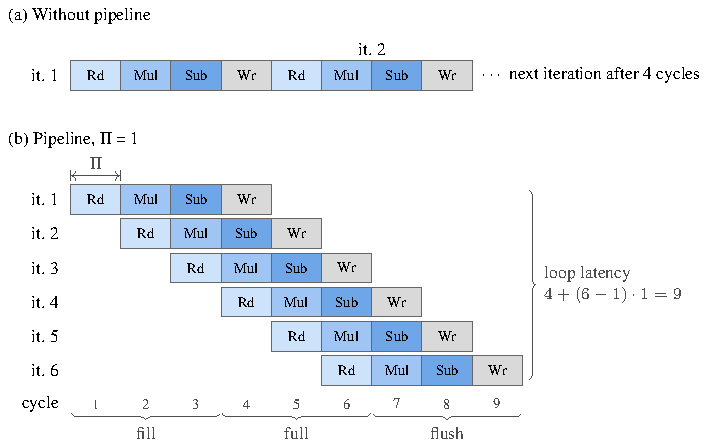
\includegraphics{Images/FLUXO/hw_pipeline_lacos.pdf}
\end{minipage}
\vspace{4pt}
\legend{Source: the author. Rd: read, Mul: multiply, Sub: subtract, Wr: write. Iteration latency of 4 cycles, for illustration.}
\end{figure}

% ---------------------------------------------------------------------
\subsubsection{\texorpdfstring{Dataflow between stages}{Dataflow between stages}}\label{subsubsec:hw-dataflow}

The architecture of the 4,545-cycle limit maintains the loop pipeline and combines the six steps into four: LU decomposition, calculation of $\mathbf F$ (\texttt{D\_extraction}, \texttt{D\_square\_root} and \texttt{G\_decomposition}), forward substitution, and inversion. The \texttt{\#pragma HLS dataflow} directive, applied to the top-level function, implements a task-level pipeline across the four stages, with each stage assigned to a specific matrix (Section~\ref{subsubsec:pipeline-tarefas}). Each step carries the directive \texttt{\#pragma HLS inline off}, which keeps it as a separate function \cite[p.~52]{kastner-hls}. In Figure~\ref{fig:hw-dataflow}, the latency of a matrix is the sum of the four steps, and the interval is the duration of the longest step.

% FONTE: cholesky_hardware_diretivas_4545/cholesky_top.cpp (etapa_lu, etapa_g, etapa_fs,
%   etapa_inv; dataflow em cholesky_inverse, linha 68). Kastner p. 52 (inline off mantém a
%   hierarquia), p. 114 (dataflow: as funções executam ao mesmo tempo, em dados diferentes).
%   Intervalo = etapa mais longa: Kastner p. 115 (na Fundamentação).

\begin{figure}[!ht]
\caption{Dataflow between the stages of the inversion. The code is simplified.}
\label{fig:hw-dataflow}
\vspace{4pt}
\centering
\begin{minipage}[c]{0.45\textwidth}
\fontsize{8}{9.6}\selectfont
\begin{verbatim}
void cholesky_inverse(A, inverse) {
#pragma HLS dataflow
  etapa_lu(A, L, U);
  etapa_g(U, L, G);
  etapa_fs(G, G_inv);
  etapa_inv(G_inv, inverse);
}

static void etapa_fs(G, G_inv) {
#pragma HLS inline off
  forward_substitution(G, G_inv);
}
\end{verbatim}
\end{minipage}

\vspace{8pt}
\begin{minipage}[c]{\textwidth}
\centering
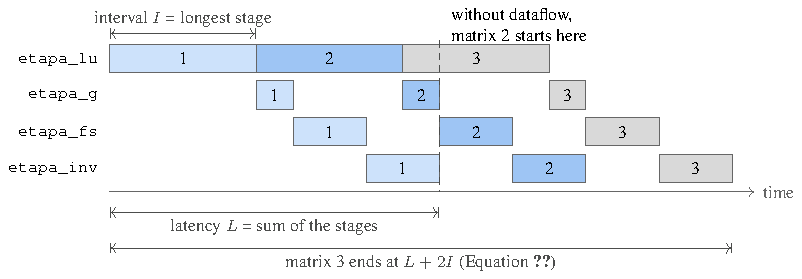
\includegraphics{Images/FLUXO/hw_c2.pdf}
\end{minipage}
\vspace{4pt}
\legend{Source: the author. Numbers in the boxes: index of the matrix.}
\end{figure}

% ---------------------------------------------------------------------
\subsubsection{\texorpdfstring{Matrix batches}{Matrix batches}}\label{subsubsec:hw-lotes}


Within the 606 and 454 cycle limits, the steps form a dataflow, as in the 4,545 cycle limit. The $c$ copies read different matrices in the same cycle, but a BRAM memory only allows access to two addresses per cycle. Therefore, the batch memory is divided into $c$ BRAM banks, one per copy, using the directive \texttt{\#pragma HLS array\_partition cyclic} and factor $c$. Thus, matrix $m$ is located in bank $m \bmod c$ \cite[pp.~87--88]{kastner-hls}.

Figure~\ref{fig:hw-lotes} shows the architecture of the 606 cycle limit. Since the two groups of 6 matrices alternate in each cycle, one iteration does not wait for the result of the previous one. Each copy has its own multipliers, but there is a single divider in each step, shared by the copies. It receives one matrix of the batch per cycle and, since it has a pipeline, it also does not wait for the previous division.

\begin{figure}[!ht]
\caption{Batch of 12 matrices with 6 copies, for the 606-cycle limit. The code is simplified.}
\label{fig:hw-lotes}
\vspace{4pt}
\centering
\begin{minipage}[c]{0.62\textwidth}
\fontsize{8}{9.6}\selectfont
\begin{verbatim}
#pragma HLS array_partition variable=U \
                     cyclic factor=COPIES dim=1
for (k = column; k < n; k++)
  for (g = 0; g < GRUPOS; g++) {
#pragma HLS pipeline II=1
    for (p = 0; p < COPIES; p++) {
      m = g * COPIES + p;
      t = L[m][line][column] * U[m][column][k];
      U[m][line][k] = U[m][line][k] - t;
    }
  }
\end{verbatim}
\end{minipage}

\vspace{8pt}
\begin{minipage}[c]{\textwidth}
\centering
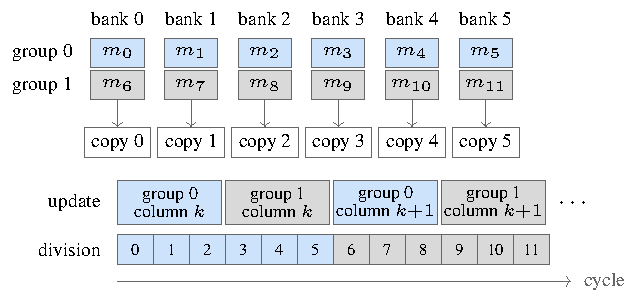
\includegraphics{Images/FLUXO/hw_c3.pdf}
\end{minipage}
\vspace{4pt}
\legend{Source: the author. Bank $p$ holds the matrices with $m \bmod 6 = p$. Update: 6 matrices per cycle. Division: one matrix $m$ per cycle, in a single divider.}
\end{figure}

% ---------------------------------------------------------------------
\subsubsection{\texorpdfstring{Systolic arrays}{Systolic arrays}}\label{subsubsec:hw-sistolico}

Within the 151 and 113-cycle limits, the stages also form a dataflow, with each copy featuring its own divider. LU decomposition, forward substitution, and inversion utilize systolic arrays: the $k$-loop, which iterates over a row or a summation, is nested within a pipelined loop, which HLS unrolls into 16 processing elements (PEs) (Section~\ref{subsubsec:arranjo-sistolico}). Each stage employs an array structure per copy, resulting in a total of $3c$ such arrays within the module.

In forward substitution and inversion, each PE adds a term and passes the partial sum to the next PE, following the same sequence as the unoptimized version, with each cycle computing a complete sum. In the LU decomposition, each cycle updates an entire row, with one element assigned to each PE. To achieve this, each row element is stored in its own dedicated register, configured using the \texttt{\#pragma HLS array\_partition complete} directive \cite[p.~87]{kastner-hls}.

In both LU decomposition and forward substitution, each step reads rows that were written during the previous step, with a cycle offset corresponding to the step size. During the final steps of the LU decomposition and the initial steps of the forward substitution, which are relatively short, the required row might still be within the pipeline. Consequently, these steps are padded with empty cycles until they reach a minimum duration (Figure~\ref{fig:hw-sistolico}). Since HLS cannot automatically infer this from the source code, the \texttt{\#pragma HLS dependence ... dependent=false} directive is used to specify that the iterations are independent of one another \cite[p.~149]{kastner-hls}.


\begin{figure}[!ht]
\caption{Systolic array of the forward substitution and minimum step of the LU decomposition. The code is simplified.}
\label{fig:hw-sistolico}
\vspace{4pt}
\centering
\begin{minipage}[c]{0.62\textwidth}
\fontsize{8}{9.6}\selectfont
\begin{verbatim}
#pragma HLS array_partition variable=Ua \
                     complete dim=3
for (it = 0; it < LU_ITER; it++) {
#pragma HLS pipeline II=1
#pragma HLS dependence variable=Ua \
          type=inter dependent=false
  if (idx < reais)       // else: empty
    for (p = 0; p < COPIES; p++)
      for (k = 0; k < n; k++)  // PEs
        Ua[m][line][k] = row[k] - l*piv[k];
}
\end{verbatim}
\end{minipage}

\vspace{8pt}
\begin{minipage}[c]{\textwidth}
\centering
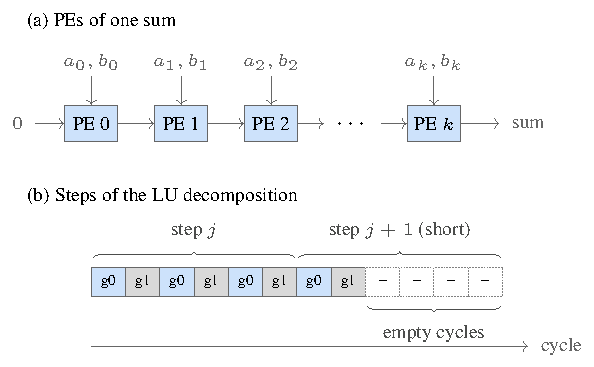
\includegraphics{Images/FLUXO/hw_c4.pdf}
\end{minipage}
\vspace{4pt}
\legend{Source: the author. g0, g1: groups of matrices of the batch, one per cycle; there are 16 groups for the 151-cycle limit and 8 for the 113-cycle limit.}
\end{figure}

% ---------------------------------------------------------------------
\subsection{\texorpdfstring{Test matrices}{Test matrices}}\label{subsec:hw-matrizes}
% ---------------------------------------------------------------------
The hardware was tested with the same $\mathbf{G}_c$ matrices that BCD-MMSE inverts in the SER curves, with 1 iteration. These matrices were saved before inversion, in each of the 5 distinct test conditions (Section~\ref{subsec:setup_condicoes}). In each condition, a sample was saved: some matrices randomly selected by configuration and SNR point, and the most extreme in range and precision, such as those with the largest element and the largest condition number. QPSK configurations were excluded because the modulation does not change $\mathbf{G}_c$.

The testbench inverts 20 matrices randomly selected from this sample. In the $16 \times 16$ circuit, these matrices come only from configurations 1A--1H. In architectures with batch, the 20 matrices are repeated until at least 3 batches are completed.


% FONTE: rodar_potencia.py (sinteses/*_vivado/potencia/): 20 matrizes sorteadas com
%   semente fixa; 16x16: 1A, 1B, 1E e 1F; 32x32: 2A, 2B, 2E e 2F; grupo 3 fora da potência
%   (decisão da autora). tb_potencia.cpp da 606 (linhas 57-71: lotes = max(3, ceil(20/LOTE)));
%   potencia.csv: 36 (606), 48 (455), 96 (152 e 114), 20 nas outras.

% ---------------------------------------------------------------------
\subsection{\texorpdfstring{Power and energy}{Power and energy}}\label{subsec:hw-potencia}
% ---------------------------------------------------------------------
Power was estimated from the switching activity of the routed design: the version without optimizations under the 5 test conditions, and each optimized architecture only under its own. Vivado generates a functional netlist, which is simulated with the testbench. The simulation checks the inverses byte by byte against the C code and records how many times each signal changes value in a SAIF (Switching Activity Interchange Format) file. Vivado then reads this file and reports the power.

Energy per inversion is defined as the dynamic power multiplied by the average time required for an inversion. This duration is calculated as the interval between two inversions, measured during the netlist simulation, multiplied by the 10~ns clock period. In architectures that employ batch processing, the interval between two batches is divided by $n$.
\textcolor{red}{A potência estática é a potência total menos a dinâmica.}
% Retirado em 2026-11-13 (a figura potencia_media_condicao saiu dos Resultados em 2026-11-09):
%   A potência média no ritmo exigido de cada condição de teste soma a potência estática e a
%   energia de 275 inversões dividida por T_c. Ela supõe que, depois de inverter as 275 matrizes
%   do bloco, o módulo fica parado até o próximo bloco e só gasta a potência estática.
% FONTE: memória tcc-pacote-servidor-2023 (convenção da energia). Intervalo tirado do
%   xsim_<cenário>.log do servidor, não do ciclos_medios do potencia.csv, que inclui o
%   enchimento do pipeline do primeiro lote.


% =====================================================================
% \section{\texorpdfstring{Organization of the results}{Organization of the % results}}\label{sec:organizacao-resultados}
% =====================================================================


% ---------------------------------------------------------------------
% 1.6  ORGANIZAÇÃO DOS RESULTADOS                 -> fim da Metodologia
% ---------------------------------------------------------------------
% The results are grouped according to the physical characteristics of the base station: the size of the inversion circuit ($16 \times 16$ or $32 \times 32$), the number of antennas $M$, and the number of clusters $C$. Within each group, the modulation, $K$, and IoTh vary. Thus, there are three groups: configurations 1A–1H ($M = 128$, $C = 8$, $16 \times 16$ circuit), 2A–2H ($M = 256$, $C = 8$, $32 \times 32$ circuit), and 3A–3H ($M = 256$, $C = 16$, $16 \times 16$ circuit). \textcolor{red}{Os mapas de aumento de SNR, as curvas, as barras e os perfis de mobilidade são apresentados por grupo (Seção~\ref{sec:resultados-formato}). Os resultados de hardware, de vazão e de atraso são apresentados por condição de teste (Seção~\ref{sec:resultados-hardware}).}


% =====================================================================
\chapter{Resultados}
% =====================================================================

% =====================================================================
% RASCUNHO -- seção "Setup de simulação" reorganizada por módulo do simulador
% ---------------------------------------------------------------------
% Incluído em 9-results.tex por \input{chapters/rascunho_setup_simulacao}.
% Substitui o setup antigo (cópia em rascunho_setup_antigo.tex) e
% rascunho_setup_tabelas.tex (as tabelas estão copiadas aqui).
% A entrada tomasin-interference precisa ir para o biblio.bib.
%
% Marcas:
%   % AUTORA (9-results.tex:NNN)  -> texto seu, sem alteração, só mudou de lugar
%   % NOVO                        -> texto proposto; cada frase tem FONTE ou SEM FONTE
%
% Chaves de citação: zhao2025jsac (já existe); tomasin-interference (em
% constraints/rascunho_referencias.bib). ATENÇÃO: rascunho_bloco_canal.tex
% usa a chave antiga zhao-lmmse; trocar por zhao2025jsac se for aproveitado.
% "Lnnn" = linha do paper.md do artigo base.
% =====================================================================

\section{Simulation setup}
The simulation parameters are organized as the simulation flow of Figure~\ref{fig:fluxo_simulacao}. The base station configurations are inputs of both parts of the flow. The channels are generated before the simulation, by a MATLAB script that runs QuaDRiGa (Section~\ref{subsec:setup_canal}). The Python simulator reads the stored channels and sets the other parameters: test conditions, signal and noise, receiver and evaluation (Section~\ref{subsec:setup_python}). In the tables, the source column gives the reference of each value, and the name in the code gives the variable that sets it. \textcolor{red}{The parameter tables are in Appendix~\ref{ap:parametros}.}



% TOM: Zhao et al. é a referência do modelo, não objeto de reprodução.


% Subseção "Base Stations Configurations" (texto e Tabela tab:paineis) movida para
%   METODOLOGIA/configuracoes.tex em 2026-11-04, para os nomes 1A-3D serem definidos
%   antes de serem usados na Metodologia.

% ---------------------------------------------------------------------
\subsection{Channel Generation in QuaDRiGa}\label{subsec:setup_canal}
% ---------------------------------------------------------------------

Table~\ref{tab:param_canal} shows the parameters of the MATLAB script that generates the channel matrices $\mathbf{H}$ and $\overline{\mathbf{H}}$. The remaining QuaDRiGa parameters were kept at their default values \cite{quadriga-manual}.

The BS features a uniform linear array (ULA) of $M$ antennas, with a standard spacing of half a wavelength ($\lambda/2$) of the operating signal. The antennas at both the BS and the UEs are omnidirectional, meaning they provide the same gain in all directions.

For each realization, the script randomly determines the positions of the $K$ target UEs and the $r$ interferers. The distance is sampled such that the UE density remains uniform across the entire area. The random seed used for this sampling is always the realization number. Based on these positions, QuaDRiGa generates the frequency-domain channel response between each BS antenna and each UE within the propagation scenario.





In this work, the \texttt{3GPP\_\allowbreak{}38.901\_\allowbreak{}UMa\_\allowbreak{}NLOS} propagation scenario was used, which represents an urban macrocell (UMa) with no line-of-sight (NLoS) between the base station (BS) and the user equipment (UEs). Table~\ref{tab:cenario_uma} presents the valid range for the UMa propagation scenario and the values selected. The system model assumes a flat-fading channel, in which all subcarriers within a physical resource block (PRB) experience the same channel conditions.








% ---------------------------------------------------------------------
\subsection{Python Simulator}\label{subsec:setup_python}
% ---------------------------------------------------------------------

The Python simulator reads the stored channels and runs the rest of the simulation flow. Its parameters are grouped as in Figure~\textcolor{red}{\ref{fig:fluxo_python}}: test conditions, signal and noise, receiver and evaluation. \textcolor{red}{The test conditions are described in Section~\ref{subsec:setup_condicoes}.}

% MOVIDO (2026-11-04): a subsubseção "Test Conditions" (texto da autora e Tabela
%   tab:condicoes_teste) foi para METODOLOGIA/condicoes-teste.tex, junto com a escolha do N.


% ---------------------------------------------------------------------
\subsubsection{Signal and Noise}\label{subsec:setup_ruido}
% ---------------------------------------------------------------------

% NOVO
Table~\ref{tab:param_ruido} shows the parameters used to read the channels and to generate the transmitted symbols and the noise.


The SNR depends solely on the ratio between the symbol energy $E_s$ and the thermal noise power $\sigma^2$, as defined by the parameter \texttt{M5\_\allowbreak{}Noise.\allowbreak{}snr\_\allowbreak{}definition}. Accordingly, the constellations were normalized to have unit average energy (parameter \texttt{M4\_\allowbreak{}Source.\allowbreak{}unit\_\allowbreak{}energy\_\allowbreak{}constellation}), and the symbol energy was set to $E_s = 1$ (parameter \texttt{M4\_\allowbreak{}Source.\allowbreak{}Es}). Thus, the power $\sigma^2$ could be calculated based on the SNR to be simulated.

Furthermore, the power of the UEs was adjusted via channel normalization, defined by the parameter \texttt{M2\_\allowbreak{}Channel.\allowbreak{}normalization}, ensuring that signals from UEs located at varying distances arrived at the BS with the same average power.

With the channel normalized, each of the $r$ interferers reaches every BS antenna with the same average power. In this scenario, the interference received at each antenna is scaled by the number of interferers, $r$. To ensure that the ratio of interference to thermal noise at each antenna equals the IoTh value specified in the configuration (parameter \texttt{M5\_\allowbreak{}Noise.\allowbreak{}iot\_\allowbreak{}db}), the power $\beta$ of each interferer is divided by $r$. This convention is governed by the parameter \texttt{M5\_\allowbreak{}Noise.\allowbreak{}beta\_\allowbreak{}convention} and follows the approach of averaging interference at each antenna, a method also employed in \cite{tomasin-interference}.

The parameter \texttt{M5\_\allowbreak{}Noise.\allowbreak{}data\_\allowbreak{}noise\_\allowbreak{}independent} specifies that the noise affecting the data symbols is drawn independently from the $N$ noise samples used to estimate the covariance matrix $\hat{\mathbf{R}}$. The parameter \texttt{M5\_\allowbreak{}Noise.\allowbreak{}resample\_\allowbreak{}noise\_\allowbreak{}per\_\allowbreak{}realization} specifies that the $N$ samples are re-drawn for each channel realization and each SNR point. This mimics the real behavior of the system, where samples come from the pilot REs and the data occupies other REs.

\subsubsection{Receiver}\label{subsec:setup_receptor}
% ---------------------------------------------------------------------

Table~\ref{tab:param_receptor} shows the parameters for antenna partitioning, covariance estimation, and the equalizers.

% FONTES: M_c = M/C L577, L85; N L577, L640; covariância eq. (6) L119 e L125;
%   H perfeito L63 e nota 2 (L817); equalizadores L581 e Figura 8;
%   iterações e posto L587, L591; Gauss-Seidel L398, nota 6 (L450);
%   L = K L150, L184, L593; W reaproveitado L61, L561; ZF citado em L581 sem fórmula.
% CORREÇÃO em relação à tabela antiga: W e as amostras de ruído são refeitos a
%   cada ponto de SNR, não só a cada realização (m1_driver.run_panel).
% LEMBRETE: o Ledoit-Wolf também é aplicado no R_cc do BCD (m7_equalizers.bcd_mmse).
%   Com N = 192 o bloco M_c x M_c tem inversa; com N = 12 (HST) não tem, pois
%   N < M_c. O módulo alvo do constraints.csv inverte o R_cc sem ajuste.
% N e portadora por condição: params.M1_Driver.test_conditions; run_figure8.py --conditions.


Each cluster is assigned neighboring antennas (parameter \texttt{M3\_\allowbreak{}Clustering.\allowbreak{}mapping}). The first cluster is assigned antennas 1 to $M_c$, the second is assigned antennas $M_c+1$ to $2M_c$, and so on. All clusters have the same number of antennas (parameter \texttt{M3\_\allowbreak{}Clustering.\allowbreak{}equal\_\allowbreak{}cluster\_\allowbreak{}size}).

The equalizers receive the true $\mathbf{H}$ channel, without channel estimation (parameter \texttt{M7\_\allowbreak{}Equalizers.\allowbreak{}perfect\_\allowbreak{}csi}), as in \cite{zhao2025jsac}. The BCD-MMSE was simulated with 1 iteration (parameter \texttt{M7\_\allowbreak{}Equalizers.\allowbreak{}bcd\_\allowbreak{}iterations}). The DUs update sequentially, from $c = 1$ to $C$, and each one uses the result of the previous one (parameter \texttt{M7\_\allowbreak{}Equalizers.\allowbreak{}bcd\_\allowbreak{}update\_\allowbreak{}rule}) \cite{zhao2025jsac}.

% FONTE: L63, nota 2 (L817).

% FONTE: paper.md:590-591 (Fig. 8 com 1 iteração); Gauss-Seidel L398, nota 6 (L450).
% DECISÃO da autora (2026-11-04): a primeira versão usa só 1 iteração. As rodadas [1], [4]
%   e [5] também têm 4 iterações (mapas iter4); podem entrar depois, se houver tempo.
%   Nesse caso, este parágrafo vira "1 e 4 iterações".





% ---------------------------------------------------------------------
\subsubsection{Evaluation}\label{subsec:setup_avaliacao}
% ---------------------------------------------------------------------


Table~\ref{tab:param_avaliacao} shows how the results are measured.
The random number generator seed was set to 0, so that the results can be replicated.




% =====================================================================
% =====================================================================
\section{\texorpdfstring{Selection and analysis of word format}{Selection of word format}}\label{sec:resultados-formato}

This section presents the results of the validation of the 10 formats (Section~\ref{subsec:validacao}). The results are grouped by the number of the configuration, which sets $M$, $C$ and the size of the inversion circuit (Section~\ref{subsec:configuracoes-bs}): group 1 ($M = 128$, $C = 8$, $16 \times 16$ circuit), group 2 ($M = 256$, $C = 8$, $32 \times 32$ circuit) and group 3 ($M = 256$, $C = 16$, $16 \times 16$ circuit). All configurations of a group use the same circuit, and only the modulation, $K$ and IoTh change between them.

For each group, the section presents the effect of the format on the SNR increase, the chosen formats, and how much of the increase over LMMSE comes from decentralization and how much from the format. Then, Section~\ref{subsec:perfis-mobilidade} shows whether the choice of format changes with the mobility profile. \textcolor{red}{Depois, a Seção~\ref{sec:resultados-curvas} mostra as curvas de SER dos três grupos.} The hardware, throughput and delay results are presented by test condition, because each condition has its own architecture, set by its cycle limit (Section~\ref{sec:resultados-hardware}).

% ---------------------------------------------------------------------
\subsection{\texorpdfstring{\textcolor{red}{Grupo 1: $M = 128$, $C = 8$}}{Grupo 1: M = 128, C = 8}}\label{subsec:resultados-grupo1}\label{subsec:mapas-perda}
% ---------------------------------------------------------------------


\begin{figure}[!htb]
\caption{\textcolor{red}{Maior aumento de SNR, em dB, no grupo 1, configurações 1A a 1H ($M = 128$, $C = 8$, $M_c = 16$).}}
\label{fig:mapa-grupo1}
\vspace{4pt} % a classe zera o espaço entre a caption e a figura
\centering
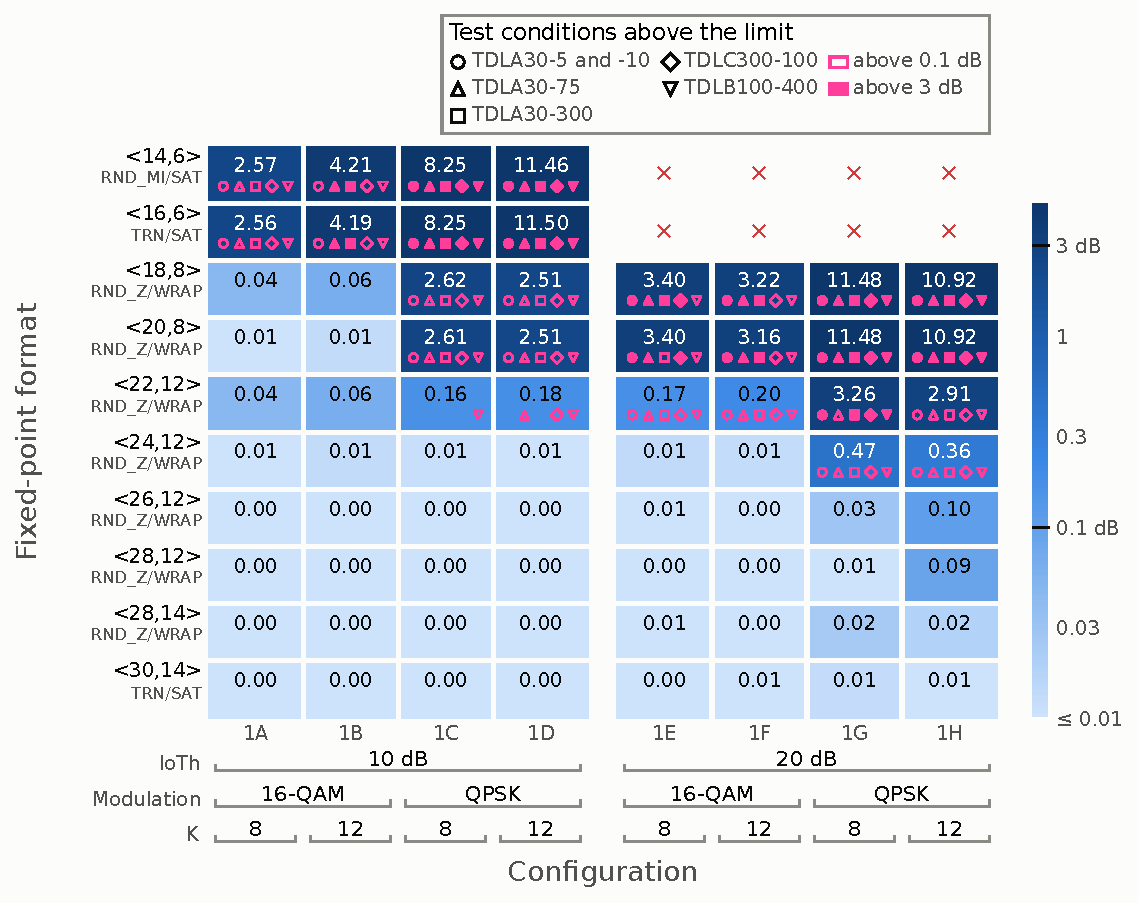
\includegraphics[width=\textwidth]{Images/RESULTADOS/mapa_snr_grupo1.pdf}
\vspace{4pt}
\legend{\textcolor{red}{Fonte: a autora. Abaixo do formato, o modo de quantização e o de estouro, sem o prefixo AP\_.}}
\end{figure}

Figure~\ref{fig:mapa-grupo1} shows, on a logarithmic color scale, the largest SNR increase of each format (rows) in each configuration (columns), among the 5 simulated test conditions (Section~\ref{subsec:setup_condicoes}). Below the value, unfilled symbols mark the test conditions above 0.1~dB, and filled symbols, those above 3~dB. The circle stands for TDLA30-5 and TDLA30-10, which share the same SER curves. A $\times$ marks a cell where some test condition does not reach $\mathrm{SER} = 10^{-2}$. The maps of groups 2 and 3 follow the same layout.

For each threshold, the chosen format is the smallest one in which all configurations stay within it (Section~\ref{sec:formato}): $\langle 24,12\rangle$ for 3~dB and $\langle 26,12\rangle$ for 0.1~dB. The QPSK configurations with IoTh of 20~dB (1G and 1H) set both formats. When only the configurations with IoTh of 10~dB (1A to 1D) are considered, the chosen formats are $\langle 18,8\rangle$ and $\langle 24,12\rangle$, respectively.


% -----------------------

\label{sec:resultados-descentralizacao}\label{subsec:descentralizacao}%

\begin{figure}[!htb]
\caption{\textcolor{red}{Aumento de SNR do BCD-MMSE sobre o LMMSE no grupo 1 ($M = 128$, $C = 8$, $M_c = 16$), no pior caso de cada barra.}}
\label{fig:descentralizacao-grupo1}
\vspace{4pt} % a classe zera o espaço entre a caption e a figura
\centering
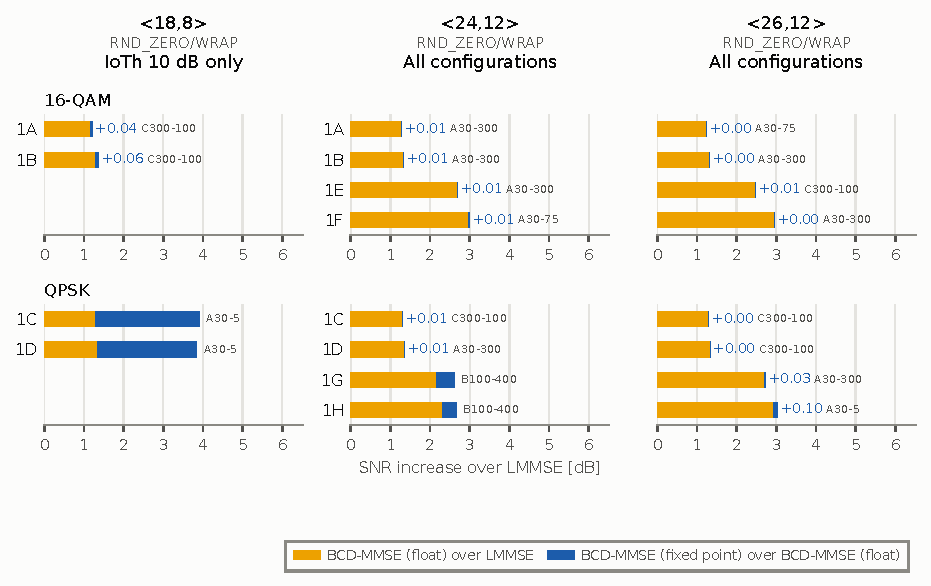
\includegraphics[width=\textwidth]{Images/RESULTADOS/descentralizacao_grupo1.pdf}
\vspace{4pt}
\legend{\textcolor{red}{Fonte: a autora.}}
\end{figure}

Figure~\ref{fig:descentralizacao-grupo1} illustrates the source of the SNR gain provided by BCD-MMSE over LMMSE at an $\mathrm{SER}$ of $10^{-2}$. The yellow bar represents the gain resulting from decentralization, that is, the difference between LMMSE and floating-point BCD-MMSE. The blue bar represents the gain (or impact) attributed to the numerical format, that is, the difference between floating-point and fixed-point BCD-MMSE, with the specific value indicated at the end of the bar. Each plot corresponds to a chosen format from the group (Table~\ref{tab:formatos-escolhidos}), and each bar represents a specific configuration. For each configuration, the test condition under which the format yields the greatest SNR increase was selected, and the name of this condition is labeled next to the bar.

In Group 1, decentralization provides the largest SNR gain when the IoTh is 20~dB. With 16-QAM, the gain attributed to the numerical format is negligible. In contrast, with QPSK, this gain is significantly larger, reaching 2.6~dB for the $\langle 18,8\rangle$ format, which exceeds the gain provided by decentralization. Thus, QPSK appears to be more sensitive to the approximations introduced by the numerical format than 16-QAM.

% -----------------------

\FloatBarrier
% ---------------------------------------------------------------------
\subsection{\texorpdfstring{\textcolor{red}{Grupo 2: $M = 256$, $C = 8$}}{Grupo 2: M = 256, C = 8}}\label{subsec:resultados-grupo2}\label{subsubsec:mapa-grupo2}
% ---------------------------------------------------------------------

\begin{figure}[!htb]
\caption{\textcolor{red}{Maior aumento de SNR, em dB, no grupo 2, configurações 2A a 2H ($M = 256$, $C = 8$, $M_c = 32$).}}
\label{fig:mapa-grupo2}
\vspace{4pt} % a classe zera o espaço entre a caption e a figura
\centering
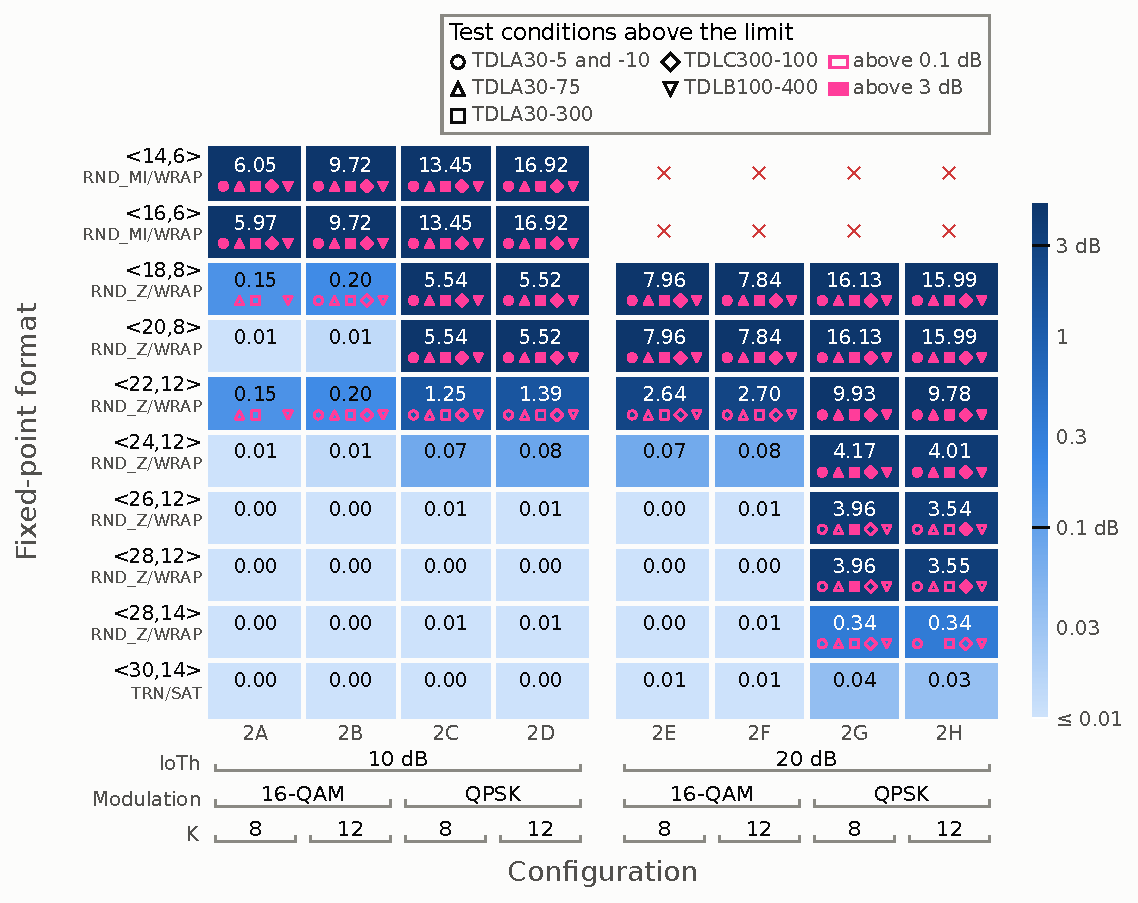
\includegraphics[width=\textwidth]{Images/RESULTADOS/mapa_snr_grupo2.pdf}
\vspace{4pt}
\legend{\textcolor{red}{Fonte: a autora. Abaixo do formato, o modo de quantização e o de estouro, sem o prefixo AP\_.}}
\end{figure}

\begin{figure}[!htb]
\caption{\textcolor{red}{Aumento de SNR do BCD-MMSE sobre o LMMSE no grupo 2 ($M = 256$, $C = 8$, $M_c = 32$), no pior caso de cada barra.}}
\label{fig:descentralizacao-grupo2}
\vspace{4pt} % a classe zera o espaço entre a caption e a figura
\centering
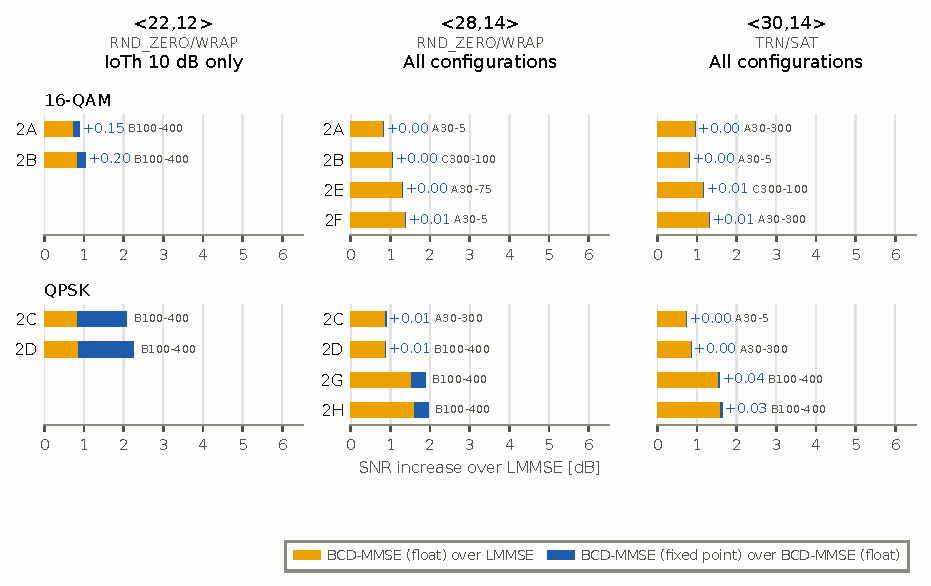
\includegraphics[width=\textwidth]{Images/RESULTADOS/descentralizacao_grupo2.pdf}
\vspace{4pt}
\legend{\textcolor{red}{Fonte: a autora.}}
\end{figure}

Group 2 has twice as many antennas as group 1, with the same number of clusters. Thus, each cluster has 32 antennas, not 16. In the map (Figure \ref{fig:mapa-grupo2}), the greatest increase in SNR in the smaller formats is greater than in group 1. Furthermore, the increase remains above 3 dB even in larger formats. In 2G and 2H, this goes up to $\langle 28,12\rangle$, while 1G and 1H remain below 3 dB from $\langle 24,12\rangle$. Therefore, the chosen formats are larger: $\langle 28,14\rangle$ at the 3 dB limit and $\langle 30,14\rangle$ at the 0.1 dB limit. As in group 1, the two are defined by 2G and 2H, with QPSK and IoTh of 20~dB.

In 2G and 2H, from $\langle 24,12\rangle$ to $\langle 28,12\rangle$, the increase hardly changes. These formats only gain fractional bits. The increase only decreases at $\langle 28,14\rangle$, which has 2 more integer bits. Therefore, group 2 needs more integer bits than group 1. A likely explanation is the SNR at which the group operates. With more antennas, the equalizers need less SNR, as also happens in \cite{zhao2025jsac}. In the simulation, the symbol energy $E_s$ is fixed, and the SNR varies according to the thermal noise power, $\sigma^2$ (Equation~\ref{eq:snr}). With a fixed IoTh, the interference scales with $\sigma^2$ (Equation~\ref{eq:iot}). Consequently, as the SNR decreases, the combined noise and interference become stronger, causing $\hat{\mathbf R}_{cc}$ to increase as well. Since $\mathbf G_c$ is formed by adding $\hat{\mathbf R}_{cc}$ to the channel term (Section~\ref{subsec:bcd}), the elements of $\mathbf G_c$ also increase. At the same SNR, an IoTh of 20 dB results in ten times more noise-plus-interference than an IoTh of 10 dB, leading to even larger values for these elements.
In Figure \ref{fig:descentralizacao-grupo2}, decentralization increases the SNR less than in group 1. That is, with more antennas, the BCD-MMSE gets closer to the LMMSE, as also happens in \cite{zhao2025jsac}. The increase in format size is also smaller because the chosen formats are larger. However, as in group 1, it is larger with QPSK than with 16-QAM.


% ---------------------------------------------------------------------
\subsection{\texorpdfstring{\textcolor{red}{Grupo 3: $M = 256$, $C = 16$}}{Grupo 3: M = 256, C = 16}}\label{subsec:resultados-grupo3}\label{subsubsec:mapa-grupo3}
% ---------------------------------------------------------------------

\begin{figure}[!htb]
\caption{\textcolor{red}{Maior aumento de SNR, em dB, no grupo 3, configurações 3A a 3H ($M = 256$, $C = 16$, $M_c = 16$).}}
\label{fig:mapa-grupo3}
\vspace{4pt} % a classe zera o espaço entre a caption e a figura
\centering
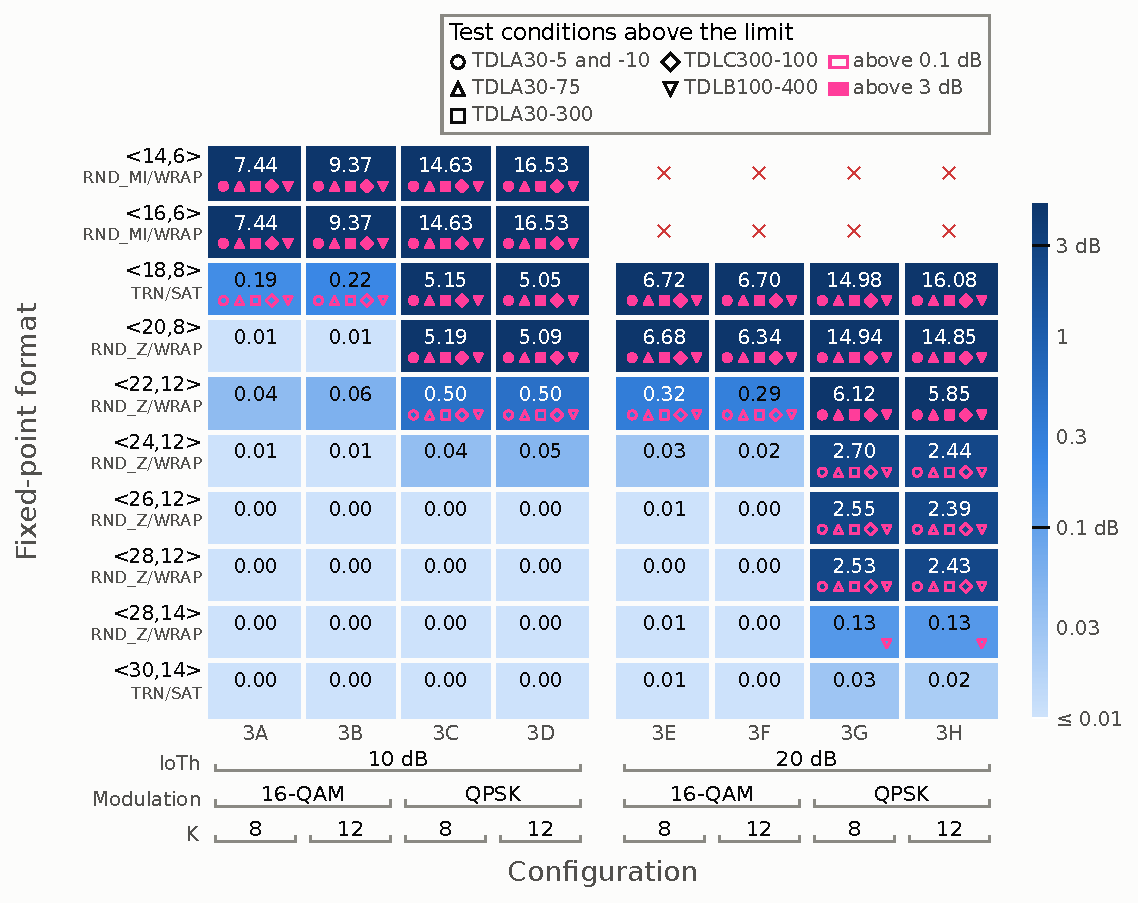
\includegraphics[width=\textwidth]{Images/RESULTADOS/mapa_snr_grupo3.pdf}
\vspace{4pt}
\legend{\textcolor{red}{Fonte: a autora. Abaixo do formato, o modo de quantização e o de estouro, sem o prefixo AP\_.}}
\end{figure}

\begin{figure}[!htb]
\caption{\textcolor{red}{Aumento de SNR do BCD-MMSE sobre o LMMSE no grupo 3 ($M = 256$, $C = 16$, $M_c = 16$), no pior caso de cada barra.}}
\label{fig:descentralizacao-grupo3}
\vspace{4pt} % a classe zera o espaço entre a caption e a figura
\centering
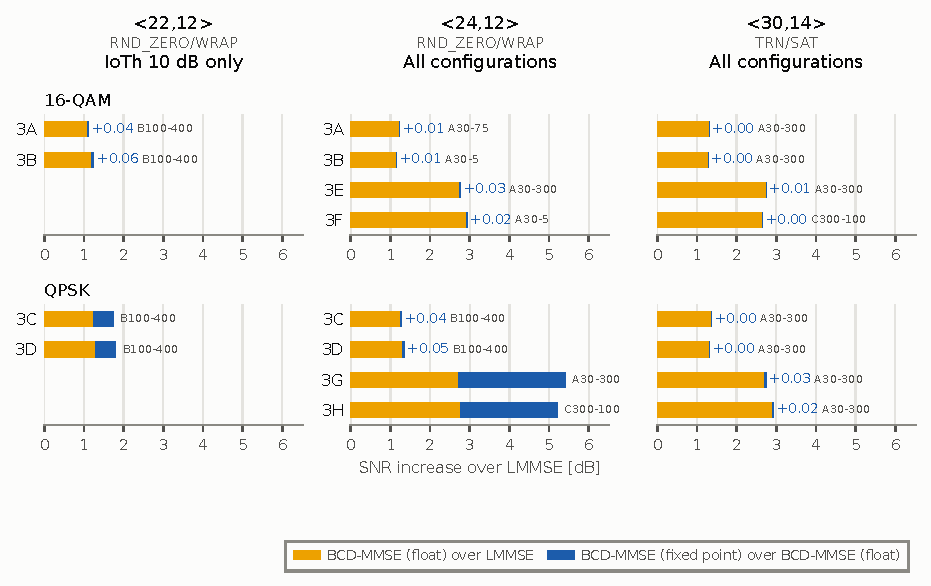
\includegraphics[width=\textwidth]{Images/RESULTADOS/descentralizacao_grupo3.pdf}
\vspace{4pt}
\legend{\textcolor{red}{Fonte: a autora.}}
\end{figure}


Group 3 has the same number of antennas as Group 2, but twice the number of clusters. Consequently, each cluster contains 16 antennas, just as in Group 1. As shown in the map (Figure~\ref{fig:mapa-grupo3}), the most significant gain for smaller formats occurs near Group 2. However, at the 3~dB threshold, the format is $\langle 24,12\rangle$, the same as in Group 1 and smaller than the $\langle 28,14\rangle$ format found in Group 2. This suggests that, in addition to the total number of antennas, the cluster size also influences the format.


For the $\langle 24,12\rangle$ format, 3G and 3H lie close to the 3~dB threshold. In subsequent formats, similar to what is observed in Group 2, the gain for these cases remains nearly constant up to $\langle 28,12\rangle$, only decreasing when two additional bits are introduced in the $\langle 28,14\rangle$ format. Even then, it remains above 0.1~dB. Therefore, at the 0.1~dB threshold, the format is $\langle 30,14\rangle$, which is the same as in Group 2.

\label{subsubsec:descentralizacao-grupo3}%

In Figure~\ref{fig:descentralizacao-grupo3}, decentralization yields a greater increase in SNR compared to Group 2, bringing it closer to the levels seen in Group 1. Since the clusters contain fewer antennas, each one utilizes a smaller block of the covariance matrix. With a higher number of clusters, the BCD-MMSE performance deviates further from the LMMSE, a phenomenon also noted in \cite{zhao2025jsac}. Using QPSK, for the $\langle 24,12\rangle$ format, the gain provided by the format for 3G and 3H is nearly equivalent to the gain achieved through decentralization. For $\langle 22,12\rangle$, with an IoTh of only 10~dB, the gap is smaller than in group 2.


Thus, across the three groups, the primary factor driving the divergence between BCD-MMSE and LMMSE depends on the modulation scheme. With 16-QAM, the impact of the numerical format is almost negligible, and the decentralization effect carries more weight. With QPSK, for the formats at the 3~dB threshold, the numerical format carries as much weight as the decentralization, or even more; this is the case for $\langle 18,8\rangle$ in group 1, $\langle 22,12\rangle$ in group 2, and $\langle 24,12\rangle$ in group 3. For the formats at the 0.1~dB threshold, the decentralization effect is the dominant factor in all cases.

\FloatBarrier
% ---------------------------------------------------------------------
\subsection{\texorpdfstring{\textcolor{red}{Formatos escolhidos}}{Formatos escolhidos}}\label{subsec:formatos-escolhidos}
% ---------------------------------------------------------------------
\begin{table}[htbp]
\caption{\textcolor{red}{Formatos escolhidos em cada grupo de configurações.}}
\label{tab:formatos-escolhidos}
\vspace{4pt} % a classe zera o espaço entre a caption e a tabela
\centering
\footnotesize
\renewcommand{\arraystretch}{1.2}
\setlength{\tabcolsep}{3pt}
\begin{tabular}{>{\raggedright\arraybackslash}p{2.4cm}ccc}
\toprule
\textbf{Criterion} & \textbf{Group 1} & \textbf{Group 2} & \textbf{Group 3} \\
\midrule
\multicolumn{4}{l}{\textbf{All configurations (A to H)}} \\
Increase up to 3~dB & \begin{tabular}[c]{@{}c@{}}$\langle 24,12\rangle$\\ \texttt{AP\_RND\_ZERO}/\texttt{AP\_WRAP}\end{tabular} & \begin{tabular}[c]{@{}c@{}}$\langle 28,14\rangle$\\ \texttt{AP\_RND\_ZERO}/\texttt{AP\_WRAP}\end{tabular} & \begin{tabular}[c]{@{}c@{}}$\langle 24,12\rangle$\\ \texttt{AP\_RND\_ZERO}/\texttt{AP\_WRAP}\end{tabular} \\
\addlinespace
Increase up to 0.1~dB & \begin{tabular}[c]{@{}c@{}}$\langle 26,12\rangle$\\ \texttt{AP\_RND\_ZERO}/\texttt{AP\_WRAP}\end{tabular} & \begin{tabular}[c]{@{}c@{}}$\langle 30,14\rangle$\\ \texttt{AP\_TRN}/\texttt{AP\_SAT}\end{tabular} & \begin{tabular}[c]{@{}c@{}}$\langle 30,14\rangle$\\ \texttt{AP\_TRN}/\texttt{AP\_SAT}\end{tabular} \\
\midrule
\multicolumn{4}{l}{\textbf{IoTh of 10~dB (A to D)}} \\
Increase up to 3~dB & \begin{tabular}[c]{@{}c@{}}$\langle 18,8\rangle$\\ \texttt{AP\_RND\_ZERO}/\texttt{AP\_WRAP}\end{tabular} & \begin{tabular}[c]{@{}c@{}}$\langle 22,12\rangle$\\ \texttt{AP\_RND\_ZERO}/\texttt{AP\_WRAP}\end{tabular} & \begin{tabular}[c]{@{}c@{}}$\langle 22,12\rangle$\\ \texttt{AP\_RND\_ZERO}/\texttt{AP\_WRAP}\end{tabular} \\
\addlinespace
Increase up to 0.1~dB & \begin{tabular}[c]{@{}c@{}}$\langle 24,12\rangle$\\ \texttt{AP\_RND\_ZERO}/\texttt{AP\_WRAP}\end{tabular} & \begin{tabular}[c]{@{}c@{}}$\langle 24,12\rangle$\\ \texttt{AP\_RND\_ZERO}/\texttt{AP\_WRAP}\end{tabular} & \begin{tabular}[c]{@{}c@{}}$\langle 24,12\rangle$\\ \texttt{AP\_RND\_ZERO}/\texttt{AP\_WRAP}\end{tabular} \\
\bottomrule
\end{tabular}
\vspace{4pt}
\legend{\textcolor{red}{Fonte: a autora. Abaixo do formato, o modo de quantização e o de estouro.}}
\end{table}

Table~\ref{tab:formatos-escolhidos} presents the formats selected across the three groups, both with all configurations and with only the 10~dB IoTh configurations (A through D). Excluding the 20~dB IoTh configurations results in formats that are 2 to 6 bits smaller, with the 0.1~dB format becoming $\langle 24,12\rangle$ in all three groups. Since some formats overlap, there are three distinct formats to synthesize for groups 1 and 3, and four for group 2 (Section~\ref{sec:resultados-hardware}).


\FloatBarrier
% =====================================================================
\section{\texorpdfstring{Mobility profiles}{Mobility profiles}}\label{subsec:perfis-mobilidade}
% =====================================================================
Figure~\ref{fig:perfis-formatos} shows the largest SNR increase of each of the 10 validated formats (Section~\ref{subsec:validacao}) for each mobility profile (Section~\ref{subsec:setup_condicoes}). Each row represents a group. The first column includes all configurations, while the second column is restricted to those with an IoTh of 10~dB. Each data point represents the largest increase among the configurations within that column under the conditions of the respective profile. The triangle on the right-hand side marks the first format, from top to bottom, that falls within each limit; this is the format selected for that profile.

For most formats, the data points for both profiles are close to one another, with the high-mobility point appearing either to the right of or directly atop the low-mobility point. In other words, the mobility profile has little impact on the SNR increase. However, under low-mobility conditions alone, the selected format would be 2 bits smaller in two instances: $\langle 26,12\rangle$ instead of $\langle 28,14\rangle$ in group 2, with the 3~dB limit, and $\langle 28,14\rangle$ instead of $\langle 30,14\rangle$ in group 3, with the 0.1~dB limit. In all other cases, both profiles select the same format. Consequently, the high-mobility profile determines the format. Appendix~\ref{ap:perfis-configuracao} presents the SNR increase of each configuration with the selected formats.

\begin{figure}[!htb]
\caption{\textcolor{red}{Largest SNR increase, in dB, of each format in each mobility profile, in the three groups.}}
\label{fig:perfis-formatos}
\vspace{4pt} % a classe zera o espaço entre a caption e a figura
\centering
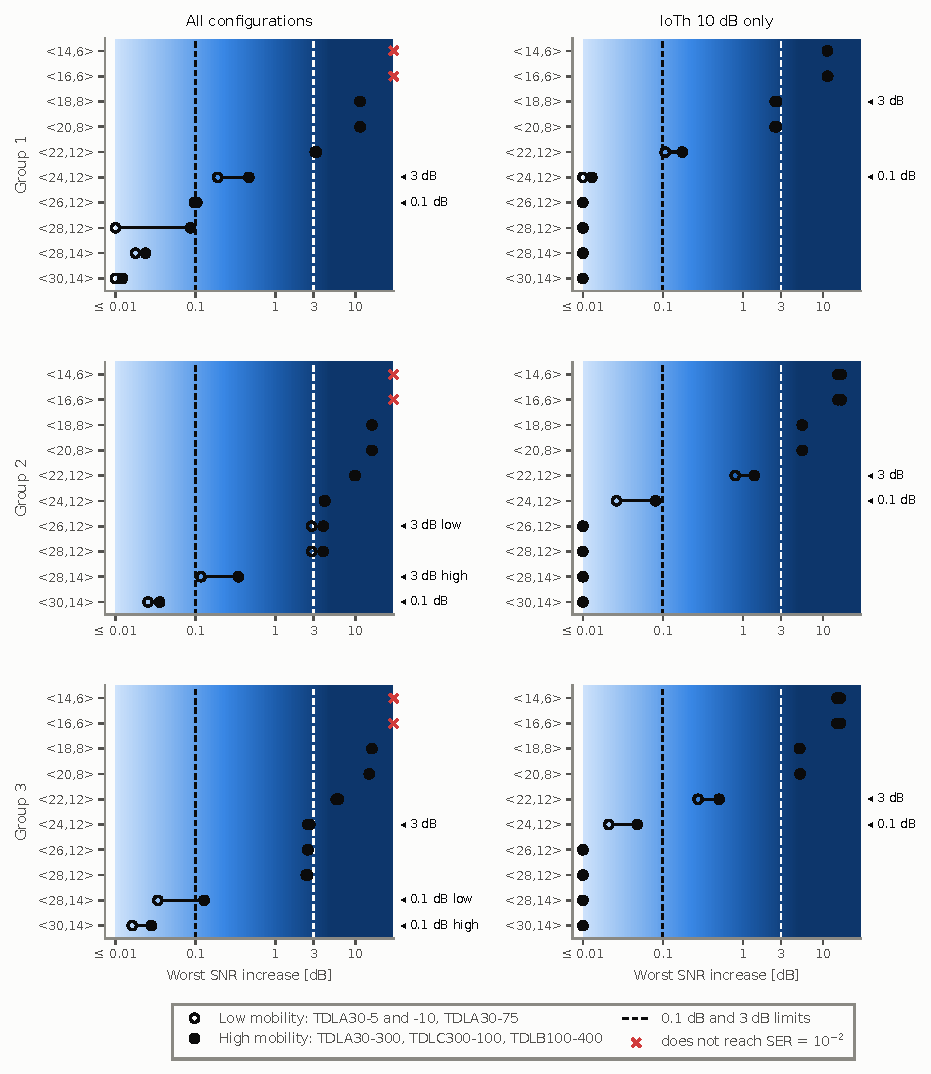
\includegraphics[width=\textwidth]{Images/RESULTADOS/perfis_mobilidade_formatos.pdf}
\vspace{4pt}
\legend{\textcolor{red}{Source: the author. Each format uses the same mode as in the SNR increase maps (Figures~\ref{fig:mapa-grupo1} to \ref{fig:mapa-grupo3}): RND\_ZERO/WRAP, except $\langle 14,6\rangle$ in RND\_MIN\_INF/SAT in group 1 and RND\_MIN\_INF/WRAP in groups 2 and 3; $\langle 16,6\rangle$ in TRN/SAT in group 1 and RND\_MIN\_INF/WRAP in groups 2 and 3; $\langle 18,8\rangle$ in TRN/SAT in group 3; and $\langle 30,14\rangle$ in TRN/SAT in all three groups.}}
\end{figure}


\FloatBarrier
% =====================================================================
\section{\texorpdfstring{SER curves}{SER curves}}\label{sec:resultados-curvas}\label{subsec:curvas-ser}
% =====================================================================

Figure~\ref{fig:curvas-ser-grupos} shows the SER curves for LMMSE and ZF (in floating-point) and BCD-MMSE (in fixed-point) for the TDLC300-100 channel model. The analysis here is not limited to the $\mathrm{SER} = 10^{-2}$ point; the curves cover the entire SNR range, from $-20$ to 10~dB. Each row of plots represents a group of configurations, while each column corresponds to a criterion from Table~\ref{tab:formatos-escolhidos}; the BCD-MMSE in each plot utilizes the format selected for that specific case. The first two columns include all configurations, the first with the 3~dB format and the second with the 0.1~dB format. The third column contains only the configurations with an IoTh of 10~dB, using the 3~dB format selected for them. The ZF performance remains unchanged by the format and is included in the plots as a worst-case reference; for the sake of clarity, it is omitted from the third column. The curves for the remaining test conditions can be found in Appendix~\ref{ap:curvas-ser}.

\begin{figure}[!htb]
\caption{\textcolor{red}{Curvas de SER dos três grupos na TDLC300-100, nos formatos escolhidos.}}
\label{fig:curvas-ser-grupos}
\vspace{4pt} % a classe zera o espaço entre a caption e a figura
\centering
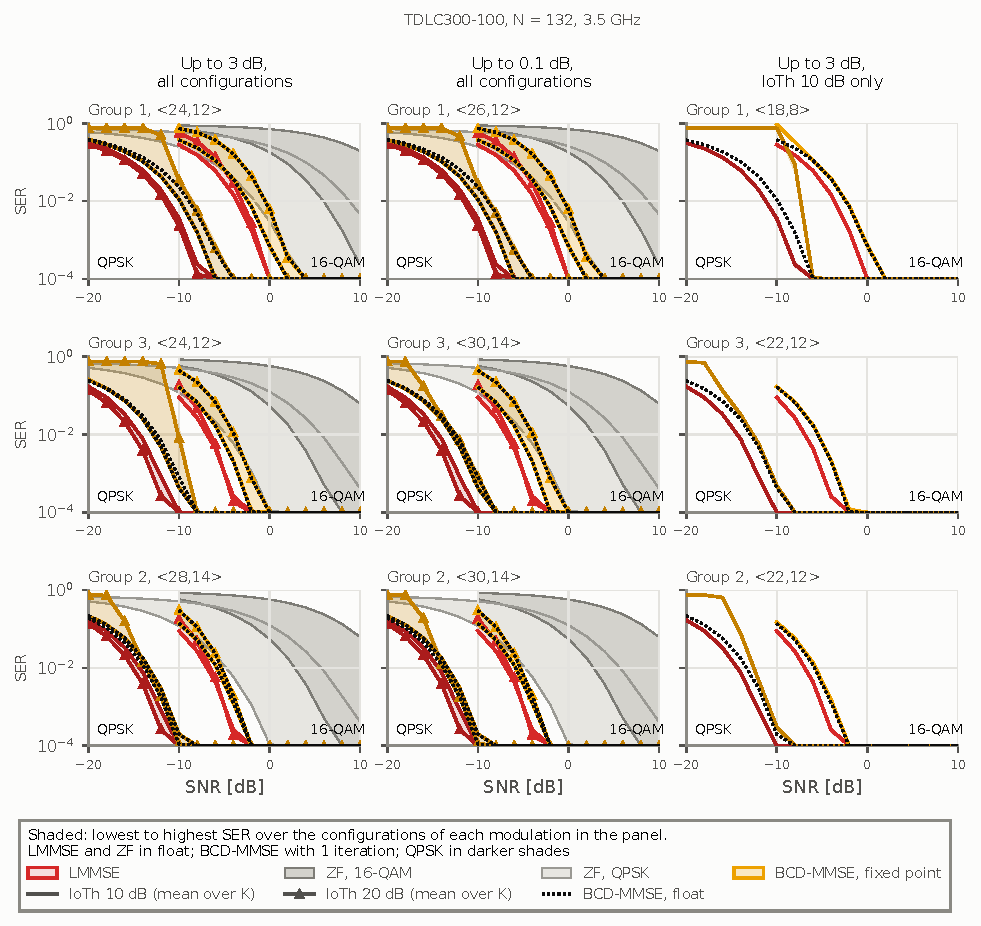
\includegraphics[width=\textwidth]{Images/RESULTADOS/curvas_ser/curvas_ser_grupos_range_C300.pdf}
\vspace{4pt}
\legend{\textcolor{red}{Fonte: a autora.}}
\end{figure}

Within a group, the configurations vary only in terms of soft constraints: modulation, $K$, and IoTh (Section~\ref{subsec:configuracoes-bs}). In each plot, the QPSK curves appear on the left in darker shades, while the 16-QAM curves appear on the right in lighter shades. The dotted line represents the floating-point BCD-MMSE, which serves as the reference for the format. Each curve represents the average between $K=8$ and $K=12$; these values differ by at most 0.9~dB at an SER of $10^{-2}$. The shaded region surrounding the curves spans from the lowest to the highest SER observed across the configurations of that modulation. Since $K$ has little impact, the width of this region in the first two columns primarily reflects the difference between IoTh values of 10~dB and 20~dB.

In floating-point arithmetic, QPSK operates at lower SNRs than 16-QAM (Section~\ref{subsec:simbolos}). In fixed-point arithmetic, however, some QPSK curves begin with a plateau: a flat, horizontal segment at the top of the plot, corresponding to an SER of 0.75. An SER of 0.75 implies that 3 out of every 4 symbols are incorrect, equivalent to a random selection among the 4 constellation points. Within this plateau, increasing the SNR does not improve the SER; beyond it, the curve drops sharply.

With a greater number of integer bits, the plateau ends at a lower SNR. In groups 1 and 2, the 0.1~dB format differs from the 3~dB format only by having more fractional bits, and the plateau ends at the same SNR. In group 3, the $\langle 30,14\rangle$ format has two more integer bits than the $\langle 24,12\rangle$ format, causing the plateau to end earlier. 16-QAM, on the other hand, operates at higher SNRs and shows almost no variation across the different formats. The exception is the $\langle 18,8\rangle$ format, where the 16-QAM curve begins above the floating-point curve, near $\mathrm{SER} = 1$, and quickly converges with it.

It should be noted that the LMMSE in the graphs is in floating point. Consequently, one cannot draw conclusions regarding how its performance varies with different IoTh values compared to the BCD-MMSE approach. It is observable, however, that the groups with smaller clusters (groups 1 and 3) exhibit the greatest gap between the BCD-MMSE curves for IoTh values of 10~dB and 20~dB, particularly when using 16-QAM (Figures~\ref{fig:descentralizacao-grupo1} and \ref{fig:descentralizacao-grupo3}).

Considering only the configurations with an IoTh of 10~dB, the 3~dB formats feature 2 to 6 fewer bits (Table~\ref{tab:formatos-escolhidos}). As shown in the third column, these formats remain within the 3~dB increase threshold at an $\mathrm{SER}$ of $10^{-2}$. Regarding the SNR increase of BCD-MMSE over LMMSE, no specific target was defined; nevertheless, this increase exceeds 3~dB only in the case of QPSK. This occurs in the smaller formats, $\langle 18,8\rangle$ for group 1 and $\langle 24,12\rangle$ for group 3, and, marginally, for the 1H configuration in $\langle 26,12\rangle$ (Figures~\ref{fig:descentralizacao-grupo1} and \ref{fig:descentralizacao-grupo3}). 

QPSK is the modulation scheme most sensitive to the number of bits because it operates at lower SNRs, where the elements of $\mathbf G_c$ are larger (Section~\ref{subsec:resultados-grupo2}). When these elements exceed the capacity of the chosen format, an integer overflow occurs, which results in a plateau (Section~\ref{subsubsec:ponto-fixo}). For instance, the $\langle 18,8\rangle$ format can store values up to 128. In the 1C case, the median of the largest element in $\mathbf G_c$ ranges from 70 at $-6$~dB to 164 at $-10$~dB. It exceeds the limit for nearly all matrices at $-10$~dB, while it does not exceed the limit for any matrix at $-6$~dB. It is within this range that the QPSK curve emerges from the plateau. Although the modulation scheme itself does not alter $\mathbf G_c$ (Section~\ref{subsec:hw-matrizes}), 16-QAM operates at higher SNRs, where such overflows occur less frequently.


% =====================================================================
% Arquiteturas de hardware (Resultados), por condição de teste.
% Esqueleto (2026-11-07). Dados: relatórios do servidor (Vivado 2023.2),
%   hardware/resultados_servidor/.
% Tabelas e números (2026-11-08): software/testes/analise_potencia_qualidade.py
%   (tabelas em hardware/resultados_servidor/tabelas/*.tex, números em .../tabelas/resumo.txt)
%   e figuras_potencia_servidor.py (potencia_media_condicao). As tabelas foram coladas aqui;
%   ao gerar de novo, comparar com o .tex do script.
% Figuras (2026-11-09; separadas em 2026-11-13): energia_inversao (energia_inversao_formatos) e
%   potencia_recursos (potencia_recursos_lado), ambas de figuras_potencia_servidor.py, e quadrantes_cond_g1/_g3 (analise_potencia_qualidade.py), copiadas em
%   Images/RESULTADOS. Tabela tab:escolha-condicao: tabelas/tabela_escolha_condicao.tex.
% 2026-11-09: conferido depois da rodada6 (grade inteira): tabelas e figuras iguais.
% =====================================================================
% Sem isto, as figuras da seção de formatos (grupo 3 e perfis) saíam no meio desta seção.
% 2026-11-11: \FloatBarrier no lugar do \clearpage, que deixava a figura dos perfis sozinha
%   numa página.
\FloatBarrier
\section{\texorpdfstring{\textcolor{red}{Arquiteturas de hardware}}{Arquiteturas de hardware}}\label{sec:resultados-hardware}

% 2026-11-13: seção reorganizada a pedido da autora. Introdução nova; recursos primeiro por
%   arquitetura, na ordem da Metodologia (subsec:hw-arquiteturas), com o recurso mais usado e o
%   motivo; depois as tabelas e a comparação geral. Backup: scratchpad da sessão 8a590fec.
% FONTE da introdução: Tabela tab:recursos-faixa (intervalo x limite; caminho crítico).

\textcolor{red}{Esta seção mostra os resultados de implementação das arquiteturas no XCU50, a 100~MHz. Em todos os formatos, nas arquiteturas otimizadas, o intervalo entre duas inversões fica abaixo do limite de ciclos da Tabela~\ref{tab:limite-ciclos}. O módulo aceita um bloco novo de 275 matrizes a cada $T_c$ e acompanha a chegada das amostras. O timing é alcançado em todas as arquiteturas, com maior caminho crítico de 9,74~ns, na TDLB100-400.}

\textcolor{red}{A Seção~\ref{subsec:resultados-recursos-arquitetura} analisa os recursos de cada arquitetura, na mesma ordem da Seção~\ref{subsec:hw-arquiteturas}, e mostra qual recurso cada uma mais usa e por quê. A Seção~\ref{subsec:resultados-recursos} compara as arquiteturas e os formatos, e a Seção~\ref{subsec:resultados-potencia} mostra a potência e a energia por inversão.}

% ---------------------------------------------------------------------
\subsection{\texorpdfstring{\textcolor{red}{Recursos por arquitetura}}{Recursos por arquitetura}}\label{subsec:resultados-recursos-arquitetura}
% ---------------------------------------------------------------------
\textcolor{red}{A Figura~\ref{fig:recursos-faixa-arquitetura} mostra o uso de cada recurso em cada arquitetura, em porcentagem do XCU50. Cada traço vai do menor ao maior uso entre os formatos. O recurso mais usado de cada arquitetura é o traço mais alto do grupo. Nas seções a seguir, cada arquitetura é comparada com a anterior. Quando o texto diz, por exemplo, que as LUTs crescem de 4,6 a 6,8 vezes, a conta é feita com o mesmo formato nas duas arquiteturas, e a faixa vai do formato que cresce menos ao que cresce mais (Tabelas~\ref{tab:recursos} e \ref{tab:recursos-sem-otimizacao}).}

\begin{figure}[!ht]
\caption{\textcolor{red}{Uso de cada recurso do XCU50 por arquitetura, do menor ao maior entre os formatos.}}
\label{fig:recursos-faixa-arquitetura}
\vspace{4pt} % a classe zera o espaço entre a caption e a figura
\centering
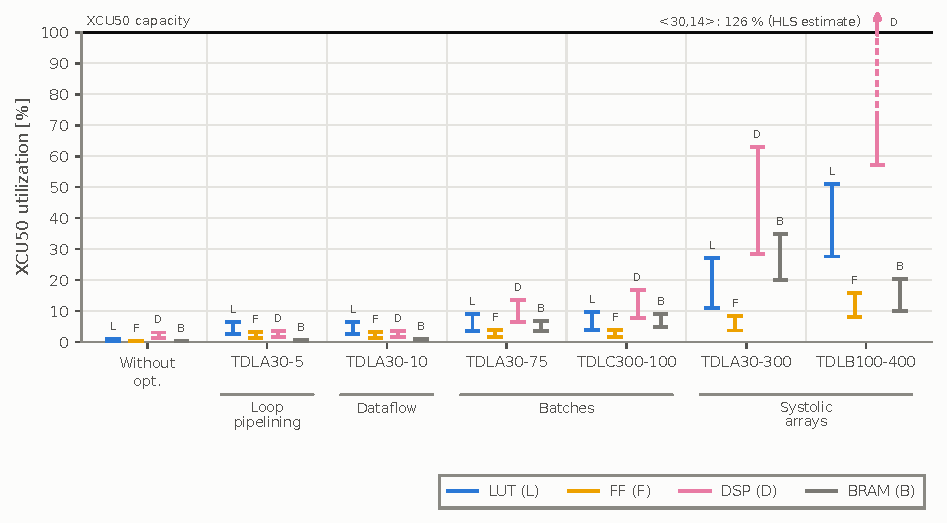
\includegraphics[width=\textwidth]{Images/RESULTADOS/recursos_faixa_arquitetura.pdf}
\vspace{4pt}
\legend{\textcolor{red}{Fonte: a autora. Circuito $16 \times 16$. No DSP da TDLB100-400, a seta indica que o $\langle 30,14\rangle$ passa da capacidade do XCU50: a estimativa do HLS é de 126\%, e ele não cabe no FPGA.}}
\end{figure}

% ---------------------------------------------------------------------
\subsubsection{\texorpdfstring{\textcolor{red}{Pipeline de laços}}{Pipeline de laços}}\label{subsubsec:resultados-pipeline-lacos}
% ---------------------------------------------------------------------
\textcolor{red}{Na versão sem otimização, o recurso mais usado são os DSPs, com 1,4 a 3,1\%. A arquitetura da TDLA30-5 reduz o intervalo de 3,6 a 4,5 vezes. Os DSPs crescem só de 1,1 a 1,2 vez, mas as LUTs crescem de 4,6 a 6,8 vezes, e os FFs, de 9,4 a 13,2 vezes. Com isso, o recurso mais usado passa a ser a LUT, com 2,5 a 6,6\%.}

\textcolor{red}{Esse aumento vem dos divisores. No relatório do HLS, os divisores da versão sem otimização são sequenciais: cada um faz uma divisão por vez e só aceita a próxima quando termina. Com o pipeline de laços, o laço da divisão começa uma iteração por ciclo, e o HLS usa divisores em pipeline, que aceitam uma divisão por ciclo. O único relatório do HLS com o uso de cada operador dessa arquitetura é o de palavras de 24 bits. Nele, os quatro divisores da LU e da substituição direta somam 91\% dos FFs e 71\% das LUTs, e nenhum DSP.}

% ---------------------------------------------------------------------
\subsubsection{\texorpdfstring{\textcolor{red}{Dataflow entre etapas}}{Dataflow entre etapas}}\label{subsubsec:resultados-dataflow}
% ---------------------------------------------------------------------
\textcolor{red}{A arquitetura da TDLA30-10 reduz o intervalo mais 2,5 a 2,7 vezes, e as LUTs, os FFs e os DSPs não mudam. O dataflow não cria operadores novos (Seção~\ref{subsubsec:hw-dataflow}). O custo fica na memória, e as BRAMs crescem de 1,3 a 1,7 vez. Entre as etapas, o HLS usa buffers ping-pong, que guardam cada matriz pelo menos duas vezes~\cite[p.~115]{kastner-hls}. Como os divisores são os mesmos, o recurso mais usado continua sendo a LUT, com 2,5 a 6,5\%.}

% ---------------------------------------------------------------------
\subsubsection{\texorpdfstring{\textcolor{red}{Lotes de matrizes}}{Lotes de matrizes}}\label{subsubsec:resultados-lotes}
% ---------------------------------------------------------------------
\textcolor{red}{Com lote, as BRAMs seguem o número de bancos de memória, e não o número de matrizes guardadas. Cada banco ocupa pelo menos um bloco de BRAM, mesmo quando guarda poucas palavras.}

\textcolor{red}{Na TDLA30-75, com 6 cópias, o intervalo por matriz é de 5,7 a 6,3 vezes menor que na TDLA30-10. Os DSPs crescem de 3,6 a 3,8 vezes, e as LUTs, só de 1,3 a 1,5 vez. Os multiplicadores das atualizações são copiados 6 vezes, mas o divisor de cada etapa é um só para as cópias (Seção~\ref{subsubsec:hw-lotes}). Assim, a parte do circuito que mais usa LUTs não é copiada. As BRAMs crescem de 6,9 a 8,2 vezes, porque cada matriz passa a ficar em 6 bancos, um por cópia. Da TDLA30-75 para a TDLC300-100, as cópias vão de 6 para 8, e as BRAMs crescem na mesma proporção, 1,33 vez, em todos os formatos.}

\textcolor{red}{Assim, a BRAM e os DSPs ficam próximos, e o recurso mais usado depende do formato. Do $\langle 20,8\rangle$ ao $\langle 24,12\rangle$, é a BRAM, com 6,7\% na TDLA30-75 e 8,9\% na TDLC300-100. No $\langle 18,8\rangle$, essas arquiteturas usam cerca de metade das BRAMs dos outros formatos, e a partir do $\langle 26,12\rangle$, os DSPs crescem. Nesses formatos, o recurso mais usado são os DSPs.}

% DSP x formato (2026-11-13): larguras dos multiplicadores nos RTL dos pacotes (pacote_servidor_formatos*/
%   versoes/<fmt>_<arq>/rtl/*mul_*): 28 (<18,8>), 32 (<20,8>, <22,12>), 36 (<24,12>), 40 (<26,12>),
%   42 (<28,14>), 46 (<30,14>) bits; iguais na 606 e na 152. DSPs por multiplicador no csynth.rpt:
%   mul_36s_36s = 4 (cholesky_hardware_diretivas_606/sintese, pacote_servidor_2023/_montagem/152);
%   mul_46s_46s = 9 (viabilidade_30_14/152_sistolico). Sem relatório com DSPs por multiplicador em 40 e 42 bits.
%   UG1399 p. 499 (página do PDF): multiplicação mais larga que o necessário usa vários módulos DSP.
\textcolor{red}{Os DSPs crescem com o formato porque os multiplicadores ficam mais largos. Nos relatórios do HLS, os operandos dos multiplicadores das atualizações têm 28 bits no $\langle 18,8\rangle$, 36 bits no $\langle 24,12\rangle$ e 46 bits no $\langle 30,14\rangle$. Uma multiplicação mais larga é feita com vários DSPs~\cite[p.~499]{ug1399}. Do $\langle 18,8\rangle$ ao $\langle 24,12\rangle$, o total de DSPs quase não muda, e no relatório do $\langle 24,12\rangle$ cada multiplicador usa 4 DSPs. A partir do $\langle 26,12\rangle$, com 40 bits, o total cresce. No $\langle 30,14\rangle$, cada multiplicador usa 9 DSPs.}

% ---------------------------------------------------------------------
\subsubsection{\texorpdfstring{\textcolor{red}{Arranjos sistólicos}}{Arranjos sistólicos}}\label{subsubsec:resultados-sistolico}
% ---------------------------------------------------------------------
\textcolor{red}{Na TDLA30-300, com só 2 cópias, o intervalo é de 3,0 a 3,3 vezes menor que na TDLC300-100. Em cada etapa, as 2 cópias somam 32 multiplicadores, um por PE, contra 8 na TDLC300-100, e cada cópia tem o seu divisor (Seção~\ref{subsubsec:hw-sistolico}). Os DSPs crescem de 3,7 a 3,8 vezes, e as LUTs, de 2,7 a 2,9 vezes. Cada linha da matriz fica em 16 bancos, um por PE, e cada cópia tem os seus. Assim, as BRAMs crescem de 3,8 a 4,2 vezes. No relatório do HLS de palavras de 24 bits, cada um desses bancos ocupa um bloco de 18~Kb, mas guarda só 256 palavras, cerca de um terço do bloco. Como na TDLC300-100, o recurso mais usado é a BRAM do $\langle 20,8\rangle$ ao $\langle 24,12\rangle$, com 34,2 a 34,4\%, e os DSPs nos outros formatos. Os multiplicadores são os mesmos dos lotes, e os DSPs crescem com o formato pelo mesmo motivo (Seção~\ref{subsubsec:resultados-lotes}). Mas, como a TDLA30-300 já usa muitos DSPs, esse crescimento pesa mais no FPGA: os DSPs vão de 28,6\% no $\langle 24,12\rangle$ para 63,1\% no $\langle 30,14\rangle$.}

\textcolor{red}{Na TDLB100-400, as cópias vão de 2 para 4, e o intervalo cai à metade, de 128 para 64 ciclos. Os DSPs também dobram. As LUTs crescem de 2,4 a 2,5 vezes, e as BRAMs caem quase à metade. Com 4 cópias, cada banco guarda metade das palavras, e o HLS fez esses bancos em LUTs, e não em BRAM. Uma memória pode ser feita em BRAM, em LUTs (LUTRAM) ou em URAM~\cite[p.~53]{ug1399}. No relatório do Vivado, as LUTs usadas como memória crescem de 7,4 a 9,8 vezes, e as LUTs de lógica, 2,0 vezes, como as cópias. Assim, em todos os formatos, o recurso mais usado são os DSPs, com 57,1 a 72,4\%, e as BRAMs ficam entre 10,0 e 20,2\%.}

% ---------------------------------------------------------------------
\subsection{\texorpdfstring{\textcolor{red}{Comparação entre as arquiteturas}}{Comparação entre as arquiteturas}}\label{subsec:resultados-recursos}
% ---------------------------------------------------------------------
% FONTE: resultados_vivado_servidor.csv (relatório de implementação, utilizacao.rpt); totais do
%   XCU50 do próprio utilizacao.rpt: 871.680 LUT, 1.743.360 FF, 5.952 DSP, 1.344 blocos de
%   36 Kb (2.688 de 18 Kb). 7.512 DSP do <30,14> na 114: coluna observacao do CSV.

\textcolor{red}{A Tabela~\ref{tab:recursos-faixa} mostra o melhor e o pior caso de cada arquitetura entre os formatos: o menor e o maior uso de cada recurso, de caminho crítico e de intervalo entre inversões. Os valores de cada formato estão nas Tabelas~\ref{tab:recursos} e \ref{tab:recursos-sem-otimizacao} (Apêndice~\ref{ap:recursos}).}

\textcolor{red}{As arquiteturas sem lote (TDLA30-5 e TDLA30-10) usam no máximo 6,6\% de cada recurso, e a versão sem otimização, no máximo 3,1\%. Em $32 \times 32$, a versão sem otimização usa quase os mesmos recursos que em $16 \times 16$, mas o intervalo cresce de 5 a 6 vezes.}

\begin{table}[htbp]
\caption{\textcolor{red}{Menor e maior uso de recursos, caminho crítico e intervalo entre inversões de cada arquitetura, entre os formatos.}}
\label{tab:recursos-faixa}
\vspace{4pt} % a classe zera o espaço entre a caption e a tabela
\centering
\footnotesize
\color{red}
\renewcommand{\arraystretch}{1.2}
\setlength{\tabcolsep}{2pt}
\begin{tabular}{lccccccc}
\toprule
\textbf{Test condition} & \textbf{LUT (\%)} & \textbf{FF (\%)} & \textbf{DSP (\%)} & \textbf{BRAM (\%)} & \begin{tabular}[c]{@{}c@{}}\textbf{Critical}\\\textbf{path (ns)}\end{tabular} & \begin{tabular}[c]{@{}c@{}}\textbf{Interval}\\\textbf{(cycles)}\end{tabular} & \begin{tabular}[c]{@{}c@{}}\textbf{Limit}\\\textbf{(cycles)}\end{tabular} \\
\midrule
TDLA30-5 & 2.5--6.6 & 1.2--3.2 & 1.7--3.7 & 0.4--0.6 & 7.24--9.03 & 7,081--8,627 & 9,090 \\
TDLA30-10 & 2.5--6.5 & 1.2--3.3 & 1.7--3.7 & 0.5--0.9 & 7.54--8.36 & 2,765--3,320 & 4,545 \\
TDLA30-75 & 3.7--9.0 & 1.6--4.0 & 6.3--13.5 & 3.6--6.7 & 7.87--8.98 & 483.9--528.9 & 606 \\
TDLC300-100 & 4.0--9.7 & 1.6--4.0 & 7.7--16.9 & 4.8--8.9 & 7.79--9.37 & 387.3--421.1 & 454 \\
TDLA30-300 & 11.0--27.2 & 3.7--8.5 & 28.6--63.1 & 20.0--35.0 & 8.73--9.66 & 128 & 151 \\
TDLB100-400 & 27.6--51.0 & 8.0--15.9 & 57.1--72.4 & 10.0--20.2 & 9.38--9.74 & 64 & 113 \\
\midrule
Without opt., 16 $\times$ 16 & 0.5--1.0 & 0.1--0.2 & 1.4--3.1 & 0.3--0.5 & 7.80--9.15 & 26,702--38,567 & -- \\
Without opt., 32 $\times$ 32 & 0.5--1.0 & 0.1--0.3 & 1.4--3.1 & 0.3--0.7 & 7.72--8.58 & 159,086--194,367 & -- \\
\bottomrule
\end{tabular}
\vspace{4pt}
\legend{\textcolor{red}{Fonte: a autora. Recursos em porcentagem do XCU50. Em quase todos os casos, o menor valor vem do $\langle 18,8\rangle$ e o maior, do $\langle 30,14\rangle$ ($\langle 28,14\rangle$ na TDLB100-400). O caminho crítico não segue essa ordem. Em $32 \times 32$, sem o intervalo do $\langle 18,8\rangle$ e do $\langle 20,8\rangle$, que não foram medidos.}}
\end{table}

\textcolor{red}{A Tabela~\ref{tab:recurso-mais-usado} mostra o recurso mais usado em cada formato. O maior efeito do formato está no $\langle 30,14\rangle$, em que os DSPs quase dobram em relação ao $\langle 28,14\rangle$: na TDLA30-300, vão de 36 para 63\%. Na TDLB100-400, o $\langle 30,14\rangle$ não cabe no FPGA: a estimativa do HLS é de 7.512 DSPs, e o XCU50 tem 5.952.}

\begin{table}[htbp]
\caption{\textcolor{red}{Recurso mais usado do XCU50, em porcentagem, por formato e arquitetura.}}
\label{tab:recurso-mais-usado}
\vspace{4pt} % a classe zera o espaço entre a caption e a tabela
\centering
\footnotesize
\color{red}
\renewcommand{\arraystretch}{1.2}
\setlength{\tabcolsep}{4pt}
\begin{tabular}{lcccccccc}
\toprule
\textbf{Test condition} & \textbf{$\langle 18,8\rangle$} & \textbf{$\langle 18,8\rangle$$^{*}$} & \textbf{$\langle 20,8\rangle$} & \textbf{$\langle 22,12\rangle$} & \textbf{$\langle 24,12\rangle$} & \textbf{$\langle 26,12\rangle$} & \textbf{$\langle 28,14\rangle$} & \textbf{$\langle 30,14\rangle$$^{*}$} \\
\midrule
TDLA30-5 & 2.5 (L) & 2.6 (L) & 3.2 (L) & 3.2 (L) & 4.1 (L) & 4.9 (L) & 5.4 (L) & 6.6 (L) \\
TDLA30-10 & 2.5 (L) & 2.6 (L) & 3.2 (L) & 3.3 (L) & 4.1 (L) & 5.0 (L) & 5.5 (L) & 6.5 (L) \\
TDLA30-75 & 6.3 (D) & 6.3 (D) & 6.7 (B) & 6.7 (B) & 6.7 (B) & 7.7 (D) & 7.9 (D) & 13.5 (D) \\
TDLC300-100 & 7.7 (D) & 7.7 (D) & 8.9 (B) & 8.9 (B) & 8.9 (B) & 9.4 (D) & 9.7 (D) & 16.9 (D) \\
TDLA30-300 & 28.6 (D) & 28.6 (D) & 34.2 (B) & 34.3 (B) & 34.4 (B) & 35.1 (D) & 36.2 (D) & 63.1 (D) \\
TDLB100-400 & 57.2 (D) & 57.2 (D) & 57.6 (D) & 57.3 (D) & 57.1 (D) & 70.3 (D) & 72.4 (D) & -- \\
\bottomrule
\end{tabular}
\vspace{4pt}
\legend{\textcolor{red}{Fonte: a autora. Entre parênteses, o recurso: L = LUT, D = DSP, B = BRAM. $^{*}$\texttt{AP\_TRN}/\texttt{AP\_SAT}; os outros, \texttt{AP\_RND\_ZERO}/\texttt{AP\_WRAP}. --: não cabe no FPGA.}}
\end{table}

% Ocupação formato a formato (tab:recurso-mais-usado): TDLA30-10 -> TDLA30-75 cresce 1,4 a 2,5 vezes;
%   TDLA30-300 -> TDLB100-400, 1,7 a 2,0 vezes.
\textcolor{red}{O gráfico da esquerda da Figura~\ref{fig:potencia-recursos} mostra o recurso mais usado. Como ele muda de uma arquitetura para outra, a ocupação não segue o limite de ciclos. Da TDLA30-10 para a TDLA30-75, o limite fica 7,5 vezes menor, e a ocupação cresce só de 1,4 a 2,5 vezes. Da TDLA30-300 para a TDLB100-400, o limite fica só 1,3 vez menor, e a ocupação cresce de 1,7 a 2,0 vezes.}

% ---------------------------------------------------------------------
\subsection{\texorpdfstring{\textcolor{red}{Potência e energia}}{Potência e energia}}\label{subsec:resultados-potencia}
% ---------------------------------------------------------------------
% FONTE: resultados_vivado_servidor.csv (report_power com SAIF); estática = total - dinâmica
%   (2,212 a 2,300 W em todas as linhas 16 x 16). Inclinação e razões: tabelas/resumo.txt.
%   Figura da potência média no ritmo (potencia_media_condicao) retirada em 2026-11-09, a
%   pedido da autora: a de potência dinâmica já mostra esses dados.

% Razão TDLB100-400 / TDLA30-5 formato a formato: 15,4 (<28,14>) a 20,0 (<18,8> TRN/SAT).
\textcolor{red}{A Tabela~\ref{tab:potencia-dinamica} mostra a potência dinâmica. Em cada formato, a da TDLB100-400 é de 15 a 20 vezes a da TDLA30-5. O formato pesa menos que a arquitetura. Do $\langle 18,8\rangle$ ao $\langle 28,14\rangle$, a potência dinâmica cresce de 1,6 a 2,0 vezes em cada arquitetura. Nesse intervalo, cada bit a mais na palavra custa, em média, 15~mW na TDLA30-5 e 180~mW na TDLB100-400. A potência estática fica entre 2,21 e 2,30~W em todas as arquiteturas e formatos.}


\begin{table}[htbp]
\caption{\textcolor{red}{Potência dinâmica, em W, por formato e arquitetura.}}
\label{tab:potencia-dinamica}
\vspace{4pt} % a classe zera o espaço entre a caption e a tabela
\centering
\footnotesize
\color{red}
\renewcommand{\arraystretch}{1.2}
\setlength{\tabcolsep}{3pt}
\begin{tabular}{lcccccccc}
\toprule
\textbf{Test condition} & \textbf{$\langle 18,8\rangle$} & \textbf{$\langle 18,8\rangle$$^{*}$} & \textbf{$\langle 20,8\rangle$} & \textbf{$\langle 22,12\rangle$} & \textbf{$\langle 24,12\rangle$} & \textbf{$\langle 26,12\rangle$} & \textbf{$\langle 28,14\rangle$} & \textbf{$\langle 30,14\rangle$$^{*}$} \\
\midrule
TDLA30-5 & 0.151 & 0.158 & 0.187 & 0.194 & 0.234 & 0.280 & 0.305 & 0.377 \\
TDLA30-10 & 0.209 & 0.208 & 0.252 & 0.253 & 0.305 & 0.362 & 0.391 & 0.496 \\
TDLA30-75 & 0.369 & 0.400 & 0.450 & 0.474 & 0.546 & 0.618 & 0.647 & 0.868 \\
TDLC300-100 & 0.452 & 0.482 & 0.570 & 0.573 & 0.666 & 0.759 & 0.805 & 1.037 \\
TDLA30-300 & 1.368 & 1.425 & 1.679 & 1.753 & 1.973 & 2.087 & 2.180 & 3.065 \\
TDLB100-400 & 2.908 & 3.167 & 3.313 & 3.477 & 4.062 & 4.456 & 4.703 & -- \\
\midrule
Without opt., 16 $\times$ 16 & 0.031 & 0.034 & 0.035 & 0.037 & 0.041 & 0.046 & 0.048 & 0.059 \\
Without opt., 32 $\times$ 32 & -- & -- & -- & 0.040 & 0.046 & 0.051 & 0.053 & 0.065 \\
\bottomrule
\end{tabular}
\vspace{4pt}
\legend{\textcolor{red}{Fonte: a autora. Arquitetura de cada condição de teste em $16 \times 16$. $^{*}$\texttt{AP\_TRN}/\texttt{AP\_SAT}; os outros, \texttt{AP\_RND\_ZERO}/\texttt{AP\_WRAP}. --: sem medida ou não cabe no FPGA.}}
\end{table}

% Faixas formato a formato (resultados_vivado_servidor.csv): com lote 1,75 a 4,59 uJ; TDLA30-5 /
%   maior e menor com lote no mesmo formato: 5,7 a 8,8; TDLA30-10 / TDLA30-5: 0,50 a 0,54.
\textcolor{red}{A Tabela~\ref{tab:energia-inversao} e a Figura~\ref{fig:energia-inversao} mostram a energia por inversão. Nas arquiteturas com lote, ela fica entre 1,75 e 4,59~$\mu$J, e as quatro ficam próximas em cada formato. A da TDLA30-5 gasta de 5,7 a 8,8 vezes mais que elas, no mesmo formato. Ela tem a menor potência dinâmica, mas cada inversão leva de 7.081 a 8.627 ciclos, contra 64 a 529 nas arquiteturas com lote. A da TDLA30-10 gasta cerca de metade da TDLA30-5.}


\begin{table}[htbp]
\caption{\textcolor{red}{Energia por inversão, em $\mu$J, por formato e arquitetura.}}
\label{tab:energia-inversao}
\vspace{4pt} % a classe zera o espaço entre a caption e a tabela
\centering
\footnotesize
\color{red}
\renewcommand{\arraystretch}{1.2}
\setlength{\tabcolsep}{3pt}
\begin{tabular}{lcccccccc}
\toprule
\textbf{Test condition} & \textbf{$\langle 18,8\rangle$} & \textbf{$\langle 18,8\rangle$$^{*}$} & \textbf{$\langle 20,8\rangle$} & \textbf{$\langle 22,12\rangle$} & \textbf{$\langle 24,12\rangle$} & \textbf{$\langle 26,12\rangle$} & \textbf{$\langle 28,14\rangle$} & \textbf{$\langle 30,14\rangle$$^{*}$} \\
\midrule
TDLA30-5 & 10.69 & 11.60 & 13.74 & 14.25 & 17.77 & 21.96 & 24.66 & 32.52 \\
TDLA30-10 & 5.81 & 5.75 & 7.31 & 7.34 & 9.21 & 11.37 & 12.51 & 16.47 \\
TDLA30-75 & 1.79 & 1.94 & 2.22 & 2.34 & 2.75 & 3.18 & 3.36 & 4.59 \\
TDLC300-100 & 1.75 & 1.87 & 2.25 & 2.26 & 2.68 & 3.11 & 3.33 & 4.37 \\
TDLA30-300 & 1.75 & 1.82 & 2.15 & 2.24 & 2.52 & 2.67 & 2.79 & 3.92 \\
TDLB100-400 & 1.86 & 2.03 & 2.12 & 2.23 & 2.60 & 2.85 & 3.01 & -- \\
\midrule
Without opt., 16 $\times$ 16 & 8.28 & 9.09 & 10.64 & 11.25 & 13.31 & 15.81 & 17.00 & 22.75 \\
Without opt., 32 $\times$ 32 & -- & -- & -- & 63.63 & 76.96 & 89.24 & 94.92 & 126.34 \\
\bottomrule
\end{tabular}
\vspace{4pt}
\legend{\textcolor{red}{Fonte: a autora. Cálculo na Seção~\ref{subsec:hw-potencia}. $^{*}$\texttt{AP\_TRN}/\texttt{AP\_SAT}; os outros, \texttt{AP\_RND\_ZERO}/\texttt{AP\_WRAP}. --: sem medida ou não cabe no FPGA.}}
\end{table}

\begin{figure}[!ht]
\caption{\textcolor{red}{Energia por inversão por formato e condição de teste.}}
\label{fig:energia-inversao}
\vspace{4pt} % a classe zera o espaço entre a caption e a figura
\centering
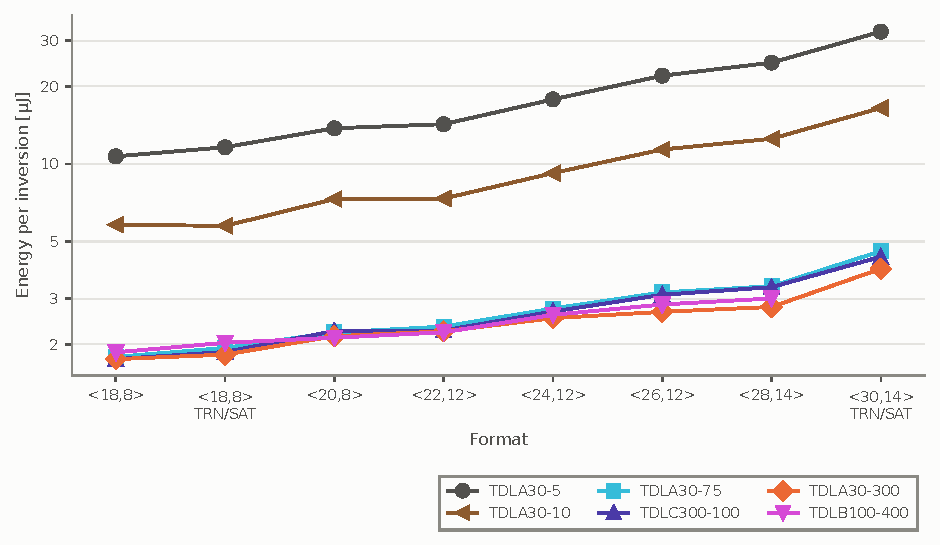
\includegraphics[width=\textwidth]{Images/RESULTADOS/energia_inversao.pdf}
\vspace{4pt}
\legend{\textcolor{red}{Fonte: a autora. Eixo vertical em escala logarítmica. Sem TRN/SAT no rótulo, o formato usa \texttt{AP\_RND\_ZERO}/\texttt{AP\_WRAP}. O $\langle 30,14\rangle$ da TDLB100-400 não cabe no FPGA.}}
\end{figure}

% FONTE: potencia_recursos_lado_data.csv (dinamica_sobre_estatica_pct, ocupacao_pct).
\textcolor{red}{A Figura~\ref{fig:potencia-recursos} junta, por formato, a ocupação do recurso mais usado (Tabela~\ref{tab:recurso-mais-usado}) e a potência dinâmica. Da TDLA30-5 à TDLC300-100, a potência dinâmica fica entre 7 e 46\% da estática. Na TDLA30-300, ela vai de 61 a 135\%, e na TDLB100-400, de 128 a 204\%.}


\begin{figure}[!ht]
\caption{\textcolor{red}{Ocupação do recurso mais usado do XCU50 (esquerda) e potência dinâmica (direita), por formato e condição de teste.}}
\label{fig:potencia-recursos}
\vspace{4pt} % a classe zera o espaço entre a caption e a figura
\centering
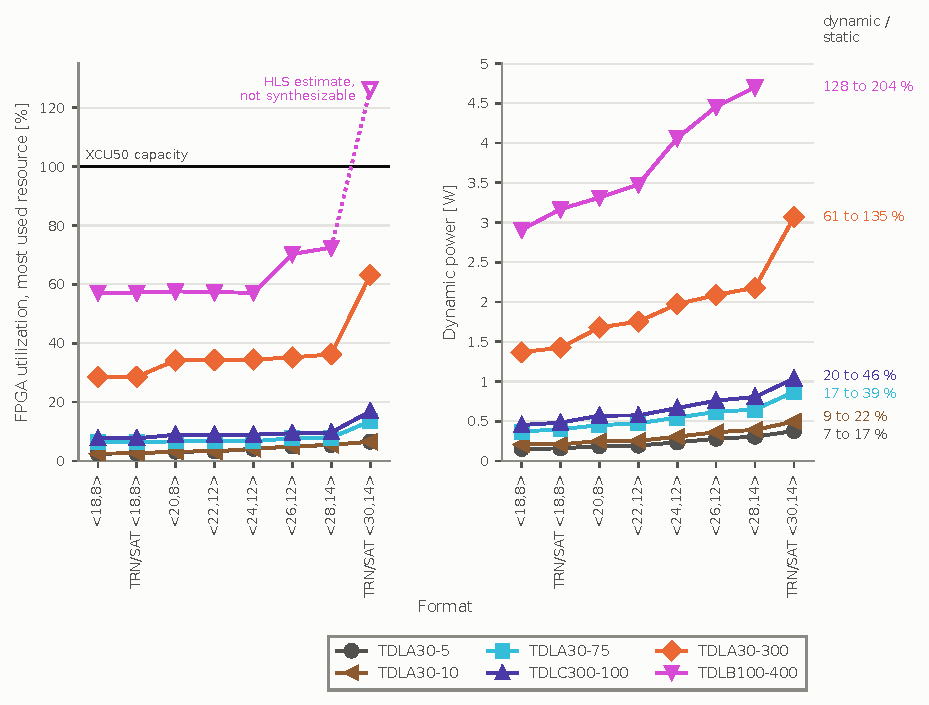
\includegraphics[width=\textwidth]{Images/RESULTADOS/potencia_recursos.pdf}
\vspace{4pt}
\legend{\textcolor{red}{Fonte: a autora. À direita, a potência dinâmica em porcentagem da estática, do menor ao maior formato. No $\langle 30,14\rangle$ da TDLB100-400, a ocupação é a estimativa do HLS.}}
\end{figure}


% =====================================================================
% RASCUNHO (2026-11-06): discussão de vazão e atraso, para a autora trabalhar.
%   Vem depois da seção de arquiteturas de hardware (RESULTADOS/hardware.tex).
% DADOS: hardware/resultados_servidor/atraso_por_bloco.xlsx (fórmulas) e
%   latencia_por_bloco.csv, gerados por hardware/latencia_por_bloco.py e
%   hardware/atraso_por_bloco_xlsx.py a partir dos logs xsim do servidor (Vivado 2023.2).
%   Os logs têm só 3 lotes (ou 20 matrizes); o intervalo sai de 2 (ou 19) medidas.
% A tabela mostra só <24,12>. Os outros formatos estão na planilha:
%   - a 455 passa de T_c de +3,2 % (<18,8>) a +11,5 % (<30,14>);
%   - a 152 passa de T_c por cerca de 21,5 % em todos;
%   - a folga da 606 cai de 11 % (<18,8>) para 3 % (<30,14>).
% =====================================================================
\section{\texorpdfstring{\textcolor{red}{Vazão e atraso}}{Vazão e atraso}}\label{sec:resultados-atraso}

% 2026-11-13: subseções Vazão e Atraso juntas. A vazão só confirmava o limite de ciclos, que já
%   está em subsec:resultados-recursos; ela virou uma frase no parágrafo depois da tabela.
\textcolor{red}{As arquiteturas foram feitas para o limite de vazão, e atender um limite de atraso ficou fora do escopo (Seção~\ref{subsec:restricao-vazao}). Esta seção mostra o atraso que resulta delas e por que ele não atende a latência prevista para o 5G. O atraso vai da chegada da primeira amostra de um bloco até a última inversão desse bloco. A primeira parte é a coleta das $N$ amostras (Seção~\ref{subsec:pipeline}). Com 48 REs de DM-RS por PRB e por slot, ela leva $\lceil N/48 \rceil$ slots, limitada a $T_c$. A segunda é o tempo para inverter o bloco (Equação~\ref{eq:fim-tarefas}). A Tabela~\ref{tab:atraso-bloco} mostra essas duas partes no formato $\langle 24, 12\rangle$.}

\begin{table}[!ht]
\caption{\textcolor{red}{Throughput and delay of one block of $N_{\text{PRB}} = 275$ inversions, format $\langle 24, 12\rangle$.}}
\label{tab:atraso-bloco}
\vspace{4pt} % a classe zera o espaço entre a caption e a tabela
\centering
\footnotesize
\color{red}
\renewcommand{\arraystretch}{1.2}
\setlength{\tabcolsep}{4pt}
\begin{tabular}{lccccc}
\toprule
\begin{tabular}[c]{@{}c@{}}\textbf{Test}\\\textbf{condition}\end{tabular} & \begin{tabular}[c]{@{}c@{}}{\boldmath $T_c$}\\\textbf{(ms)}\end{tabular} & \begin{tabular}[c]{@{}c@{}}\textbf{Block input}\\\textbf{(ms)}\end{tabular} & \begin{tabular}[c]{@{}c@{}}\textbf{Block end}\\\textbf{(ms)}\end{tabular} & \begin{tabular}[c]{@{}c@{}}\textbf{Collection}\\\textbf{(ms)}\end{tabular} & \begin{tabular}[c]{@{}c@{}}\textbf{Total delay}\\\textbf{(ms)}\end{tabular} \\
\midrule
TDLA30-5    & 25.000 & 20.884 & 20.884 & 2.000 & 22.884 \\
TDLA30-10   & 12.500 & 8.305  & 8.354  & 2.000 & 10.354 \\
TDLA30-75   & 1.667  & 1.391  & 1.543  & 0.500 & 2.043 \\
TDLC300-100 & 1.250  & 1.159  & 1.336  & 1.250 & 2.586 \\
TDLA30-300  & 0.417  & 0.369  & 0.506  & 0.417 & 0.923 \\
TDLB100-400 & 0.313  & 0.184  & 0.265  & 0.313 & 0.578 \\
\bottomrule
\end{tabular}
\vspace{4pt}
\legend{\textcolor{red}{Source: the author, from the netlist simulation at 100~MHz. Block input: time to accept the 275 matrices. Block end: time until the last inversion of the block. Total delay: collection plus block end.}}
\end{table}

\textcolor{red}{Como todas as arquiteturas atendem o limite de ciclos (Seção~\ref{sec:resultados-hardware}), o bloco inteiro entra no módulo antes de $T_c$, e não se forma fila. Nas condições TDLC300-100 e TDLA30-300, a última inversão do bloco termina depois de $T_c$. Esse excesso não se acumula, pois o bloco seguinte já entra no módulo a tempo. Ele é um atraso fixo, de cerca de uma latência de batch, e não uma perda de vazão. Além disso, cada PRB só precisa da sua própria inversão: os primeiros PRBs ficam prontos cerca de uma latência de batch depois da chegada do bloco, e o atraso da tabela é o do último PRB.}

\textcolor{red}{A ITU-R prevê que o IMT-2020 possa oferecer latência de 1~ms pela interface aérea \cite[p.~14]{itu-m2083}. Essa latência é a contribuição da rede de rádio para o tempo entre o envio e a recepção de um pacote \cite[p.~13]{itu-m2083}. O processamento na BS é uma das parcelas da latência do plano de usuário \cite[Sec.~7.2.6 e Tab.~3]{itu-m2412}. Só nas condições TDLA30-300 e TDLB100-400 o atraso fica abaixo de 1~ms. Nas outras, o atraso vai de 2,0 a 22,9~ms.}

\textcolor{red}{Parte desse atraso vem do método de estimação, e não do hardware. Com $N = 192$ em FR1, a coleta leva 4 slots de 0,5~ms, ou 2~ms, e já passa de 1~ms antes de qualquer inversão. A outra parte vem da escolha de projeto. As arquiteturas das condições de baixa mobilidade distribuem as 275 inversões por quase todo o $T_c$. Com isso, elas gastam menos área e potência (Seção~\ref{sec:resultados-hardware}), mas o último PRB fica pronto mais tarde. Uma arquitetura mais rápida reduziria essa parte do atraso, com mais área e potência. A arquitetura da TDLB100-400, por exemplo, termina um bloco em 0,27~ms.}

\textcolor{red}{A coleta também depende do PUSCH. O DM-RS só é transmitido junto com o PUSCH, e o PUSCH só ocupa os slots em que os UEs alvo foram escalonados (Seção~\ref{subsec:simbolos}). Este trabalho supõe que todo slot leva PUSCH. As bandas n78 e n257 usam TDD \cite[Tabs.~5.2-1 e 5.2-2]{3gpp-ts38104}, e só os slots de uplink levam o PUSCH. Com um padrão TDD real, os slots de uplink ficam mais espaçados. A coleta das $N$ amostras leva mais tempo ou, se passar de $T_c$, o número de amostras disponível diminui.}
% TODO: padrão TDD típico (sem fonte local). Se for usado um número, buscar a fonte.
% TODO: o valor de 4 ms para eMBB está no Rep. ITU-R M.2410-0, que não está em books/.


% Aumento de SNR x potência (Resultados), separado de hardware.tex em 2026-11-09 para fechar o
%   capítulo, como a última pergunta do roteiro da autora.
% =====================================================================
\section{\texorpdfstring{\textcolor{red}{Aumento de SNR e potência}}{Aumento de SNR e potência}}\label{subsec:resultados-compromisso}
% =====================================================================
% FONTE: analise_potencia_qualidade.py (quadrantes_cond_g1/_g3 e _data.csv,
%   tabela_escolha_condicao, escolha_cond). Qualidade: grade_inteira.py (mesmos dados das barras
%   e curvas). TDLA30-10 usa a simulação da TDLA30-5. Pior caso A-H = pior caso E-H em todos os
%   pontos dos grupos 1 e 3 (conferido no script). G1, <26,12>, TDLA30-5 e -10: 0,104 dB.

\textcolor{red}{As Figuras~\ref{fig:quadrantes-g1} e \ref{fig:quadrantes-g3} juntam o aumento de SNR e a potência dinâmica nos grupos 1 e 3. Cada ponto é um formato numa condição de teste. No eixo x, está o pior aumento de SNR entre as configurações do grupo com o IoTh do gráfico, naquela condição: 10~dB (A a D) à esquerda e 20~dB (E a H) à direita. No gráfico da direita, o pior caso é o mesmo de todo o grupo (A a H). No eixo y, está a potência dinâmica do formato na arquitetura da condição, e a linha horizontal marca a potência estática.}


\textcolor{red}{Só os grupos 1 e 3 aparecem, porque eles usam o circuito $16 \times 16$. No grupo 2 ($32 \times 32$), só a versão sem otimização foi implementada, e ela não atende nenhum limite. A potência foi medida só com matrizes do grupo 1 (Seção~\ref{subsec:hw-matrizes}), e isso é uma limitação para o grupo 3. Mas os dados de entrada parecem mudar pouco a potência: na versão sem otimização do $\langle 18,8\rangle$, medida com as matrizes de cada uma das 5 condições de teste, a potência dinâmica ficou entre 0,031 e 0,032~W.}


\begin{figure}[!ht]
\caption{\textcolor{red}{Aumento de SNR e potência dinâmica de cada formato nas condições de teste, grupo 1.}}
\label{fig:quadrantes-g1}
\vspace{4pt} % a classe zera o espaço entre a caption e a figura
\centering
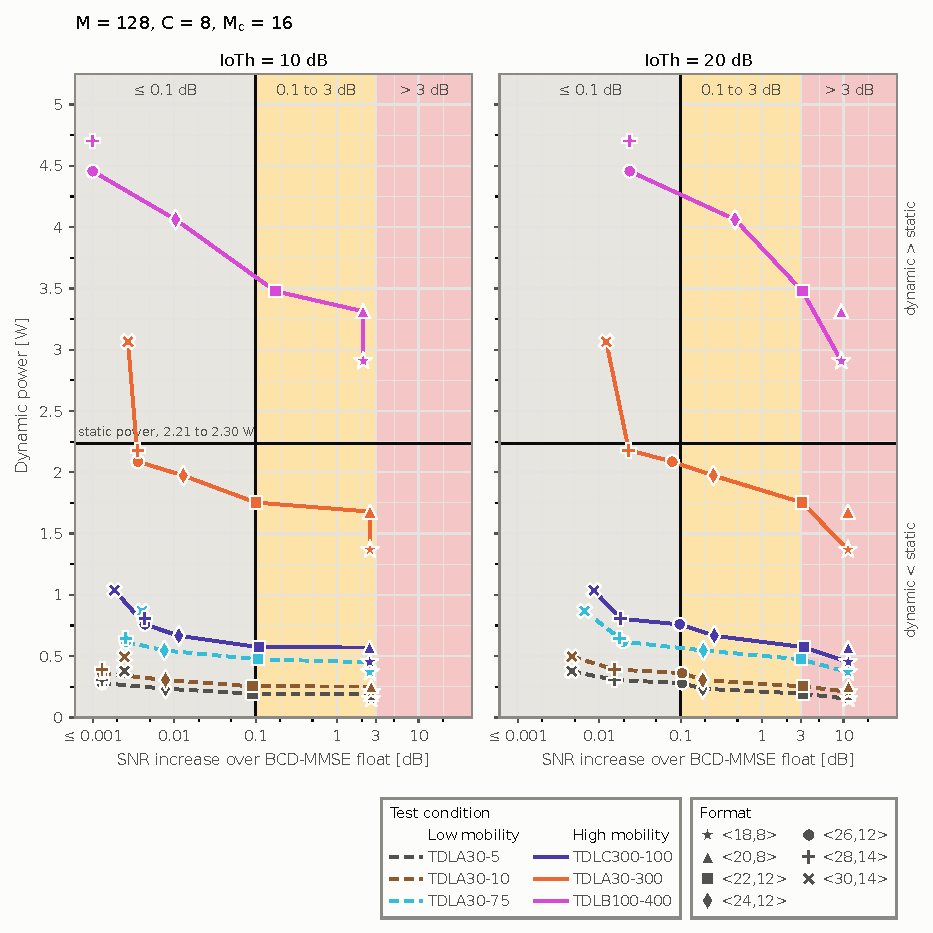
\includegraphics[width=\textwidth]{Images/RESULTADOS/quadrantes_cond_g1.pdf}
\vspace{4pt}
\legend{\textcolor{red}{Fonte: a autora. Linha tracejada: baixa mobilidade; cheia: alta mobilidade. As linhas ligam os formatos que nenhum outro supera ao mesmo tempo em aumento de SNR e em potência.}}
\end{figure}

\begin{figure}[!ht]
\caption{\textcolor{red}{Aumento de SNR e potência dinâmica de cada formato nas condições de teste, grupo 3.}}
\label{fig:quadrantes-g3}
\vspace{4pt} % a classe zera o espaço entre a caption e a figura
\centering
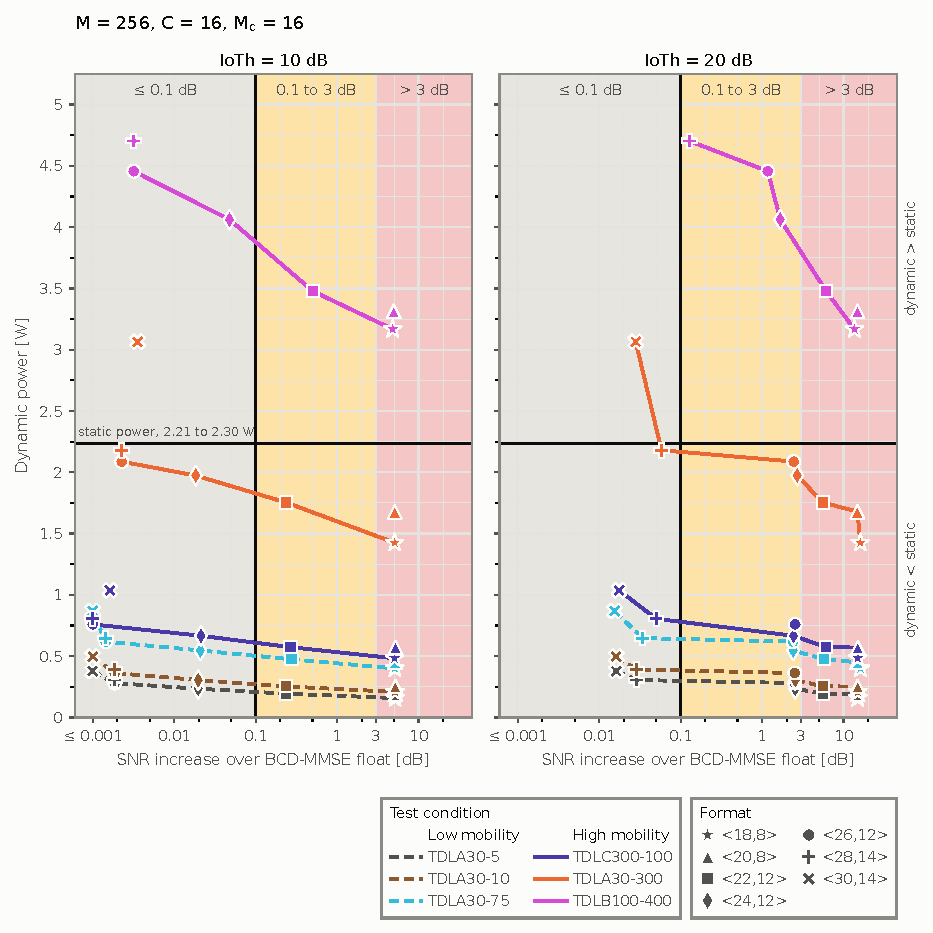
\includegraphics[width=\textwidth]{Images/RESULTADOS/quadrantes_cond_g3.pdf}
\vspace{4pt}
\legend{\textcolor{red}{Fonte: a autora. Linha tracejada: baixa mobilidade; cheia: alta mobilidade. As linhas ligam os formatos que nenhum outro supera ao mesmo tempo em aumento de SNR e em potência.}}
\end{figure}

\textcolor{red}{Como a potência muda mais com a arquitetura do que com o formato (Seção~\ref{subsec:resultados-potencia}), cada condição forma uma faixa de altura própria nas figuras. A Tabela~\ref{tab:escolha-condicao} mostra o formato escolhido em cada condição de teste: o menor que cabe na arquitetura e fica dentro do limite.}


\textcolor{red}{No grupo 1, com IoTh de 20~dB, o limite de 3~dB fica no $\langle 24,12\rangle$ em quase todas as condições. Na TDLA30-75, o $\langle 22,12\rangle$ já basta, com 2,97~dB. Para 0,1~dB, todas as condições usam o $\langle 26,12\rangle$. Na TDLA30-5 e na TDLA30-10, ele fica em 0,104~dB, que arredonda para 0,10~dB. Passar de 3~dB para 0,1~dB aumenta a potência dinâmica de 6\% (TDLA30-300) a 30\% (TDLA30-75).}


\textcolor{red}{Na TDLB100-400, o $\langle 24,12\rangle$ fica 0,47~dB acima do BCD-MMSE em ponto flutuante. Esse aumento pede que cada UE transmita 11\% mais energia por símbolo (Seção~\ref{subsec:aumento-snr}). O $\langle 26,12\rangle$ tira essa diferença com 0,39~W a mais de potência dinâmica no FPGA.}


\textcolor{red}{No grupo 3, com IoTh de 20~dB, o limite de 3~dB fica no $\langle 24,12\rangle$ em todas as condições. O de 0,1~dB fica no $\langle 28,14\rangle$, com 10 a 30\% mais potência dinâmica. Na TDLB100-400, nenhum formato que cabe no FPGA atende 0,1~dB. O $\langle 28,14\rangle$ fica em 0,13~dB, e o $\langle 30,14\rangle$ não cabe.}


\textcolor{red}{Com IoTh de 10~dB, os formatos ficam menores e só mudam entre as condições no grupo 1, para 0,1~dB: na TDLA30-5, na TDLA30-10 e na TDLA30-300, basta o $\langle 22,12\rangle$.}


\begin{table}[htbp]
\caption{\textcolor{red}{Formato escolhido em cada condição de teste, com o pior aumento de SNR, em dB, e a potência dinâmica, em W.}}
\label{tab:escolha-condicao}
\vspace{4pt} % a classe zera o espaço entre a caption e a tabela
\centering
\scriptsize
\color{red}
\renewcommand{\arraystretch}{1.2}
\setlength{\tabcolsep}{2.2pt}
\begin{tabular}{lcccccccccccc}
\toprule
 & \multicolumn{6}{c}{\textbf{IoTh of 10~dB (A to D)}} & \multicolumn{6}{c}{\textbf{IoTh of 20~dB (E to H)}} \\
\cmidrule(lr){2-7}\cmidrule(lr){8-13}
 & \multicolumn{3}{c}{\textbf{Up to 3 dB}} & \multicolumn{3}{c}{\textbf{Up to 0.1 dB}} & \multicolumn{3}{c}{\textbf{Up to 3 dB}} & \multicolumn{3}{c}{\textbf{Up to 0.1 dB}} \\
\cmidrule(lr){2-4}\cmidrule(lr){5-7}\cmidrule(lr){8-10}\cmidrule(lr){11-13}
\textbf{Test condition} & \textbf{Format} & \textbf{dB} & \textbf{W} & \textbf{Format} & \textbf{dB} & \textbf{W} & \textbf{Format} & \textbf{dB} & \textbf{W} & \textbf{Format} & \textbf{dB} & \textbf{W} \\
\midrule
\multicolumn{13}{l}{\textbf{Group 1 ($M$ = 128, $C$ = 8)}} \\
\multicolumn{13}{l}{Low mobility} \\
\quad TDLA30-5 & $\langle 18,8\rangle$ & 2.62 & 0.15 & $\langle 22,12\rangle$ & 0.09 & 0.19 & $\langle 24,12\rangle$ & 0.19 & 0.23 & $\langle 26,12\rangle$ & 0.10 & 0.28 \\
\quad TDLA30-10 & $\langle 18,8\rangle$ & 2.62 & 0.21 & $\langle 22,12\rangle$ & 0.09 & 0.25 & $\langle 24,12\rangle$ & 0.19 & 0.30 & $\langle 26,12\rangle$ & 0.10 & 0.36 \\
\quad TDLA30-75 & $\langle 18,8\rangle$ & 2.52 & 0.37 & $\langle 24,12\rangle$ & 0.01 & 0.55 & $\langle 22,12\rangle$ & 2.97 & 0.47 & $\langle 26,12\rangle$ & 0.02 & 0.62 \\
\multicolumn{13}{l}{High mobility} \\
\quad TDLC300-100 & $\langle 18,8\rangle$ & 2.51 & 0.45 & $\langle 24,12\rangle$ & 0.01 & 0.67 & $\langle 24,12\rangle$ & 0.26 & 0.67 & $\langle 26,12\rangle$ & 0.10 & 0.76 \\
\quad TDLA30-300 & $\langle 18,8\rangle$ & 2.53 & 1.37 & $\langle 22,12\rangle$ & 0.10 & 1.75 & $\langle 24,12\rangle$ & 0.25 & 1.97 & $\langle 26,12\rangle$ & 0.08 & 2.09 \\
\quad TDLB100-400 & $\langle 18,8\rangle$ & 2.09 & 2.91 & $\langle 24,12\rangle$ & 0.01 & 4.06 & $\langle 24,12\rangle$ & 0.47 & 4.06 & $\langle 26,12\rangle$ & 0.02 & 4.46 \\
\midrule
\multicolumn{13}{l}{\textbf{Group 3 ($M$ = 256, $C$ = 16)}} \\
\multicolumn{13}{l}{Low mobility} \\
\quad TDLA30-5 & $\langle 22,12\rangle$ & 0.23 & 0.19 & $\langle 24,12\rangle$ & 0.02 & 0.23 & $\langle 24,12\rangle$ & 2.55 & 0.23 & $\langle 28,14\rangle$ & 0.03 & 0.30 \\
\quad TDLA30-10 & $\langle 22,12\rangle$ & 0.23 & 0.25 & $\langle 24,12\rangle$ & 0.02 & 0.30 & $\langle 24,12\rangle$ & 2.55 & 0.30 & $\langle 28,14\rangle$ & 0.03 & 0.39 \\
\quad TDLA30-75 & $\langle 22,12\rangle$ & 0.28 & 0.47 & $\langle 24,12\rangle$ & 0.02 & 0.55 & $\langle 24,12\rangle$ & 2.40 & 0.55 & $\langle 28,14\rangle$ & 0.03 & 0.65 \\
\multicolumn{13}{l}{High mobility} \\
\quad TDLC300-100 & $\langle 22,12\rangle$ & 0.27 & 0.57 & $\langle 24,12\rangle$ & 0.02 & 0.67 & $\langle 24,12\rangle$ & 2.44 & 0.67 & $\langle 28,14\rangle$ & 0.05 & 0.81 \\
\quad TDLA30-300 & $\langle 22,12\rangle$ & 0.24 & 1.75 & $\langle 24,12\rangle$ & 0.02 & 1.97 & $\langle 24,12\rangle$ & 2.70 & 1.97 & $\langle 28,14\rangle$ & 0.06 & 2.18 \\
\quad TDLB100-400 & $\langle 22,12\rangle$ & 0.50 & 3.48 & $\langle 24,12\rangle$ & 0.05 & 4.06 & $\langle 24,12\rangle$ & 1.67 & 4.06 & -- & -- & -- \\
\bottomrule
\end{tabular}
\vspace{4pt}
\legend{\textcolor{red}{Fonte: a autora. Menor formato que cabe na arquitetura da condição de teste e cujo pior aumento de SNR, entre as configurações com aquele IoTh, fica até o limite. Modo \texttt{AP\_RND\_ZERO}/\texttt{AP\_WRAP}. --: nenhum formato que cabe no FPGA atende o limite.}}
\end{table}


\include{chapters/CONCLUSAO.tex}



% referências
% aqui será usado o environment padrao `thebibliography'; porém, sugere-se
% seriamente o uso de BibTeX e do estilo abnt.bst (veja na página do
% UTUG)
% 
% observe também o estilo meio estranho de alguns labels; isso é
% devido ao uso do pacote `natbib', que permite fazer citações de
% autores, ano, e diversas combinações desses

\bibliographystyle{abntex2-alf}
\bibliography{biblio}

% Apêndices (material da autora). Anexos (material de terceiros) usariam \annex.
\appendix
\chapter{Simulation parameters}\label{ap:parametros}
% =====================================================================
% APÊNDICE A -- só as tabelas de parâmetros da simulação.
% Movidas de RESULTADOS/setup_simulacao.tex em 2026-11-07, a pedido da autora.
% O texto e as seções continuam nos Resultados, citando estas tabelas.
% =====================================================================

\begin{table}[!ht]
\caption{Channel parameters set in the MATLAB script that runs QuaDRiGa.}
\label{tab:param_canal}
\vspace{4pt} % a classe zera o espaço entre a caption e a tabela
\centering
\footnotesize
\renewcommand{\arraystretch}{1.1}
\setlength{\aboverulesep}{0pt}
\setlength{\belowrulesep}{0pt}
\begin{tabular}{|p{2.7cm}|p{3.2cm}|p{4.2cm}|p{3.1cm}|}
\toprule
\centering\textbf{Source} & \centering\textbf{Parameter} & \centering\textbf{Name in the MATLAB script} & \centering\textbf{Value} \tabularnewline
\midrule
\multirow{5}{=}{\raggedright \citesp{zhao2025jsac}} & \raggedright Number of cells and BSs & \raggedright \texttt{tx\_\allowbreak{}position} (one BS) & \raggedright 1 \tabularnewline
\cline{2-4}
 & \raggedright Sector where the UEs are & \raggedright \texttt{sector\_\allowbreak{}deg} & \raggedright $120^\circ$ \tabularnewline
\cline{2-4}
 & \raggedright Position of the interferers & \raggedright \texttt{n\_\allowbreak{}ue = K + r} & \raggedright Same rule as the served UEs \tabularnewline
\cline{2-4}
 & \raggedright Channel generator & \raggedright -- & \raggedright QuaDRiGa \tabularnewline
\cline{2-4}
 & \raggedright Channel constant within a PRB & \raggedright -- & \raggedright Flat channel \tabularnewline
\midrule
\multirow{5}{=}{\raggedright QuaDRiGa default \citesp{quadriga-manual}} & \raggedright Uses only the minimal version of the 3GPP model & \raggedright \texttt{use\_\allowbreak{}3GPP\_\allowbreak{}baseline} & \raggedright \texttt{false} \tabularnewline
\cline{2-4}
 & \raggedright Shape of the spatial correlation of the large-scale parameters & \raggedright \texttt{autocorrelation\_\allowbreak{}function} & \raggedright \texttt{Comb300} \tabularnewline
\cline{2-4}
 & \raggedright Adds the direct-path delay to the delays & \raggedright \texttt{use\_\allowbreak{}absolute\_\allowbreak{}delays} & \raggedright \texttt{false} \tabularnewline
\cline{2-4}
 & \raggedright Each path starts with a random phase & \raggedright \texttt{use\_\allowbreak{}random\_\allowbreak{}initial\_\allowbreak{}phase} & \raggedright \texttt{true} \tabularnewline
\cline{2-4}
 & \raggedright Samples per half wavelength along the track & \raggedright \texttt{sample\_\allowbreak{}density} & \raggedright 2.5 \tabularnewline
\midrule
\multirow{9}{=}{\raggedright Defined in this work} & \raggedright QuaDRiGa version & \raggedright \texttt{version} & \raggedright 2.8.1-0 \tabularnewline
\cline{2-4}
 & \raggedright Propagation scenario & \raggedright \texttt{scenario} & \raggedright \texttt{3GPP\_\allowbreak{}38.901\_\allowbreak{}UMa\_\allowbreak{}NLOS} (Table~\ref{tab:cenario_uma}) \tabularnewline
\cline{2-4}
 & \raggedright Bandwidth & \raggedright \texttt{bandwidth} & \raggedright 20 MHz \tabularnewline
\cline{2-4}
 & \raggedright Flat-channel extraction & \raggedright \texttt{fr(bandwidth, 1)} & \raggedright Response at one subcarrier \tabularnewline
\cline{2-4}
 & \raggedright BS array & \raggedright \texttt{tx\_\allowbreak{}array} & \raggedright ULA with $\lambda/2$ spacing \tabularnewline
\cline{2-4}
 & \raggedright Antenna elements (BS and UE) & \raggedright \texttt{qd\_\allowbreak{}arrayant('omni')} & \raggedright Omnidirectional \tabularnewline
\cline{2-4}
 & \raggedright Sector orientation & \raggedright \texttt{tx\_\allowbreak{}array}, \texttt{ang} & \raggedright Centered on the direction perpendicular to the array \tabularnewline
\cline{2-4}
 & \raggedright UE placement & \raggedright \texttt{rx\_\allowbreak{}track} & \raggedright Uniform over the sector area \tabularnewline
\cline{2-4}
 & \raggedright Realizations & \raggedright \texttt{rng(seed + rr)} & \raggedright New positions in each realization \tabularnewline
\bottomrule
\end{tabular}
\vspace{4pt}
\legend{Source: \citesp{zhao2025jsac}; \citesp{quadriga-manual} and the author.}
\end{table}

\begin{table}[!ht]
\caption{Parameters of the propagation scenario \texttt{3GPP\_38.901\_UMa\_NLOS}: valid range and values used in the simulation.}
\label{tab:cenario_uma}
\vspace{4pt} % a classe zera o espaço entre a caption e a tabela
\centering
\footnotesize
\renewcommand{\arraystretch}{1.2}
\setlength{\aboverulesep}{0pt}
\setlength{\belowrulesep}{0pt}
\begin{tabular}{|p{1.9cm}|p{2.6cm}|p{3.0cm}|p{2.6cm}|p{2.6cm}|}
\toprule
\centering\textbf{Set in} & \centering\textbf{Parameter} & \centering\textbf{Name} & \centering\textbf{Valid range of the propagation scenario} & \centering\textbf{Value used} \tabularnewline
\midrule
\multirow{4}{=}{\raggedright MATLAB script} & \raggedright Carrier frequency & \raggedright \texttt{center\_\allowbreak{}freq} & \raggedright 0.5 to 100 GHz & \raggedright 3.5 GHz (FR1) and 28 GHz (FR2) \tabularnewline
\cline{2-5}
 & \raggedright BS--UE distance & \raggedright \texttt{r\_\allowbreak{}min\_\allowbreak{}m}, \texttt{r\_\allowbreak{}max\_\allowbreak{}m} & \raggedright 10 to 5000 m & \raggedright 50 to 100 m \tabularnewline
\cline{2-5}
 & \raggedright BS height & \raggedright \texttt{bs\_\allowbreak{}height\_\allowbreak{}m} & \raggedright 25 m & \raggedright 25 m \tabularnewline
\cline{2-5}
 & \raggedright UE height & \raggedright \texttt{ue\_\allowbreak{}height\_\allowbreak{}m} & \raggedright 1.5 to 22.5 m & \raggedright 1.5 m \tabularnewline
\midrule
\multirow{3}{=}{\raggedright Scenario file (\texttt{.conf})} & \raggedright Number of clusters & \raggedright \texttt{NumClusters} & \multicolumn{2}{c|}{21} \tabularnewline
\cline{2-5}
 & \raggedright Paths per cluster & \raggedright \texttt{NumSubPaths} & \multicolumn{2}{c|}{20} \tabularnewline
\cline{2-5}
 & \raggedright Shadowing standard deviation & \raggedright \texttt{SF\_\allowbreak{}sigma} & \multicolumn{2}{c|}{6 dB} \tabularnewline
\bottomrule
\end{tabular}
\vspace{4pt}
\legend{Source: \citesp{quadriga-manual}; \citesp{zhao2025jsac} and the author.}
\end{table}

\begin{table}[!ht]
\caption{Signal and noise parameters.}
\label{tab:param_ruido}
\vspace{4pt} % a classe zera o espaço entre a caption e a tabela
\centering
\footnotesize
\renewcommand{\arraystretch}{1.2}
\setlength{\aboverulesep}{0pt}
\setlength{\belowrulesep}{0pt}
\begin{tabular}{|p{2.3cm}|p{3.4cm}|p{4.3cm}|p{3.2cm}|}
\toprule
\centering\textbf{Source} & \centering\textbf{Parameter} & \centering\textbf{Name in the Python simulator} & \centering\textbf{Value} \tabularnewline
\midrule
\multirow{4}{=}{\raggedright \citesp{zhao2025jsac}} & \raggedright Noise model & \raggedright \texttt{M5\_\allowbreak{}Noise.\allowbreak noise\_\allowbreak{}model} & \raggedright $\mathbf{n} \sim \mathcal{CN}(\mathbf{0}, \beta\overline{\mathbf{H}}\,\overline{\mathbf{H}}^H + \sigma^2\mathbf{I})$ \tabularnewline
\cline{2-4}
 & \raggedright SNR definition & \raggedright \texttt{M5\_\allowbreak{}Noise.\allowbreak snr\_\allowbreak{}definition} & \raggedright $10\log_{10}(E_s/\sigma^2)$ \tabularnewline
\cline{2-4}
 & \raggedright Mean symbol energy & \raggedright \texttt{M4\_\allowbreak{}Source.\allowbreak Es} & \raggedright $E_s = 1$ \tabularnewline
\cline{2-4}
 & \raggedright Thermal noise power & \raggedright \texttt{M5\_\allowbreak{}Noise.\allowbreak snr\_\allowbreak{}definition} & \raggedright $\sigma^2 = 10^{-\mathrm{SNR}/10}$ \tabularnewline
\midrule
\multirow{5}{=}{\raggedright Defined in this work} & \raggedright Channel input & \raggedright \texttt{M2\_\allowbreak{}Channel.\allowbreak backend} & \raggedright $\mathbf{H}$ and $\overline{\mathbf{H}}$ read from the \texttt{.npz} file of QuaDRiGa \tabularnewline
\cline{2-4}
 & \raggedright Channel normalization & \raggedright \texttt{M2\_\allowbreak{}Channel.\allowbreak normalization} & \raggedright Same mean power for every UE \tabularnewline
\cline{2-4}
 & \raggedright Constellation energy & \raggedright \texttt{M4\_\allowbreak{}Source.\allowbreak unit\_\allowbreak{}energy\_\allowbreak{}constellation} & \raggedright Unit mean \tabularnewline
\cline{2-4}
 & \raggedright Interferer power & \raggedright \texttt{M5\_\allowbreak{}Noise.\allowbreak beta\_\allowbreak{}convention} & \raggedright $\beta = \sigma^2(10^{\mathrm{IoTh}/10} - 1)/r$ \tabularnewline
\cline{2-4}
 & \raggedright Noise of the data symbols & \raggedright \texttt{M5\_\allowbreak{}Noise.\allowbreak data\_\allowbreak{}noise\_\allowbreak{}independent} & \raggedright Independent of the $N$ samples \tabularnewline
\bottomrule
\end{tabular}
\vspace{4pt}
\legend{Source: \citesp{zhao2025jsac} and the author. IoTh and modulation are in Table~\ref{tab:paineis}.}
\end{table}

\begin{table}[!ht]
\caption{Receiver parameters: partitioning, covariance estimation and equalization.}
\label{tab:param_receptor}
\vspace{4pt} % a classe zera o espaço entre a caption e a tabela
\centering
\footnotesize
\renewcommand{\arraystretch}{1.2}
\setlength{\aboverulesep}{0pt}
\setlength{\belowrulesep}{0pt}
\begin{tabular}{|p{2.3cm}|p{3.4cm}|p{4.3cm}|p{3.2cm}|}
\toprule
\centering\textbf{Source} & \centering\textbf{Parameter} & \centering\textbf{Name in the Python simulator} & \centering\textbf{Value} \tabularnewline
\midrule
\multirow{8}{=}{\raggedright \citesp{zhao2025jsac}} & \raggedright Antennas per cluster & \raggedright \texttt{M3\_\allowbreak{}Clustering.\allowbreak equal\_\allowbreak{}cluster\_\allowbreak{}size} & \raggedright $M_c = M/C$ \tabularnewline
\cline{2-4}
 & \raggedright Noise samples to estimate $\hat{\mathbf{R}}$ & \raggedright \texttt{M5\_\allowbreak{}Noise.\allowbreak n\_\allowbreak{}noise\_\allowbreak{}samples} & \raggedright $N = 192$ \tabularnewline
\cline{2-4}
 & \raggedright Covariance estimate & \raggedright \texttt{M6\_\allowbreak{}Covariance.\allowbreak estimator} & \raggedright Sample mean of the $N$ samples \tabularnewline
\cline{2-4}
 & \raggedright Channel knowledge at the BS & \raggedright \texttt{M7\_\allowbreak{}Equalizers.\allowbreak perfect\_\allowbreak{}csi} & \raggedright Perfect $\mathbf{H}$ \tabularnewline
\cline{2-4}
 & \raggedright Compared equalizers & \raggedright \texttt{M7\_\allowbreak{}Equalizers.\allowbreak curves} & \raggedright LMMSE, ZF and BCD-MMSE \tabularnewline
\cline{2-4}
 & \raggedright BCD-MMSE iterations & \raggedright \texttt{M7\_\allowbreak{}Equalizers.\allowbreak bcd\_\allowbreak{}iterations} & \raggedright 1 \tabularnewline
\cline{2-4}
 & \raggedright BCD update order & \raggedright \texttt{M7\_\allowbreak{}Equalizers.\allowbreak bcd\_\allowbreak{}update\_\allowbreak{}rule} & \raggedright Sequential, $c = 1, \dots, C$ \tabularnewline
\cline{2-4}
 & \raggedright Computation of the equalizer $\mathbf{W}$ & \raggedright \texttt{M1\_\allowbreak{}Driver.\allowbreak recompute\_\allowbreak{}W\_\allowbreak{}per\_\allowbreak{}realization} & \raggedright Once per realization and SNR point \tabularnewline
\midrule
\multirow{5}{=}{\raggedright Defined in this work} & \raggedright Antenna partitioning into clusters & \raggedright \texttt{M3\_\allowbreak{}Clustering.\allowbreak mapping} & \raggedright Contiguous \tabularnewline
\cline{2-4}
 & \raggedright $N$ in each test condition & \raggedright \texttt{M1\_\allowbreak{}Driver.\allowbreak test\_\allowbreak{}conditions} & \raggedright 192, 168, 132 or 24 (Table~\ref{tab:condicoes_teste}) \tabularnewline
\cline{2-4}
 & \raggedright Noise sample draws & \raggedright \texttt{M5\_\allowbreak{}Noise.\allowbreak resample\_\allowbreak{}noise\_\allowbreak{}per\_\allowbreak{}realization} & \raggedright New samples at each realization and SNR point \tabularnewline
\cline{2-4}
 & \raggedright Conditioning of $\hat{\mathbf{R}}$ & \raggedright \texttt{M6\_\allowbreak{}Covariance.\allowbreak shrinkage} & \raggedright Ledoit--Wolf shrinkage \tabularnewline
\cline{2-4}
 & \raggedright ZF form & \raggedright \texttt{M7\_\allowbreak{}Equalizers.\allowbreak zf\_\allowbreak{}form} & \raggedright $(\mathbf{H}^H\mathbf{H})^{-1}\mathbf{H}^H$ \tabularnewline
\bottomrule
\end{tabular}
\vspace{4pt}
\legend{Source: \citesp{zhao2025jsac} and the author. $C$ and $K$ are in Table~\ref{tab:paineis}. Names in the code: \texttt{dbp\_sim/params.py}.} % TODO citar Ledoit e Wolf (2004)
\end{table}

\begin{table}[!ht]
\caption{Evaluation parameters.}
\label{tab:param_avaliacao}
\vspace{4pt} % a classe zera o espaço entre a caption e a tabela
\centering
\footnotesize
\renewcommand{\arraystretch}{1.2}
\setlength{\aboverulesep}{0pt}
\setlength{\belowrulesep}{0pt}
\begin{tabular}{|p{2.3cm}|p{3.4cm}|p{4.3cm}|p{3.2cm}|}
\toprule
\centering\textbf{Source} & \centering\textbf{Parameter} & \centering\textbf{Name in the Python simulator} & \centering\textbf{Value} \tabularnewline
\midrule
\multirow{5}{=}{\raggedright \citesp{zhao2025jsac}} & \raggedright Channel realizations & \raggedright \texttt{M1\_\allowbreak{}Driver.\allowbreak n\_\allowbreak{}realizations} & \raggedright 100 \tabularnewline
\cline{2-4}
 & \raggedright Symbols per realization & \raggedright \texttt{M1\_\allowbreak{}Driver.\allowbreak n\_\allowbreak{}symbols} & \raggedright 480 \tabularnewline
\cline{2-4}
 & \raggedright Detection & \raggedright \texttt{M8\_\allowbreak{}Metric.\allowbreak detection} & \raggedright Nearest constellation point \tabularnewline
\cline{2-4}
 & \raggedright Metric & \raggedright \texttt{M8\_\allowbreak{}Metric.\allowbreak metric} & \raggedright Symbol error rate (SER) \tabularnewline
\cline{2-4}
 & \raggedright SNR range & \raggedright \texttt{M1\_\allowbreak{}Driver.\allowbreak snr\_\allowbreak{}db\_\allowbreak{}grid} & \raggedright $-10$ to $10$ dB, 2 dB step \tabularnewline
\midrule
\multirow{2}{=}{\raggedright Defined in this work} & \raggedright Bias removal before detection & \raggedright \texttt{M8\_\allowbreak{}Metric.\allowbreak bias\_\allowbreak{}removal} & \raggedright No \tabularnewline
\cline{2-4}
 & \raggedright Random seed & \raggedright \texttt{M1\_\allowbreak{}Driver.\allowbreak rng\_\allowbreak{}seed} & \raggedright 0 \tabularnewline
\bottomrule
\end{tabular}
\vspace{4pt}
\legend{Source: \citesp{zhao2025jsac} and the author. Names in the code: \texttt{dbp\_sim/params.py}.}
\end{table}

\chapter{\textcolor{red}{Hardware resources}}\label{ap:recursos}
% =====================================================================
% APÊNDICE B -- tabelas completas de recursos (2026-11-08, pedido da autora).
% Geradas por software/testes/analise_potencia_qualidade.py e coladas por
% colar_tabelas_hardware.py. Nos Resultados fica só a faixa (tab:recursos-faixa).
% =====================================================================

\begin{table}[htbp]
\caption{\textcolor{red}{Recursos, caminho crítico e intervalo entre inversões da versão sem otimização, por formato.}}
\label{tab:recursos-sem-otimizacao}
\vspace{4pt} % a classe zera o espaço entre a caption e a tabela
\centering
\scriptsize
\color{red}
\renewcommand{\arraystretch}{1.2}
\setlength{\tabcolsep}{3pt}
\begin{tabular}{lcccccc}
\toprule
\textbf{Format} & \textbf{LUT} & \textbf{FF} & \textbf{DSP} & \textbf{BRAM} & \begin{tabular}[c]{@{}c@{}}\textbf{Critical}\\\textbf{path (ns)}\end{tabular} & \begin{tabular}[c]{@{}c@{}}\textbf{Interval}\\\textbf{(cycles)}\end{tabular} \\
\midrule
\multicolumn{7}{l}{\textbf{16 $\times$ 16}} \\
$\langle 18,8\rangle$ RND\_ZERO/WRAP & 4,095 (0.5) & 2,195 (0.1) & 87 (1.5) & 9 (0.3) & 7.80 & 26,702 \\
$\langle 18,8\rangle$ TRN/SAT & 4,920 (0.6) & 2,253 (0.1) & 83 (1.4) & 9 (0.3) & 7.95 & 26,735 \\
$\langle 20,8\rangle$ RND\_ZERO/WRAP & 4,597 (0.5) & 2,792 (0.2) & 87 (1.5) & 13 (0.5) & 8.20 & 30,398 \\
$\langle 22,12\rangle$ RND\_ZERO/WRAP & 4,907 (0.6) & 3,063 (0.2) & 87 (1.5) & 13 (0.5) & 8.09 & 30,398 \\
$\langle 24,12\rangle$ RND\_ZERO/WRAP & 6,378 (0.7) & 3,399 (0.2) & 94 (1.6) & 11 (0.4) & 7.84 & 32,462 \\
$\langle 26,12\rangle$ RND\_ZERO/WRAP & 6,824 (0.8) & 3,839 (0.2) & 111 (1.9) & 11 (0.4) & 8.18 & 34,374 \\
$\langle 28,14\rangle$ RND\_ZERO/WRAP & 7,027 (0.8) & 4,089 (0.2) & 117 (2.0) & 11 (0.4) & 8.36 & 35,414 \\
$\langle 30,14\rangle$ TRN/SAT & 9,086 (1.0) & 4,297 (0.2) & 184 (3.1) & 13 (0.5) & 9.15 & 38,567 \\
\addlinespace
\multicolumn{7}{l}{\textbf{32 $\times$ 32}} \\
$\langle 18,8\rangle$ RND\_ZERO/WRAP & 4,162 (0.5) & 2,268 (0.1) & 87 (1.5) & 9 (0.3) & 8.29 & -- \\
$\langle 18,8\rangle$ TRN/SAT & 4,984 (0.6) & 2,328 (0.1) & 83 (1.4) & 9 (0.3) & 8.32 & -- \\
$\langle 20,8\rangle$ RND\_ZERO/WRAP & 4,667 (0.5) & 2,865 (0.2) & 87 (1.5) & 18 (0.7) & 8.03 & -- \\
$\langle 22,12\rangle$ RND\_ZERO/WRAP & 4,971 (0.6) & 3,136 (0.2) & 87 (1.5) & 18 (0.7) & 7.72 & 159,086 \\
$\langle 24,12\rangle$ RND\_ZERO/WRAP & 6,351 (0.7) & 3,474 (0.2) & 94 (1.6) & 18 (0.7) & 8.03 & 167,310 \\
$\langle 26,12\rangle$ RND\_ZERO/WRAP & 6,855 (0.8) & 3,916 (0.2) & 111 (1.9) & 18 (0.7) & 8.58 & 174,974 \\
$\langle 28,14\rangle$ RND\_ZERO/WRAP & 7,058 (0.8) & 4,166 (0.2) & 117 (2.0) & 18 (0.7) & 8.43 & 179,102 \\
$\langle 30,14\rangle$ TRN/SAT & 9,042 (1.0) & 4,372 (0.3) & 184 (3.1) & 18 (0.7) & 8.54 & 194,367 \\
\bottomrule
\end{tabular}
\vspace{4pt}
\legend{\textcolor{red}{Fonte: a autora. Entre parênteses, a porcentagem do XCU50. BRAM em blocos de 18~Kb. --: sem medida.}}
\end{table}

\begin{table}[p]
\caption{\textcolor{red}{Recursos, caminho crítico e intervalo entre inversões das arquiteturas otimizadas, por formato.}}
\label{tab:recursos}
\vspace{4pt} % a classe zera o espaço entre a caption e a tabela
\centering
\scriptsize
\color{red}
\renewcommand{\arraystretch}{1.0}
\setlength{\tabcolsep}{3pt}
\begin{tabular}{lcccccc}
\toprule
\textbf{Format} & \textbf{LUT} & \textbf{FF} & \textbf{DSP} & \textbf{BRAM} & \begin{tabular}[c]{@{}c@{}}\textbf{Critical}\\\textbf{path (ns)}\end{tabular} & \begin{tabular}[c]{@{}c@{}}\textbf{Interval}\\\textbf{(cycles)}\end{tabular} \\
\midrule
\multicolumn{7}{l}{\textbf{TDLA30-5 (limit: 9,090 cycles)}} \\
$\langle 18,8\rangle$ RND\_ZERO/WRAP & 21,577 (2.5) & 21,148 (1.2) & 99 (1.7) & 11 (0.4) & 7.42 & 7,081 \\
$\langle 18,8\rangle$ TRN/SAT & 22,731 (2.6) & 21,425 (1.2) & 99 (1.7) & 11 (0.4) & 8.06 & 7,342 \\
$\langle 20,8\rangle$ RND\_ZERO/WRAP & 27,571 (3.2) & 27,126 (1.6) & 99 (1.7) & 15 (0.6) & 7.24 & 7,346 \\
$\langle 22,12\rangle$ RND\_ZERO/WRAP & 28,296 (3.2) & 28,748 (1.6) & 99 (1.7) & 15 (0.6) & 7.62 & 7,345 \\
$\langle 24,12\rangle$ RND\_ZERO/WRAP & 35,604 (4.1) & 35,600 (2.0) & 106 (1.8) & 15 (0.6) & 7.45 & 7,594 \\
$\langle 26,12\rangle$ RND\_ZERO/WRAP & 42,897 (4.9) & 42,872 (2.5) & 126 (2.1) & 15 (0.6) & 7.76 & 7,842 \\
$\langle 28,14\rangle$ RND\_ZERO/WRAP & 47,449 (5.4) & 47,927 (2.7) & 128 (2.2) & 15 (0.6) & 7.76 & 8,087 \\
$\langle 30,14\rangle$ TRN/SAT & 57,285 (6.6) & 56,508 (3.2) & 220 (3.7) & 15 (0.6) & 9.03 & 8,627 \\
\addlinespace
\multicolumn{7}{l}{\textbf{TDLA30-10 (limit: 4,545 cycles)}} \\
$\langle 18,8\rangle$ RND\_ZERO/WRAP & 21,779 (2.5) & 21,306 (1.2) & 99 (1.7) & 14 (0.5) & 7.54 & 2,780 \\
$\langle 18,8\rangle$ TRN/SAT & 22,736 (2.6) & 21,603 (1.2) & 99 (1.7) & 14 (0.5) & 8.36 & 2,765 \\
$\langle 20,8\rangle$ RND\_ZERO/WRAP & 27,825 (3.2) & 27,274 (1.6) & 99 (1.7) & 25 (0.9) & 7.54 & 2,900 \\
$\langle 22,12\rangle$ RND\_ZERO/WRAP & 28,540 (3.3) & 28,904 (1.7) & 99 (1.7) & 25 (0.9) & 7.66 & 2,900 \\
$\langle 24,12\rangle$ RND\_ZERO/WRAP & 35,940 (4.1) & 35,730 (2.0) & 106 (1.8) & 25 (0.9) & 7.55 & 3,020 \\
$\langle 26,12\rangle$ RND\_ZERO/WRAP & 43,181 (5.0) & 43,042 (2.5) & 126 (2.1) & 22 (0.8) & 8.27 & 3,140 \\
$\langle 28,14\rangle$ RND\_ZERO/WRAP & 47,727 (5.5) & 48,105 (2.8) & 128 (2.2) & 22 (0.8) & 7.63 & 3,200 \\
$\langle 30,14\rangle$ TRN/SAT & 56,852 (6.5) & 56,671 (3.3) & 220 (3.7) & 25 (0.9) & 8.11 & 3,320 \\
\addlinespace
\multicolumn{7}{l}{\textbf{TDLA30-75 (limit: 606 cycles)}} \\
$\langle 18,8\rangle$ RND\_ZERO/WRAP & 31,951 (3.7) & 27,211 (1.6) & 377 (6.3) & 96 (3.6) & 8.85 & 483.9 \\
$\langle 18,8\rangle$ TRN/SAT & 34,717 (4.0) & 27,279 (1.6) & 377 (6.3) & 96 (3.6) & 8.98 & 483.9 \\
$\langle 20,8\rangle$ RND\_ZERO/WRAP & 39,080 (4.5) & 33,904 (1.9) & 377 (6.3) & 180 (6.7) & 8.84 & 493.9 \\
$\langle 22,12\rangle$ RND\_ZERO/WRAP & 40,337 (4.6) & 35,826 (2.1) & 377 (6.3) & 180 (6.7) & 8.81 & 493.9 \\
$\langle 24,12\rangle$ RND\_ZERO/WRAP & 51,087 (5.9) & 43,450 (2.5) & 379 (6.4) & 180 (6.7) & 8.40 & 503.9 \\
$\langle 26,12\rangle$ RND\_ZERO/WRAP & 59,133 (6.8) & 52,228 (3.0) & 459 (7.7) & 180 (6.7) & 8.53 & 513.9 \\
$\langle 28,14\rangle$ RND\_ZERO/WRAP & 63,997 (7.3) & 56,982 (3.3) & 471 (7.9) & 180 (6.7) & 7.87 & 518.9 \\
$\langle 30,14\rangle$ TRN/SAT & 78,510 (9.0) & 68,929 (4.0) & 803 (13.5) & 180 (6.7) & 8.70 & 528.9 \\
\addlinespace
\multicolumn{7}{l}{\textbf{TDLC300-100 (limit: 454 cycles)}} \\
$\langle 18,8\rangle$ RND\_ZERO/WRAP & 34,515 (4.0) & 27,337 (1.6) & 456 (7.7) & 128 (4.8) & 8.21 & 387.3 \\
$\langle 18,8\rangle$ TRN/SAT & 38,237 (4.4) & 27,663 (1.6) & 456 (7.7) & 128 (4.8) & 9.02 & 387.3 \\
$\langle 20,8\rangle$ RND\_ZERO/WRAP & 42,135 (4.8) & 34,427 (2.0) & 456 (7.7) & 240 (8.9) & 8.93 & 394.8 \\
$\langle 22,12\rangle$ RND\_ZERO/WRAP & 43,487 (5.0) & 36,344 (2.1) & 456 (7.7) & 240 (8.9) & 9.37 & 394.8 \\
$\langle 24,12\rangle$ RND\_ZERO/WRAP & 55,482 (6.4) & 44,110 (2.5) & 456 (7.7) & 240 (8.9) & 8.95 & 402.3 \\
$\langle 26,12\rangle$ RND\_ZERO/WRAP & 63,231 (7.3) & 53,101 (3.0) & 560 (9.4) & 240 (8.9) & 8.69 & 409.8 \\
$\langle 28,14\rangle$ RND\_ZERO/WRAP & 68,616 (7.9) & 57,333 (3.3) & 576 (9.7) & 240 (8.9) & 7.79 & 413.6 \\
$\langle 30,14\rangle$ TRN/SAT & 84,536 (9.7) & 69,741 (4.0) & 1,004 (16.9) & 240 (8.9) & 9.26 & 421.1 \\
\addlinespace
\multicolumn{7}{l}{\textbf{TDLA30-300 (limit: 151 cycles)}} \\
$\langle 18,8\rangle$ RND\_ZERO/WRAP & 95,842 (11.0) & 64,774 (3.7) & 1,702 (28.6) & 538 (20.0) & 8.99 & 128 \\
$\langle 18,8\rangle$ TRN/SAT & 112,100 (12.9) & 66,164 (3.8) & 1,702 (28.6) & 538 (20.0) & 9.66 & 128 \\
$\langle 20,8\rangle$ RND\_ZERO/WRAP & 116,952 (13.4) & 75,921 (4.4) & 1,714 (28.8) & 918 (34.2) & 8.97 & 128 \\
$\langle 22,12\rangle$ RND\_ZERO/WRAP & 120,871 (13.9) & 80,557 (4.6) & 1,706 (28.7) & 922 (34.3) & 9.54 & 128 \\
$\langle 24,12\rangle$ RND\_ZERO/WRAP & 154,016 (17.7) & 103,627 (5.9) & 1,700 (28.6) & 926 (34.4) & 8.82 & 128 \\
$\langle 26,12\rangle$ RND\_ZERO/WRAP & 175,047 (20.1) & 110,964 (6.4) & 2,092 (35.1) & 932 (34.7) & 9.21 & 128 \\
$\langle 28,14\rangle$ RND\_ZERO/WRAP & 184,816 (21.2) & 121,813 (7.0) & 2,156 (36.2) & 936 (34.8) & 8.73 & 128 \\
$\langle 30,14\rangle$ TRN/SAT & 236,708 (27.2) & 147,578 (8.5) & 3,756 (63.1) & 940 (35.0) & 9.26 & 128 \\
\addlinespace
\multicolumn{7}{l}{\textbf{TDLB100-400 (limit: 113 cycles)}} \\
$\langle 18,8\rangle$ RND\_ZERO/WRAP & 240,836 (27.6) & 150,465 (8.6) & 3,404 (57.2) & 272 (10.1) & 9.44 & 64 \\
$\langle 18,8\rangle$ TRN/SAT & 277,257 (31.8) & 140,110 (8.0) & 3,404 (57.2) & 268 (10.0) & 9.60 & 64 \\
$\langle 20,8\rangle$ RND\_ZERO/WRAP & 289,316 (33.2) & 174,219 (10.0) & 3,428 (57.6) & 524 (19.5) & 9.62 & 64 \\
$\langle 22,12\rangle$ RND\_ZERO/WRAP & 299,409 (34.3) & 187,085 (10.7) & 3,412 (57.3) & 524 (19.5) & 9.40 & 64 \\
$\langle 24,12\rangle$ RND\_ZERO/WRAP & 372,697 (42.8) & 234,826 (13.5) & 3,400 (57.1) & 532 (19.8) & 9.74 & 64 \\
$\langle 26,12\rangle$ RND\_ZERO/WRAP & 421,164 (48.3) & 251,084 (14.4) & 4,184 (70.3) & 536 (19.9) & 9.42 & 64 \\
$\langle 28,14\rangle$ RND\_ZERO/WRAP & 444,699 (51.0) & 278,059 (15.9) & 4,312 (72.4) & 544 (20.2) & 9.38 & 64 \\
$\langle 30,14\rangle$ TRN/SAT & -- & -- & -- & -- & -- & -- \\
\bottomrule
\end{tabular}
\vspace{4pt}
\legend{\textcolor{red}{Fonte: a autora. $16 \times 16$. Entre parênteses, porcentagem do XCU50. BRAM de 18~Kb. --: não cabe no FPGA.}}
\end{table}

\chapter{\textcolor{red}{SER curves}}\label{ap:curvas-ser}
% =====================================================================
% APÊNDICE C -- curvas de SER dos três grupos.
% 2026-11-11: as seis figuras por grupo e modulação (curvas_ser_G<g>_16qam.pdf e
%   curvas_ser_G<g>_qpsk.pdf, com seções por grupo) foram trocadas, a pedido da autora,
%   pela figura de faixas (a mesma de curvas_ser_grupos_range.pdf, da TDLB100-400) nas
%   outras duas condições de teste. Depois, a TDLC300-100 foi para os Resultados e a TDLB100-400
%   veio para cá. Versão anterior (não incluída):
%   chapters/APENDICE/curvas_ser_antigo_2026-11-10.tex. Figuras geradas por figura_grupos_range() em
%   software/testes/figuras_perfil_estacao.py.
% =====================================================================

\textcolor{red}{As Figuras~\ref{fig:curvas-range-b100} e \ref{fig:curvas-range-a30} mostram as curvas de SER dos três grupos na TDLB100-400 e na TDLA30-5/TDLA30-10. Cada linha é um grupo. As duas primeiras colunas são os formatos escolhidos com todas as configurações, até 3~dB e até 0,1~dB (Tabela~\ref{tab:formatos-escolhidos}). A terceira coluna é o formato escolhido até 3~dB só com as configurações de IoTh de 10~dB, e, por isso, só tem essas configurações. Em cada painel, as curvas da esquerda são de QPSK, e as da direita, de 16-QAM. Cada faixa vai do menor ao maior SER entre as configurações da modulação. As linhas são a média entre os dois valores de $K$ em cada IoTh.}

\begin{figure}[!ht]
\caption{\textcolor{red}{Curvas de SER dos três grupos na TDLB100-400, nos formatos escolhidos.}}
\label{fig:curvas-range-b100}
\vspace{4pt} % a classe zera o espaço entre a caption e a figura
\centering
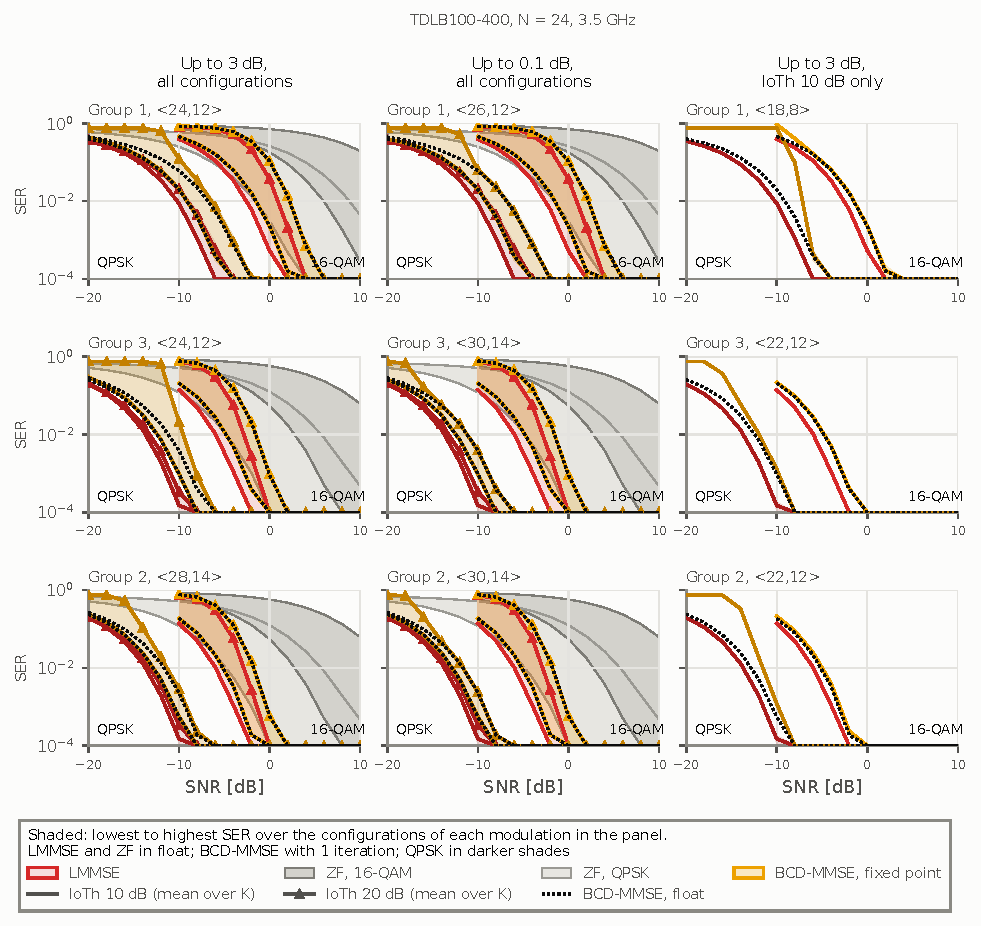
\includegraphics[width=\textwidth]{Images/RESULTADOS/curvas_ser/curvas_ser_grupos_range_B100.pdf}
\vspace{4pt}
\legend{\textcolor{red}{Fonte: a autora.}}
\end{figure}

\begin{figure}[!ht]
\caption{\textcolor{red}{Curvas de SER dos três grupos na TDLA30-5 e na TDLA30-10, nos formatos escolhidos.}}
\label{fig:curvas-range-a30}
\vspace{4pt} % a classe zera o espaço entre a caption e a figura
\centering
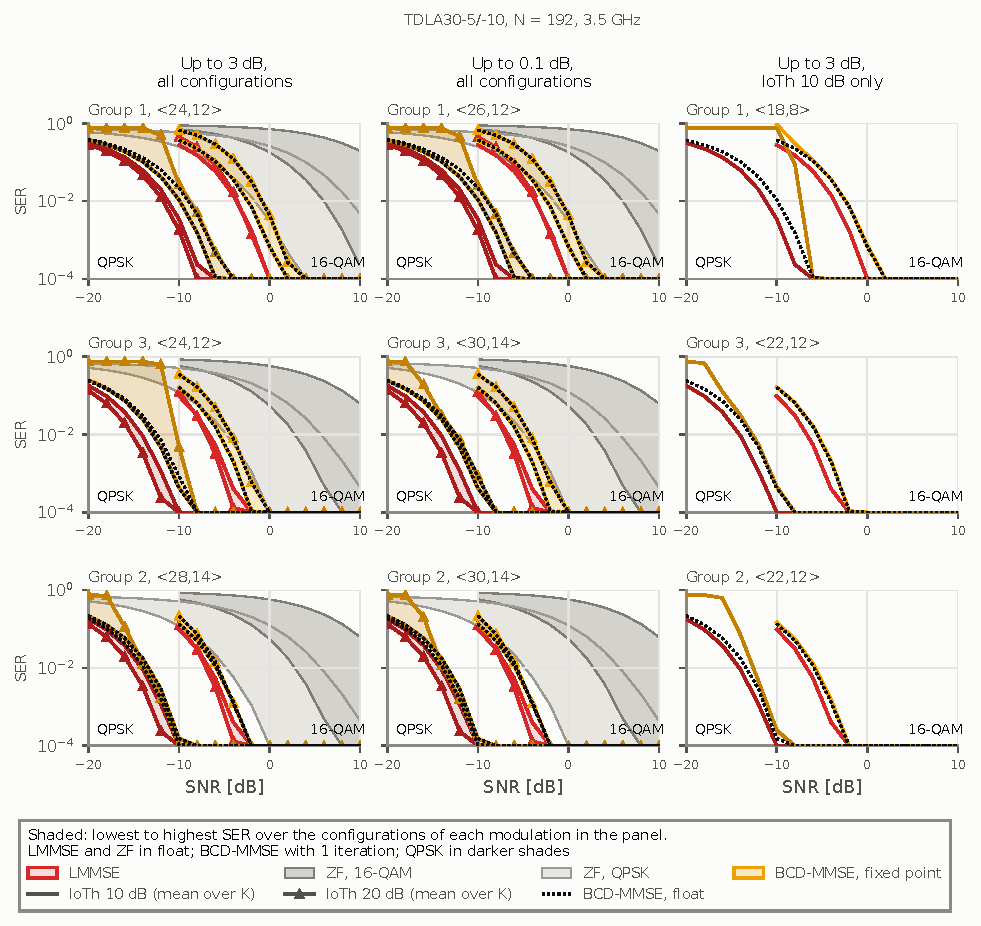
\includegraphics[width=\textwidth]{Images/RESULTADOS/curvas_ser/curvas_ser_grupos_range_A30-5.pdf}
\vspace{4pt}
\legend{\textcolor{red}{Fonte: a autora.}}
\end{figure}

\chapter{\textcolor{red}{SNR increase per configuration}}\label{ap:perfis-configuracao}
% =====================================================================
% APÊNDICE D -- aumento de SNR por configuração, em cada perfil de mobilidade.
% 2026-11-13: texto e figura vieram da seção Mobility profiles (RESULTADOS/formatos.tex);
%   lá ficou só a figura por formato (perfis_mobilidade_formatos). Dados:
%   software/testes/.../figuras/perfis/tcc_perfis_mobilidade_3col_data.csv (figuras_perfis.py).
% =====================================================================

Figure~\ref{fig:perfis-mobilidade} breaks down the largest SNR increase by mobility profile (Section~\ref{subsec:setup_condicoes}). Each point represents the largest increase among the test conditions of a profile. Each row corresponds to a group, and the columns follow the structure of Table~\ref{tab:formatos-escolhidos}: the first two columns include all configurations, the first with the 3~dB format and the second with the 0.1~dB format, while the third column includes only the 10~dB IoTh configurations, with the 3~dB format selected specifically for that subset. When the difference between them exceeds 0.1~dB, the high-mobility profile shows the larger SNR increase (filled point to the right of the unfilled one). The largest observed difference is 0.58~dB, in configuration 2D with $\langle 22,12\rangle$: 0.80~dB for low mobility versus 1.39~dB for high mobility.
% ANTIGO: In all the plots, both mobility profiles meet the criterion of the column. [...] Consequently, the choice of format does not change with the mobility profile.

\begin{figure}[!htb]
\caption{\textcolor{red}{Largest SNR increase, in dB, of each configuration in each mobility profile, in the three groups, with the selected formats.}}
\label{fig:perfis-mobilidade}
\vspace{4pt} % a classe zera o espaço entre a caption e a figura
\centering
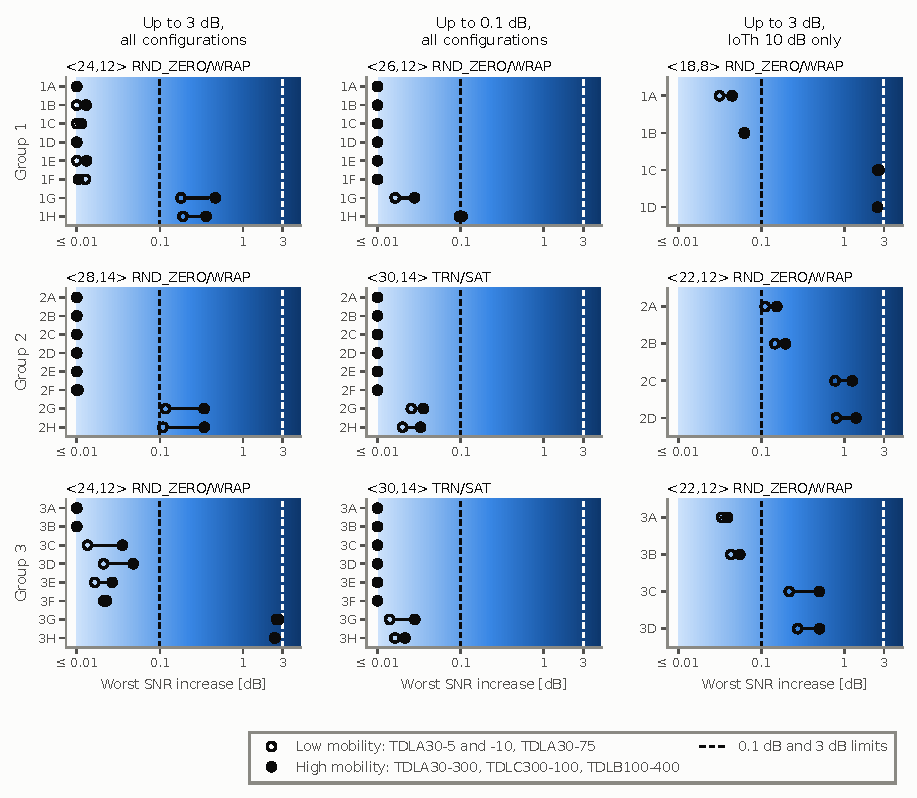
\includegraphics[width=\textwidth]{Images/RESULTADOS/perfis_mobilidade_3col.pdf}
\vspace{4pt}
\legend{\textcolor{red}{Source: the author.}}
\end{figure}


\end{document}
